\documentclass[10pt,twoside]{article}

\usepackage{iftex}

\ifPDFTeX
\usepackage[utf8]{inputenc}
\usepackage[T5]{fontenc}
\usepackage[english]{babel}
\usepackage{mathptmx}
\usepackage[scaled=0.92]{helvet}
\newcommand{\arialfont}{\fontfamily{phv}\selectfont}
\else
\usepackage[english]{babel}
\usepackage{fontspec}
\defaultfontfeatures{Ligatures=TeX}

\IfFontExistsTF{Times New Roman}
{\setmainfont{Times New Roman}}
{\setmainfont{TeX Gyre Termes}}

\IfFontExistsTF{Arial}
{\setsansfont{Arial}\newfontfamily\arialfont{Arial}}
{\setsansfont{TeX Gyre Heros}\newfontfamily\arialfont{TeX Gyre Heros}}
\fi

% ------------------ Page layout based on the FAIR template ------------------
\usepackage[
paperwidth=20.5cm,
paperheight=29.5cm,
top=2.2cm,
bottom=1.8cm,
left=1.8cm,
right=1.8cm,
headheight=13pt,
headsep=0.4cm,
footskip=0.8cm
]{geometry}

% ------------------ Packages ------------------
\usepackage{amsmath,amssymb}
\usepackage{graphicx}
\usepackage{array}
\usepackage{longtable}
\usepackage{caption}
\usepackage{subcaption}
\usepackage{float}
\usepackage{enumitem}
\usepackage{fancyhdr}
\usepackage{titlesec}
\usepackage{indentfirst}
\usepackage{url}
\IfFileExists{cite.sty}{\usepackage{cite}}{}

\newcommand{\fairsmallfont}{\fontsize{9pt}{11pt}\selectfont}
\newcommand{\fairbodyfont}{\fontsize{10pt}{12pt}\selectfont}

\newlength{\fairfigurewidth}
\setlength{\fairfigurewidth}{12cm}

\newcommand{\xairesultcell}[3][\linewidth]{%
  \begin{minipage}[c]{\linewidth}
    \centering
    {\fairsmallfont #2\par}
    \includegraphics[width=#1]{#3}
  \end{minipage}%
}

\newcommand{\xairesultfigure}[4][15cm]{%
\begin{figure}[H]
\centering
\includegraphics[width=#1,height=7.5cm]{#4}
\caption{#2}
\label{fig:#3}
\end{figure}%
}

\newcommand{\modelcurvecell}[2]{%
  \begin{minipage}[c]{\linewidth}
    \centering
    \vspace{2pt}%
    \textbf{#1}\par
    \vspace{1pt}%
    \includegraphics[width=0.85\linewidth]{#2}
    \vspace{1pt}%
  \end{minipage}%
}

% ------------------ Paragraph style ------------------
\setlength{\parindent}{1cm}
\setlength{\parskip}{6pt}
\emergencystretch=2em
\raggedbottom

% ------------------ Paper metadata ------------------
\newcommand{\fairsuperscript}[1]{%
  \raisebox{0.8ex}{\fontsize{8pt}{8pt}\selectfont #1}%
}
\newcommand{\PaperTitle}{CORPORATE CREDIT RATING BASED ON MACHINE LEARNING MODELS}
\newcommand{\PaperShortTitle}{CORPORATE CREDIT RATING BASED ON MACHINE LEARNING MODELS}
\newcommand{\PaperAuthors}{Le Nguyen Thanh Tai\fairsuperscript{1}}
\newcommand{\PaperShortAuthors}{Le Nguyen Thanh Tai}
\newcommand{\PaperAffiliations}{%
\fairsuperscript{1}Faculty of Information Technology, Vinh Long University of Technology Education
}
\newcommand{\PaperEmail}{22022001@st.vlute.edu.vn}
\newcommand{\FairConference}{}

% ------------------ Header/Footer ------------------
\pagestyle{fancy}
\fancyhf{}

% Even pages: page number on the left, paper title on the right.
% Odd pages: author on the left, page number on the right.
\fancyhead[LE,RO]{\fairsmallfont\thepage}
\fancyhead[RE]{\fairsmallfont\PaperShortTitle}
\fancyhead[LO]{\fairsmallfont\PaperShortAuthors}

% The template uses a thin rule below the header on subsequent pages.
\renewcommand{\headrulewidth}{0.4pt}
\renewcommand{\footrulewidth}{0pt}

\fancypagestyle{firstpage}{%
\fancyhf{}%
\fancyhead[C]{\fairsmallfont\FairConference}%
\renewcommand{\headrulewidth}{0.4pt}
}

% ------------------ Title block ------------------
\newcommand{\makefairtitle}{%
\thispagestyle{firstpage}%
\begin{center}
{\arialfont\bfseries\fontsize{14pt}{16pt}\selectfont\MakeUppercase{\PaperTitle}\par}
\vspace{3pt}
{\bfseries\fontsize{12pt}{14pt}\selectfont\PaperAuthors\par}
\vspace{3pt}
{\fairsmallfont\PaperAffiliations\par}
\vspace{3pt}
{\itshape\fairsmallfont\PaperEmail\par}
\end{center}
\vspace{6pt}%
}

% ------------------ Abstract / Keywords ------------------
\newcommand{\FairDash}{\unskip\textemdash\space}

\newenvironment{fairabstract}{%
\begingroup
\fairsmallfont
\itshape
\setlength{\parindent}{1cm}%
\setlength{\parskip}{6pt}%
}{%
\par\endgroup
}

\newcommand{\fairabstracttext}[1]{%
\begin{fairabstract}
\textbf{ABSTRACT}\FairDash #1
\end{fairabstract}
}

\newcommand{\fairkeywords}[1]{%
\begin{fairabstract}
\textbf{Keywords}\FairDash #1
\end{fairabstract}
}

% ------------------ Section numbering ------------------
\setcounter{secnumdepth}{4}

\renewcommand{\thesection}{\Roman{section}}
\renewcommand{\thesubsection}{\Alph{subsection}}
\renewcommand{\thesubsubsection}{\arabic{subsubsection}}
\renewcommand{\theparagraph}{\alph{paragraph}}

\titleformat{\section}
{\centering\fairsmallfont\bfseries}
{\thesection.}{0.5em}{}

\titleformat{\subsection}
{\fairsmallfont\bfseries\itshape}
{\thesubsection.}{0.5em}{}

\titleformat{\subsubsection}
{\fairsmallfont\bfseries\itshape}
{\thesubsubsection.}{0.5em}{}

\titleformat{\paragraph}[block]
{\normalsize}
{\theparagraph.}{0.5em}{}

\titlespacing*{\section}{0pt}{6pt}{6pt}
\titlespacing*{\subsection}{0pt}{6pt}{3pt}
\titlespacing*{\subsubsection}{0pt}{6pt}{3pt}
\titlespacing*{\paragraph}{0pt}{6pt}{3pt}

% ------------------ Figure/Table captions ------------------
\renewcommand{\figurename}{Figure}
\renewcommand{\tablename}{Table}

\captionsetup{
font=normalsize,
labelsep=period,
justification=centering,
singlelinecheck=true,
skip=3pt
}

\setlength{\intextsep}{5pt}
\newcommand{\setupfairsubfigures}{%
  \captionsetup[subfigure]{%
    labelformat=simple,
    labelsep=period,
    font=it,
    justification=centering
  }%
  \renewcommand{\thesubfigure}{\alph{subfigure}}%
}

% ------------------ Lists ------------------
\setlist[itemize]{
leftmargin=1.27cm,
itemsep=0pt,
topsep=0pt,
parsep=0pt
}

% ------------------ Bibliography ------------------
% Keep the REFERENCES title in section style without numbering.
\makeatletter
\renewenvironment{thebibliography}[1]{%
\section*{REFERENCES}%
\fairbodyfont
\hbadness=10000
\setlength{\parskip}{0pt}%
\list{[\arabic{enumiv}]}{%
\settowidth\labelwidth{[#1]}%
\leftmargin\labelwidth
\advance\leftmargin\labelsep
\usecounter{enumiv}%
\let\p@enumiv\@empty
\renewcommand{\theenumiv}{\arabic{enumiv}}%
}%
\sloppy
\clubpenalty4000
\widowpenalty4000
}{%
\endlist
}
\makeatother

\urlstyle{same}

% =========================================================
% DOCUMENT
% =========================================================
\begin{document}

\makefairtitle

\fairabstracttext{%
Corporate credit rating is an important task for assessing financial health, debt-service capacity, and early default risk.
This study develops a credit-rating classification system based on financial data from 1,623 firms with 8,680 observations over the 2005--2016 period. Each observation is represented by 12 financial ratios covering liquidity, leverage, profitability, operating efficiency, and cash flow. The original credit ratings are consolidated into three major groups: Distressed, High Yield, and Investment Grade. The study implements and compares LightGBM, XGBoost, LSTM, TCN, PatchTST, Transformer-LSTM, and GraphSAGE models. In addition to individual models, Fuzzy Ensemble and Dynamic Model Fusion scenarios are constructed to exploit complementary strengths across different architectures. In particular, the DMF-TG scenario combines Transformer-LSTM and GraphSAGE and uses Dynamic Classifier Selection to select the more reliable model for each test sample. Experimental results show that DMF-TG achieves the best performance, with Accuracy of 92.98\%, Precision of 92.67\%, Recall of 92.98\%, and F1-score of 92.60\%. Beyond predictive performance, the study integrates GradientSHAP and LIME to analyze the influence of financial indicators on classification decisions. The results indicate that dynamic model fusion can improve corporate credit-rating performance while increasing transparency and practical applicability in corporate risk assessment.
}

\fairkeywords{%
Corporate credit rating, Machine learning, Deep learning, Ensemble learning, Explainable artificial intelligence.
}

\section{INTRODUCTION}

\subsection{Problem introduction}
As the global economy and financial system continue to be affected by interest-rate volatility, corporate default risk has become a major challenge for capital markets. According to S\&P Global Ratings, 117 defaults were recorded worldwide in 2025; although the number of defaults tended to decline, the total value of distressed debt still exceeded USD 140 billion \cite{noauthor_default_nodate}. In particular, repeat defaults and distressed debt exchanges accounted for nearly 60\% of all default cases, indicating that the financial structures of many firms still contain substantial risk. In Asia, local-currency bond markets continue to expand, creating stronger requirements for information transparency and credit-quality assessment. According to the Asian Development Bank's Asia Bond Monitor, the size of emerging East Asia's bond market reached approximately USD 29.5 trillion by the end of 2025 \cite{bank_asia_2025}. This development increases the demand for objective risk-assessment tools that help investors identify credit quality and price risk premia appropriately. In Vietnam, the corporate bond market is entering a phase of recovery and restructuring after several periods of volatility. According to VIS Rating, the corporate bond market reached approximately VND 1.42 quadrillion by the end of 2025, equivalent to nearly 11\% of GDP, while new issuance increased by 32\% to more than VND 624 trillion \cite{noauthor_vis_nodate}. However, information asymmetry remains a major barrier for investors. Without independent and transparent assessment tools, determining firms' risk levels becomes difficult, reducing confidence and constraining capital flows in the market. Against this background, corporate credit rating plays an important role in supporting the assessment of financial health, debt-service capacity, and default risk. Traditional methods often rely heavily on expert judgment or simple statistical models, whereas real-world financial data are nonlinear, time-varying, and affected by multiple market factors. Therefore, applying machine-learning and deep-learning models to corporate credit rating is necessary to improve predictive capacity and support financial decision-making. In this study, a corporate credit-rating system is developed using machine-learning, deep-learning, and graph-based models to classify firms into three risk groups: Investment Grade (IG), High Yield (HY), and Distressed. In addition to optimizing predictive performance, the study integrates Explainable AI (XAI) techniques to explain the influence of each financial indicator on rating outcomes. This approach not only improves model accuracy but also enhances the transparency, reliability, and practical applicability of the system in corporate credit-risk assessment.

\subsection{Related studies}
Truong Thi Thuy Duong and Le Hai Trung \cite{thuy_ung_2023} evaluated six algorithms on 300 Vietnamese firms over the 2017--2019 period; XGBoost achieved an Accuracy of 87.73\%, outperforming Random Forest at 83.49\%. On a larger dataset, Andersson \cite{andersson_machine_2023} reported that Gradient Boosting achieved an Accuracy of approximately 90\% when predicting ratings issued by Standard \& Poor's, Moody's, and Fitch. Deep-learning architectures extend the ability to exploit temporal dependencies and multimodal information. Kofune et al. \cite{kofune_enhancing_2026} proposed Transformer-LSTM and achieved an Accuracy of 89.96\%. Chen and Long \cite{chen_novel_2020} used Self-Attention in the SMAGRU model, obtaining an Accuracy of 93.33\%. Morthens \cite{morthens_1989-_credit_2024} combined sequential and graph models to exploit temporal financial data and inter-firm relationships; GRU and GRU-GCNGRU achieved 75.25\% and 74.44\%, respectively. Fang et al. \cite{fang_design_2025} combined feature selection, data augmentation, and CNN-BiLSTM-AM on financial text data, achieving an Accuracy of 88\%. For graph-based approaches, Feng et al. \cite{feng_every_2020} proposed CCR-GNN for corporate credit rating and reported an Accuracy of 95\% on data from listed Chinese firms. A subsequent study developed HHGNN to exploit hierarchical structure, heterogeneity, and unlabeled data in corporate networks, achieving an Accuracy of 97.557\% \cite{feng_corporate_2024}. Liu and Kok \cite{liu_prediction_2025} used a Heterogeneous Topological Graph Neural Network for bank credit-rating prediction and achieved an Accuracy of 70.57\%. These results show that the effectiveness of each architecture depends substantially on the data source and evaluation protocol. The present study therefore evaluates tree-based, sequential, and graph-based models under a unified dataset while also examining dynamic fusion mechanisms and prediction explainability. Darwish evaluated six machine-learning algorithms (RF, XGBoost, Logistic Regression, SVM OVO, SVM OVA, and MLP) for corporate credit-rating classification and proposed Random-Forest-based feature selection to improve performance; XGBoost was the best model, achieving 72.03\%, and feature selection improved both Accuracy and computational efficiency \cite{darwish_optimization_2025}. Chowdhury et al. \cite{chowdhury_environmental_2023} studied ESG rating prediction using six machine-learning algorithms on data from 6,166 firms across 73 countries during 2005--2019. The results showed that the Random Forest Classifier achieved the best performance, with an Accuracy of 78.50\%. Variable-importance analysis indicated that lagged ESG scores, firm size, and the debt-to-equity ratio were the most influential factors. Das et al. \cite{das_credit_2023} proposed a method combining tabular financial data with CorpNet, a corporate network constructed from SEC filings. Their study used GNNs together with ensemble machine-learning models in AutoGluon to jointly exploit financial features and inter-firm relationships. The results showed that the proposed method achieved an Accuracy of 86.7\%, demonstrating the effectiveness of incorporating graph information into credit-rating prediction. Yang et al. \cite{yang_deep_2023} proposed the HDNN model for corporate credit-risk prediction on high-dimensional data, combining financial data, supply-chain information, and network data from Compustat and Bloomberg. The study improved DNNs by combining L1 and L2 constraints for feature selection and overfitting control. Experimental results showed that HDNN achieved an Accuracy of 80.12\%.

\section{RELATED WORK}

\subsection{Characteristics of corporate credit rating}

Corporate credit rating assesses a firm's financial credibility and ability to meet debt obligations over a defined period \cite{phu_nghi_nodate}. Rating outcomes support banks, investors, and regulators in credit granting, bond investment, and risk monitoring \cite{hai_mo_2023}. Firms with strong profitability, stable cash flow, and low leverage generally belong to better credit groups, whereas firms with weak cash flow, high debt, or insolvency risk belong to higher-risk groups \cite{thuy_ung_2023}. This study divides ratings into three groups: Investment Grade (IG), High Yield (HY), and Distressed. IG denotes low risk; HY indicates higher risk; and Distressed represents weak financial conditions and high default risk \cite{hung_xep_2023}. The relationships between liquidity, leverage, profitability, and cash-flow indicators and credit risk are often nonlinear and time-varying \cite{hai_mo_2023}. Therefore, this study combines machine learning, deep learning, and explainable artificial intelligence (Explainable AI, XAI) to evaluate classification performance and support interpretation of the roles of financial indicators \cite{gramegna_shap_2021}.
\subsection{Machine-learning models used for training}

\subsubsection{LightGBM model (Light Gradient Boosting Machine)}
LightGBM (Light Gradient Boosting Machine) is an ensemble-learning algorithm in the gradient-boosted decision tree (GBDT) family \cite{ke_lightgbm_2017}. The algorithm uses leaf-wise tree growth and sampling and feature-bundling techniques to reduce computational and memory costs on high-dimensional data.
\subsubsection{XGBoost model (eXtreme Gradient Boosting)}
XGBoost (eXtreme Gradient Boosting) is a scalable implementation of GBDT that combines a regularized objective function with computational optimization techniques \cite{chen_xgboost_2016}. This mechanism helps control model complexity and efficiently handles tabular data.
\subsubsection{Temporal Convolutional Network (TCN)}
Temporal Convolutional Network (TCN) uses causal convolutions and dilated convolutions to process sequential data \cite{bai_empirical_2018}. Compared with recurrent architectures, TCN enables parallel computation and expands the receptive field without violating temporal order.
\subsubsection{Long Short-Term Memory network (LSTM)}
Long Short-Term Memory (LSTM) is a variant of recurrent neural networks that uses memory states and gating mechanisms to reduce the effects of vanishing gradients \cite{hochreiter_long_1997}. As a result, LSTM can learn long-term dependencies in sequential data.
\subsubsection{PatchTST model (Patch Time Series Transformer)}
PatchTST divides time series into subsequences (patches) and uses a Transformer to learn representations across patches \cite{nie_time_2023}. This representation reduces input sequence length and supports the model in capturing both local structure and long-term dependencies.
\subsubsection{Hybrid T-LSTM model (Transformer-Long Short-Term Memory)}
The hybrid T-LSTM (Transformer-Long Short-Term Memory) model \cite{kofune_enhancing_2026} combines Transformer and LSTM components to exploit financial time-series data effectively. In corporate credit rating, financial data not only reflect the state at a single point in time but also express firm-level trends over consecutive periods. Therefore, T-LSTM is used to learn both long-range relationships and sequential dependencies in financial-ratio sequences.
\subsubsection{GraphSAGE graph neural network (Graph Sample and Aggregate)}
GraphSAGE is an inductive node-representation learning framework in which each node representation is formed by aggregating features from the node itself and its neighbors \cite{hamilton_inductive_2018}. Unlike methods that learn a fixed vector for each node, GraphSAGE can generate representations for nodes that were not observed during training.
\subsubsection{Model evaluation metrics} 
\paragraph{Accuracy} 
Accuracy \cite{grandini_metrics_2020} is the ratio of correctly predicted samples to the total number of samples in the dataset. It is a simple and intuitive metric commonly used in classification tasks to evaluate overall model performance. Accuracy is computed as follows: 
\begin{equation} Accuracy = \frac{TP + TN}{TP + TN + FP + FN} 
\end{equation} where: 
\begin{itemize} 
\item $TP$ (True Positive): the number of positive samples correctly predicted. 
\item $TN$ (True Negative): the number of negative samples correctly predicted. 
\item $FP$ (False Positive): the number of negative samples incorrectly predicted as positive. 
\item $FN$ (False Negative): the number of positive samples incorrectly predicted as negative. 
\end{itemize}
\paragraph{Precision} 
Precision \cite{grandini_metrics_2020} measures the proportion of correct positive predictions among all positive predictions. This is especially important in applications where false-positive predictions may have serious consequences.
\begin{equation} 
\mathrm{Precision}=\frac{TP}{TP+FP}
\end{equation}
\paragraph{Recall} 
Recall \cite{grandini_metrics_2020} measures the proportion of correctly predicted positive samples among all actual positive samples. Recall is important in situations where all positive cases need to be detected, even if doing so produces some false positives.
\begin{equation} 
\mathrm{Recall}=\frac{TP}{TP+FN}
\end{equation}
\paragraph{F1-score} 
F1-score \cite{grandini_metrics_2020} is the harmonic mean of Precision and Recall. This metric balances the correctness of positive predictions and the ability to detect positive samples.
\begin{equation} 
F1=2\times\frac{\mathrm{Precision}\times\mathrm{Recall}}{\mathrm{Precision}+\mathrm{Recall}}
\end{equation}
\paragraph{AUC-ROC} 
The ROC Curve represents the relationship between the True Positive Rate (Recall) and the False Positive Rate. AUC is the area under the ROC curve and expresses the model's ability to discriminate between classes \cite{fawcett_introduction_2006}. A model with AUC close to 1 is considered strong, whereas AUC close to 0.5 indicates performance similar to random guessing.
\begin{equation} 
\mathrm{TPR}=\frac{TP}{TP+FN}\quad;\quad \mathrm{FPR}=\frac{FP}{FP+TN}
\end{equation}


\subsection{Ensemble-learning methods}

\subsubsection{Fuzzy Choquet Integral}
The Fuzzy Choquet Integral is an ensemble-learning method based on fuzzy measures and is used to aggregate the outputs of multiple component models. Unlike conventional voting or averaging, this method considers not only the individual importance of each model but also the interaction relationships among models in the ensemble \cite{zadeh_fuzzy_1965, choquet_theory_1954}.

Assume that there are $M$ base models $h_1,h_2,\ldots,h_M$. For a data sample $x$, the predicted probability of the $i$-th model for class $c$ is denoted by $p_i^{(c)}$. The set of predicted probabilities for class $c$ is represented as:

\begin{equation}
    f_c = \left\{p_1^{(c)}, p_2^{(c)}, \ldots, p_M^{(c)}\right\}.
\end{equation}

The Choquet integral uses a fuzzy measure $\mu$ satisfying $\mu(\emptyset)=0$, $\mu(H)=1$, and monotonicity $A \subseteq B \Rightarrow \mu(A) \leq \mu(B)$. The probabilities $p_i^{(c)}$ are sorted in ascending order according to a permutation $\sigma$:

\begin{equation}
    p_{\sigma(1)}^{(c)} \leq p_{\sigma(2)}^{(c)} \leq \cdots \leq p_{\sigma(M)}^{(c)}.
\end{equation}

The aggregated score for class $c$ is then computed as:

\begin{equation}
    C_{\mu}(f_c) =
    \sum_{i=1}^{M}
    \left[p_{\sigma(i)}^{(c)} - p_{\sigma(i-1)}^{(c)}\right]
    \mu(A_{\sigma(i)}),
\end{equation}

where $p_{\sigma(0)}^{(c)}=0$ and $A_{\sigma(i)}=\{h_{\sigma(i)},h_{\sigma(i+1)},\ldots,h_{\sigma(M)}\}$. After Choquet scores are computed for all classes, the final predicted label is determined by the class with the largest aggregated score:

\begin{equation}
    \hat{y} = \arg\max_c C_{\mu}(f_c).
\end{equation}

In corporate credit rating, the Fuzzy Choquet Integral flexibly combines predicted probabilities from multiple models, especially when the models are complementary or mutually dependent.

\subsubsection{Gompertz Fuzzy Ranking}

Gompertz Fuzzy Ranking is an ensemble-learning method based on fuzzy ranks and is adapted from the study \textit{Fuzzy rank-based fusion of CNN models using Gompertz function for screening COVID-19 CT-scans} \cite{kundu_fuzzy_2021}. In the original study, the method was used to fuse outputs from multiple CNN models for COVID-19 CT-scan screening. In this study, however, the idea of fuzzy ranking using the Gompertz function is transferred and adapted to the corporate credit-rating problem. Therefore, citation \cite{kundu_fuzzy_2021} is used as a methodological basis for fuzzy rank-based fusion rather than as direct empirical evidence in the credit-rating domain.

Assume that there are $M$ component models and $K$ credit-rating classes. For a data sample $x$, the probability that model $m$ predicts the sample as belonging to class $c$ is denoted by $p_{m,c}$, with $m=1,2,\ldots,M$ and $c=1,2,\ldots,K$. For each class $c$, the predicted probabilities are sorted in ascending order as follows:

\begin{equation}
    p_{\sigma(1),c} \leq p_{\sigma(2),c} \leq \cdots \leq p_{\sigma(M),c},
\end{equation}
where $\sigma$ is the model-index permutation after sorting. Each rank position is normalized to the interval $[0,1]$:

\begin{equation}
    r_i = \frac{i-1}{M-1}, \quad i=1,2,\ldots,M.
\end{equation}

The Gompertz function is used to transform normalized ranks into fuzzy weights:

\begin{equation}
    w_i = \exp\left(-b\exp(-a r_i)\right),
\end{equation}
where $b>0$ and $a>0$ are parameters that control the shape of the Gompertz function. This function increases nonlinearly with rank; therefore, models with higher predicted probabilities receive larger weights, whereas models with lower probabilities are retained but contribute less.

The aggregated score for class $c$ is computed as the weighted average of the sorted probabilities:

\begin{equation}
    S_c = \frac{\sum_{i=1}^{M} w_i p_{\sigma(i),c}}
    {\sum_{i=1}^{M} w_i}.
\end{equation}

After aggregated scores are calculated for all classes, these scores are normalized into the final probability distribution:

\begin{equation}
    \hat{p}_c = \frac{S_c}{\sum_{j=1}^{K} S_j}.
\end{equation}

The final predicted label is determined by the class with the largest aggregated probability:

\begin{equation}
    \hat{y} = \arg\max_c \hat{p}_c.
\end{equation}

In the thesis experiments, the Gompertz-function parameters are optimized on the validation set to better fit the characteristics of financial data. This approach enables the system to exploit both predicted probabilities and relative model confidence, which is particularly suitable for a problem with class boundaries that are not fully clear, such as Distressed, HY, and IG.

\subsubsection{Dynamic Model Fusion}

Dynamic Model Fusion (DMF) is a dynamic model-combination method adapted from the study \textit{Explainable dynamic fusion of GCNN and CNN for precise brain tumor analysis from MRI scans} by Toufiq and Pal \cite{toufiq_explainable_2026}. In the original study, DMF was used to combine GCNN and CNN for brain MRI analysis. In this thesis, the DMF idea is transferred and adapted to corporate credit rating. Therefore, citation \cite{toufiq_explainable_2026} is used as a methodological basis for dynamic fusion and model selection, rather than as direct empirical evidence in the credit-rating domain.

Assume that there are $m$ component classifiers $c_1,c_2,\ldots,c_m$. For a test sample $x_t$, model $c_j$ produces a predicted label $o_j$ and the corresponding confidence probability $p_j(o_j|x_t)$:

\begin{equation}
    o_j = c_j(x_t), \quad j=1,2,\ldots,m.
\end{equation}

If all component models produce the same label, the system directly selects that consensus label as the final output:

\begin{equation}
    \hat{y} = o_1, \quad \text{when } o_1=o_2=\cdots=o_m.
\end{equation}

When models disagree, DCS computes a dynamic selection score for each model based on two components: the model's competence on the validation set and its confidence for the test sample. Let $\delta_j$ denote the competence score of model $c_j$ on the validation set for the class predicted by that model, and let $v_j$ denote the model-priority weight. The dynamic selection score is then defined as:

\begin{equation}
    S_j = \delta_j \cdot v_j + p_j(o_j|x_t),
\end{equation}
where $S_j$ is the dynamic selection score of model $c_j$, $\delta_j$ reflects the model's predictive competence on the validation set, $v_j$ is the priority weight, and $p_j(o_j|x_t)$ is the model's confidence probability for the current test sample. In the main experimental setting, all weights are set equally, i.e., $v_j=1$.

The model with the highest dynamic selection score is selected as the winning model:

\begin{equation}
    w = \arg\max_{j} S_j.
\end{equation}

The final predicted label is determined by the label of the winning model:

\begin{equation}
    \hat{y} = o_w.
\end{equation}

Thus, DMF enables the system to select an appropriate model for each data sample instead of applying a fixed fusion rule. When the models agree, the system uses the common label; when they disagree, DCS selects the more reliable model based on both validation competence and test-sample prediction probability. This approach helps the system adapt better to complex financial data or ambiguous classification boundaries among Distressed, HY, and IG.

\subsection{Explainable artificial intelligence methods}
\subsubsection{GradientSHAP} 
GradientSHAP is a gradient-based explanation method that combines the idea of SHAP with random sampling between the target data and background samples. The method estimates each feature's contribution by computing gradients of the model output with respect to the input at multiple interpolation points between the sample to be explained and baseline samples \cite{lundberg_unified_2017, kokhlikyan_captum_2020}. 
\subsubsection{LIME} 
LIME is a model-agnostic local explanation method proposed by Ribeiro et al. to explain a specific prediction using a simple model in the neighborhood of the sample being analyzed \cite{ribeiro_why_2016}. The main idea of LIME is to generate many perturbed samples around the original observation, pass these samples through the model to obtain predicted probabilities, and then train a locally weighted linear model to approximate the behavior of the original model.

\section{PROPOSED METHOD}

This study proposes a system consisting of two phases: training and testing. The overall workflow is presented in Figure~\ref{fig:proposed_model}.
\begin{figure}[H]
    \centering
    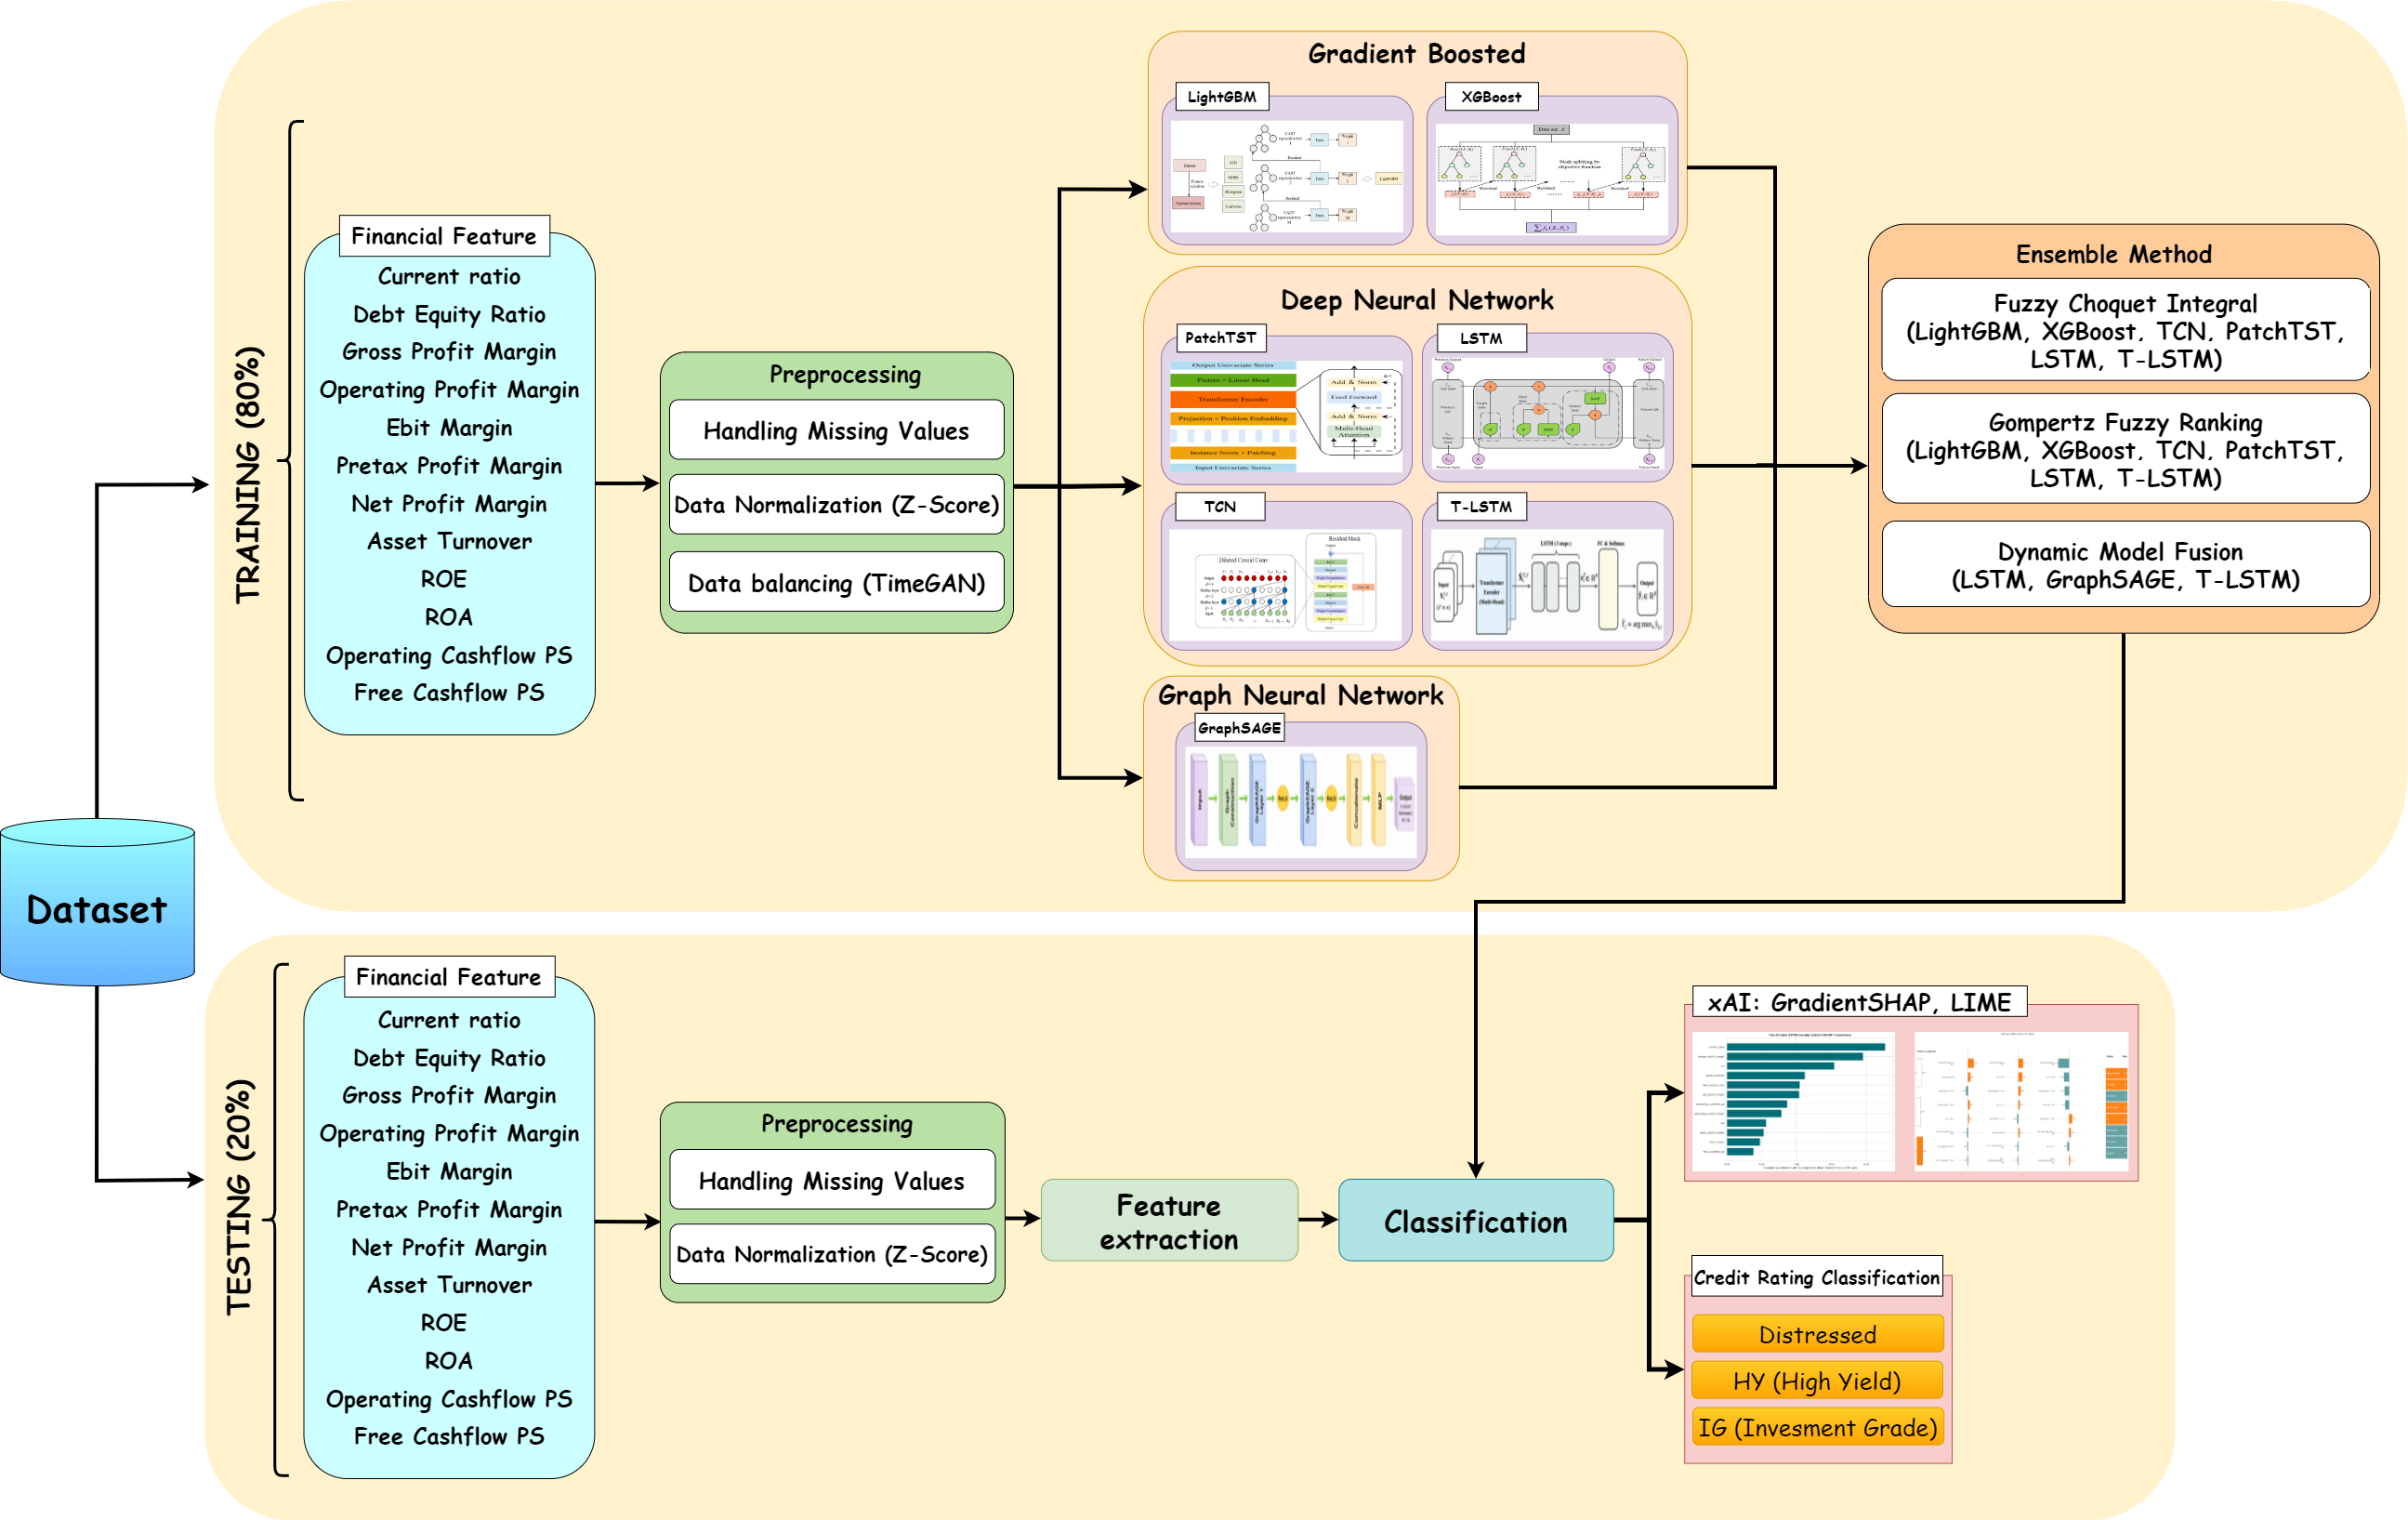
\includegraphics[width=\textwidth]{acc-loss/diagram_pipeline_overview.png}
    \caption{Proposed model}
    \label{fig:proposed_model}
\end{figure}
\subsection{Training phase} 
\subsubsection{Data preprocessing and data preparation} 
Data preprocessing is an important step to ensure that the input data are suitable for the corporate credit-rating problem and that models can learn more stably. In this study, the data are processed from 12 financial indicators reflecting liquidity, leverage, profitability, operating efficiency, and cash flow. First, duplicate records by ticker and rating date are merged, and missing values are imputed using the median of the training set to reduce the influence of outliers and avoid data leakage.

Next, skewed financial features are transformed to reduce skewness, and the data are then standardized using Z-score normalization to place indicators with different scales on a common reference scale. In addition, the original dataset contains 21 distinct credit ratings, including D, C, CC, CCC-, CCC, CCC+, B-, B, B+, BB-, BB, BB+, BBB-, BBB, BBB+, A-, A, A+, AA-, AA, AA+, and AAA. Because the number of samples varies substantially across rating classes, especially with fewer high-risk ratings, this study consolidates the 21 ratings into three major groups: Distressed, High Yield (HY), and Investment Grade (IG). Specifically, the Distressed group includes ratings from C to CCC+, representing firms with very high credit risk or severe financial distress. The High Yield (HY) group includes ratings from B- to BB+, reflecting firms with medium to high risk but not yet in distress. The Investment Grade (IG) group includes ratings from BBB- to AAA, representing firms with good repayment capacity and low credit risk. This grouping reduces data imbalance while aligning with the objective of classifying credit risk into three major levels. Finally, the data are structured into firm-level time series using a sliding-window technique. These sequences are used for time-series deep-learning models such as LSTM, TCN, PatchTST, and T-LSTM. To mitigate class imbalance, especially in the Distressed group, this study uses TimeGAN to generate additional synthetic financial sequences with characteristics similar to the original data. As a result, the training set becomes more balanced, helping models improve generalization and better identify firms with high credit risk.
\subsubsection{Feature extraction and training}
After preprocessing, financial-indicator sequences are fed into models for feature extraction and training. Input data are organized as sliding windows, enabling the models to exploit firm-level changes across consecutive time periods. Feature extraction is performed automatically by deep-learning models such as LSTM, TCN, PatchTST, and T-LSTM. These models learn directly from standardized financial sequences, including indicator values, temporal trends, and relationships among features over time. During training, all models are trained independently on the same dataset and under the same preprocessing pipeline to ensure fairness in comparison. The AdamW algorithm is used to optimize weights, combined with the Cross Entropy loss for the three-class classification problem involving IG, HY, and Distressed. To improve stability and reduce overfitting, Gradient Clipping is applied during backpropagation. At the same time, Loss, Accuracy, and F1-score are monitored on the training and validation sets. Model selection based on F1-score provides a more balanced evaluation across classes, particularly in the context of imbalanced credit-rating data.

\subsection{Testing phase}
After training is complete, the models enter the testing phase to evaluate generalization on unseen data. In this stage, each model is switched to evaluation mode to ensure stable inference without parameter updates. Model outputs are predicted labels belonging to the three credit-rating groups: IG, HY, and Distressed. Testing is conducted for both individual models and fusion scenarios. The individual models include LightGBM, XGBoost, LSTM, TCN, PatchTST, T-LSTM, and GraphSAGE. In addition, this study constructs Fuzzy Ensemble combinations such as TTX, PLL, and TTLPXL, using the Fuzzy Choquet Integral and Gompertz Fuzzy Ranking to combine predicted probabilities from multiple models. Dynamic Model Fusion scenarios, including DMF-LG, DMF-LT, DMF-TG, and DMF-LTG, are also implemented to select the appropriate model for each data sample through Dynamic Classifier Selection. Model performance is evaluated using multiple metrics, including Accuracy, Precision, Recall, F1-score, AUC-ROC, confusion matrix, and inference time. These metrics comprehensively assess overall classification ability and the effectiveness of identifying each credit-rating class. In particular, the confusion matrix is used to analyze prediction errors among the three groups IG, HY, and Distressed. Beyond performance evaluation, the testing phase integrates Explainable AI methods including GradientSHAP and LIME. GradientSHAP is used to determine the influence of each financial indicator on prediction outcomes, whereas LIME supports local explanations for specific firm-level cases. Therefore, testing results demonstrate not only classification effectiveness but also interpretability, increasing the transparency and reliability of the corporate credit-rating system.


\section{EXPERIMENTAL RESULTS}

\subsection{Experimental environment and dataset}

\subsubsection{Experimental environment}
The experiments are conducted on Kaggle Notebooks \cite{noauthor_notebooks_nodate}, using an Intel Xeon 2.00 GHz CPU with 4 vCPUs, 32 GB RAM, and an NVIDIA Tesla P100 GPU with 16 GB VRAM. The models are implemented in Python 3.8+ and PyTorch. Pandas and NumPy are used for data processing, while Matplotlib and Scikit-learn support visualization and evaluation. Kaggle's GPU time limit is considered when selecting batch size and memory configuration.

\subsubsection{Experimental dataset}
The dataset is compiled from two public sources on Kaggle: \textit{Corporate Credit Rating} \cite{noauthor_corporate_credit_rating_nodate} and \textit{Corporate Credit Rating with Financial Ratios} \cite{noauthor_corporate_financial_ratios_nodate}. The two sources are linked by company name, ticker, rating agency, and rating date. After cleaning, merging, and duplicate removal, the data contain 8,680 observations from 1,623 firms over the 2005--2016 period. Each observation includes 12 financial indicators: Current Ratio, Debt-to-Equity Ratio, Gross Profit Margin, Operating Profit Margin, EBIT Margin, Pretax Profit Margin, Net Profit Margin, ROE, ROA, Asset Turnover, Operating Cash Flow per Share, and Free Cash Flow per Share. These indicators represent liquidity, leverage, profitability, operating efficiency, and cash flow. The original 21 credit ratings are grouped into three classes: IG, HY, and Distressed. Each firm has approximately 5.35 ratings on average, so the dataset has both tabular structure and temporal characteristics. To reduce data leakage across firms, the training, validation, and test sets are split independently by ticker. The class distribution after label grouping is shown in Table~\ref{tab:class_distribution}.
\begin{table}[H] 
\centering 
\caption{Detailed class distribution in the original split} 
\label{tab:class_distribution} 
\begin{tabular}{lccc} 
\hline \textbf{Class} & \textbf{Train} & \textbf{Val} & \textbf{Test} \\ \hline Investment Grade (IG) & 3898 & 557 & 1114 \\ High Yield (HY) & 1970 & 281 & 563 \\ Distressed & 208 & 30 & 59 \\ \hline 
\end{tabular} 
\end{table}
\subsection{Experimental scenarios}

Seventeen experimental scenarios are divided into two groups. The first group consists of seven individual, hybrid, and graph-based models: LightGBM, XGBoost, TCN, LSTM, PatchTST, T-LSTM, and GraphSAGE. The second group consists of ensemble-learning scenarios using Fuzzy Choquet Integral (FI), Gompertz Fuzzy Ranking (FR), or Dynamic Model Fusion (DMF). The configuration of each scenario is presented in Table~\ref{tab:experimental_scenarios}.

\begingroup
\centering
\begin{longtable}{c l l >{\raggedright\arraybackslash}p{6.5cm}}
\caption{Experimental scenarios}
\label{tab:experimental_scenarios}\\
\hline 
\textbf{Scenario} & \textbf{Scenario name} & \textbf{Fusion method} & \textbf{Models used} \\ \hline 
1 & LightGBM & -- & LightGBM \\ 
2 & XGBoost & -- & XGBoost \\ 
3 & TCN & -- & Temporal Convolutional Networks (TCN) \\ 
4 & LSTM & -- & Long Short-Term Memory (LSTM) \\ 
5 & PatchTST & -- & Patch Time Series Transformer (PatchTST) \\ 
6 & T-LSTM & -- & Transformer--Long Short-Term Memory (T-LSTM) \\ 
7 & GraphSAGE & -- & GraphSAGE, Multilayer Perceptron (MLP) \\ 
8 & FI-TTX & Fuzzy Choquet Integral & TCN + T-LSTM + XGBoost \\ 
9 & FI-PLL & Fuzzy Choquet Integral & PatchTST + LSTM + LightGBM \\ 
10 & FI-TTLPXL & Fuzzy Choquet Integral & TCN + T-LSTM + LSTM + PatchTST + XGBoost + LightGBM \\ 
11 & FR-TTX & Gompertz Fuzzy Ranking & TCN + T-LSTM + XGBoost \\ 
12 & FR-PLL & Gompertz Fuzzy Ranking & PatchTST + LSTM + LightGBM \\ 
13 & FR-TTLPXL & Gompertz Fuzzy Ranking & TCN + T-LSTM + LSTM + PatchTST + XGBoost + LightGBM \\ 
14 & DMF-LG & Dynamic Model Fusion & LSTM + GraphSAGE \\ 
15 & DMF-LT & Dynamic Model Fusion & LSTM + T-LSTM \\ 
16 & DMF-TG & Dynamic Model Fusion & T-LSTM + GraphSAGE \\
17 & DMF-LTG & Dynamic Model Fusion & LSTM + T-LSTM + GraphSAGE \\ \hline
\end{longtable}
\endgroup

\begin{table}[H] 
\centering 
\caption{Training parameters for the scenarios} 
\label{tab:hyperparameter} 
\begin{tabular}{c c c l c} 
\hline 
\textbf{Scenario} & \textbf{Learning rate} & \textbf{Epochs} & \textbf{Loss function} & \textbf{Classes} \\ 
\hline 
1 & 3e-2 & 100 & Cross Entropy & 3 \\ 
2 & 3e-2 & 100 & Cross Entropy & 3 \\ 
3 & 3e-4 & 100 & Cross Entropy & 3 \\ 
4 & 3e-4 & 100 & Cross Entropy & 3 \\ 
5 & 3e-4 & 100 & Cross Entropy & 3 \\ 
6 & 3e-4 & 100 & Cross Entropy & 3 \\ 
7 & 6e-4 & 100 & Cross Entropy & 3 \\ 
\hline 
\end{tabular} 
\end{table}

Table~\ref{tab:hyperparameter} presents the training parameters configured for each experimental scenario. For LightGBM and XGBoost, a learning rate of $3\times10^{-2}$ is used in the boosting mechanism to control the contribution of each decision tree to the overall model; the number of learning iterations corresponds to the number of boosting rounds. For deep-learning models such as TCN, LSTM, PatchTST, and T-LSTM, a smaller learning rate of $3\times10^{-4}$ is selected to stabilize weight updates and reduce oscillation when processing financial time-series data. GraphSAGE uses the AdamW optimizer with a learning rate of $6\times10^{-4}$ to stabilize node-representation learning on the graph. All scenarios use the Cross Entropy loss function for the multiclass classification problem involving three credit-rating groups: Distressed, HY, and IG.
\subsection{Training results}

\begin{table}[H]
\centering
\caption{Summary of model training results (\%)}
\label{tab:training_results}
\begin{tabular}{c l c c c c}
\hline
\textbf{Scenario} & \textbf{Training network} & \textbf{Train Loss} & \textbf{Val Loss} & \textbf{Train Acc} & \textbf{Val Acc} \\
\hline
1 & LightGBM  & 0.123 & 0.266 & 94.0 & 92.0 \\
2 & XGBoost   & 0.177 & 0.267 & 94.0 & 92.4 \\
3 & TCN       & 0.248 & 0.276 & 92.7 & 92.3 \\
4 & LSTM      & 0.190 & 0.268 & 94.0 & 92.2 \\
5 & PatchTST  & 0.217 & 0.279 & 93.2 & 91.7 \\
6 & T-LSTM    & 0.167 & 0.223 & 94.0 & 92.4 \\
7 & GraphSAGE & 0.343 & 0.399 & 92.1 & 92.2 \\
\hline
\end{tabular}
\end{table}
\subsubsection{Accuracy}
\begin{figure}[H]
    \centering
    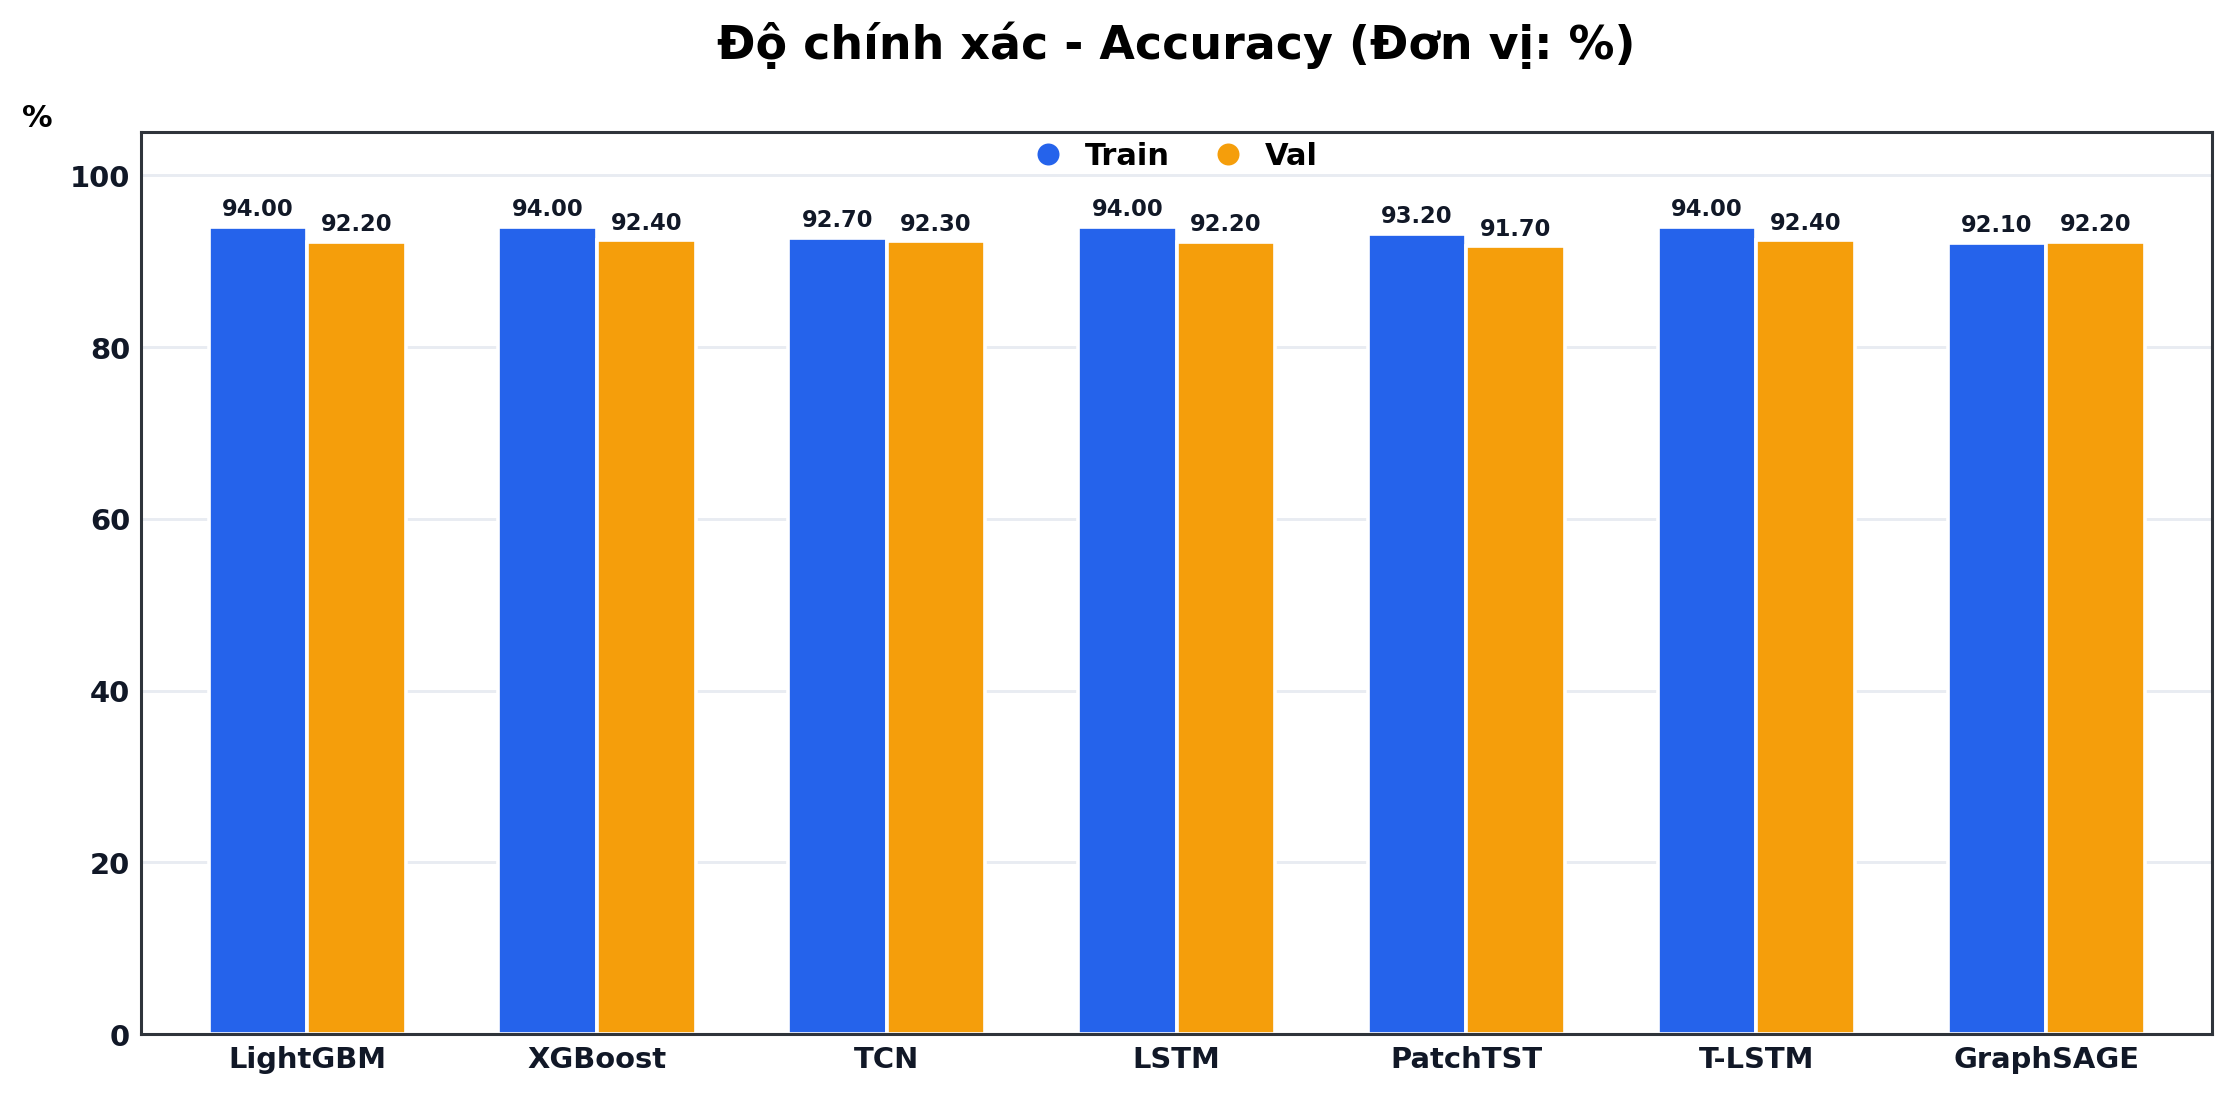
\includegraphics[width=\fairfigurewidth]{acc-loss/curve_accuracy_overall.png}
    \caption{Accuracy chart}
    \label{tab:acc-train}
\end{figure}

Figure~\ref{tab:acc-train} shows that training Accuracy ranges from 92.10\% to 94.00\%, while validation Accuracy ranges from 91.70\% to 92.40\%. XGBoost and T-LSTM jointly achieve the highest validation Accuracy at 92.40\%. TCN and GraphSAGE show gaps between the two sets of 0.40 and 0.10 percentage points, respectively. PatchTST obtains the lowest validation Accuracy at 91.70\%. The 0.70-percentage-point range indicates that validation-set differences among models are relatively small. The detailed accuracy curves during training are presented in Table~\ref{tab:accuracy_models}.

\begingroup
\centering
\renewcommand{\arraystretch}{1.2}
\setlength{\tabcolsep}{0pt}
\begin{longtable}{>{\centering\arraybackslash}p{0.48\textwidth}|
                  >{\centering\arraybackslash}p{0.48\textwidth}}
\caption{Model accuracy}
\label{tab:accuracy_models}\\
\hline
\modelcurvecell{Scenario 1: LightGBM}{acc-loss/curve_accuracy_lightgbm.png} &
\modelcurvecell{Scenario 2: XGBoost}{acc-loss/curve_accuracy_xgboost.png} \\
\hline
\modelcurvecell{Scenario 3: TCN}{acc-loss/curve_accuracy_tcn.png} &
\modelcurvecell{Scenario 4: LSTM}{acc-loss/curve_accuracy_lstm.png} \\
\hline
\modelcurvecell{Scenario 5: PatchTST}{acc-loss/curve_accuracy_patchtst.png} &
\modelcurvecell{Scenario 6: T-LSTM}{acc-loss/curve_accuracy_tlstm.png} \\
\hline
\modelcurvecell{Scenario 7: GraphSAGE}{acc-loss/curve_accuracy_graphsage.png} & \\
\hline
\end{longtable}
\endgroup


\subsubsection{Loss}
\begin{figure}[H]
    \centering
    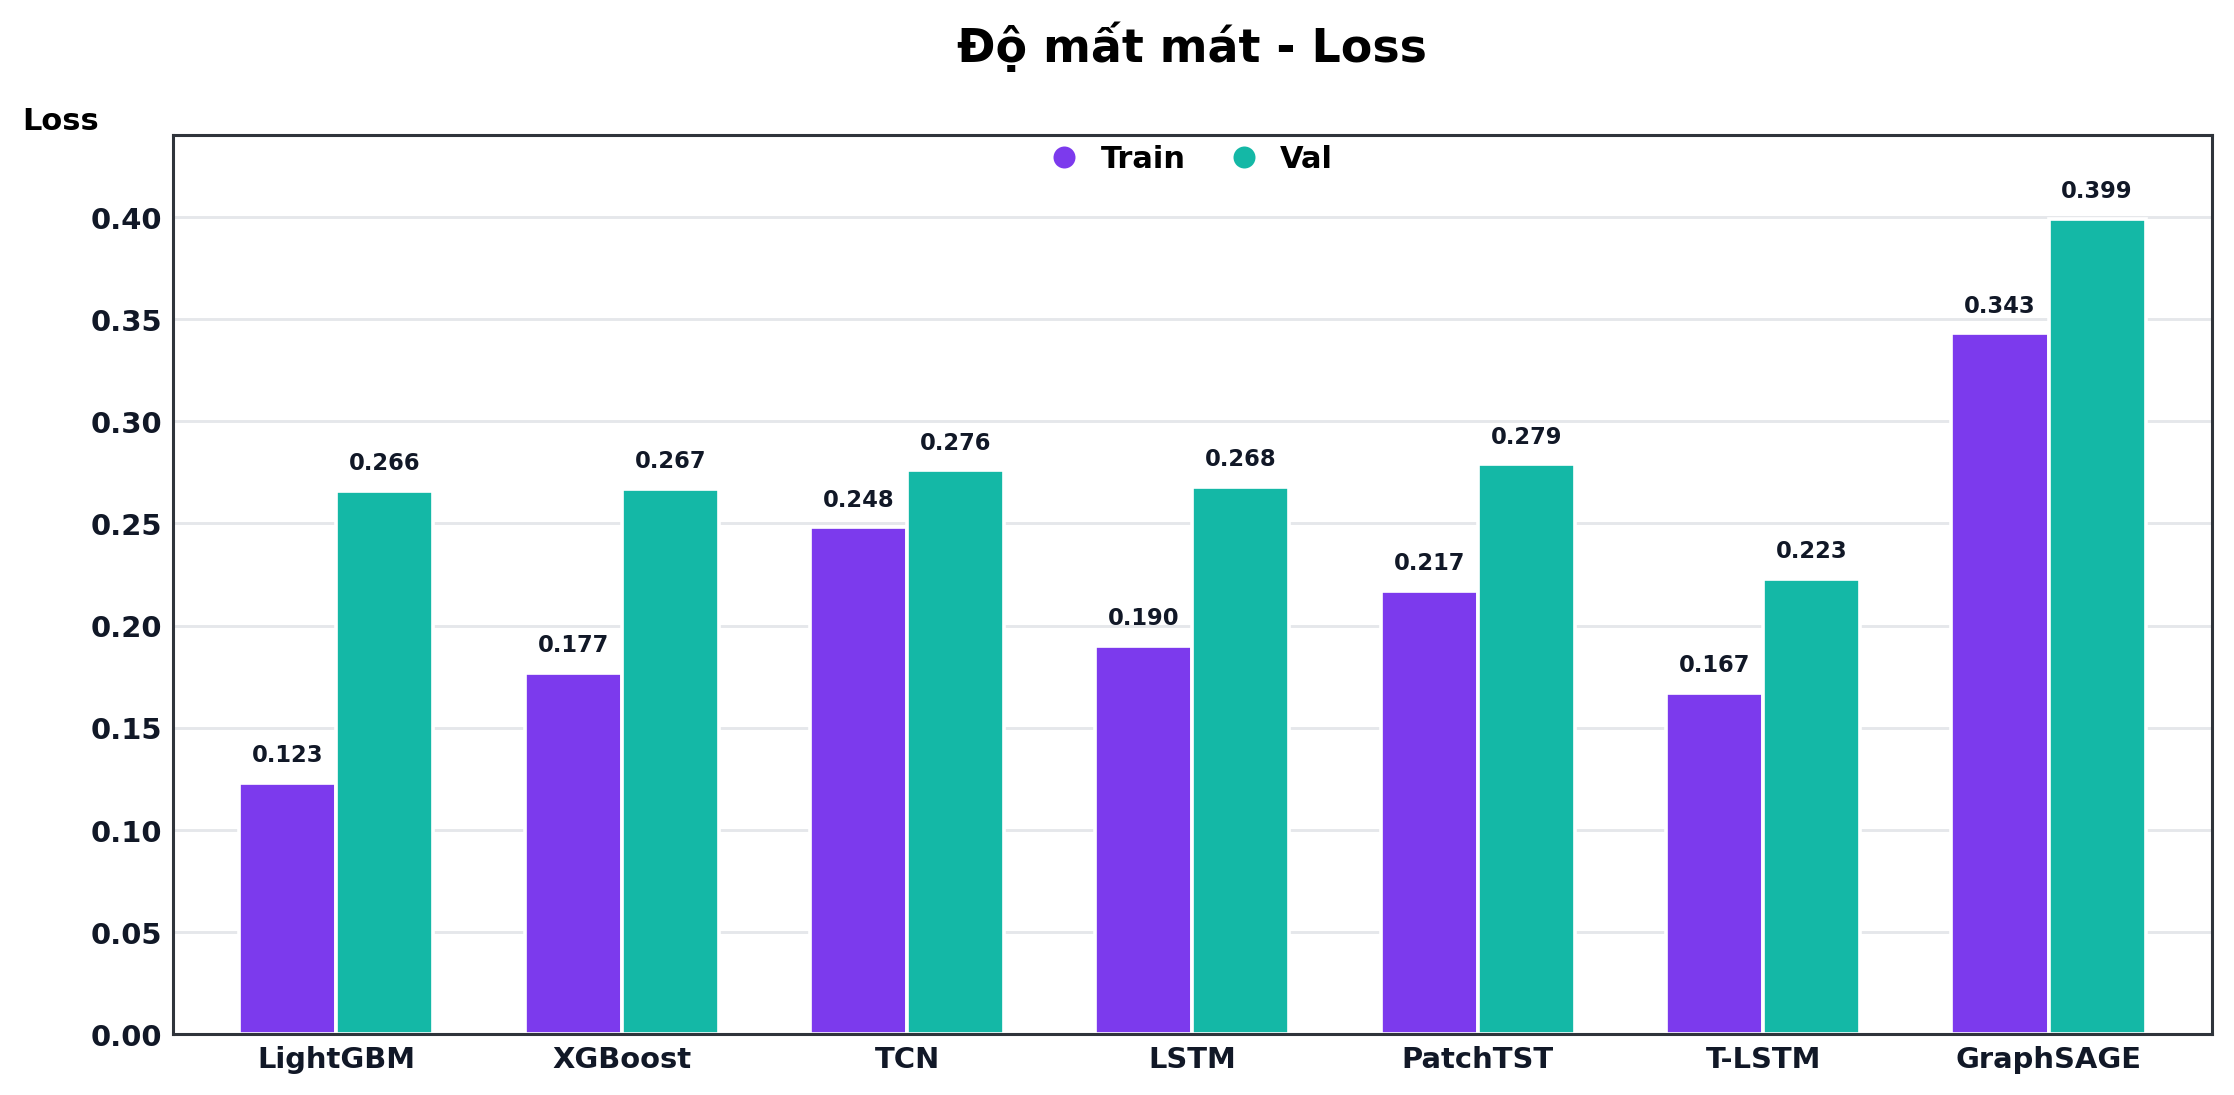
\includegraphics[width=\fairfigurewidth]{acc-loss/curve_loss_overall.png}
    \caption{Loss chart}
\end{figure}

Training loss ranges from 0.123 to 0.343; on the validation set, the values range from 0.223 to 0.399. T-LSTM has the lowest validation loss (0.223), followed by LightGBM (0.266), XGBoost (0.267), and LSTM (0.268). GraphSAGE records the highest values on both the training set (0.343) and the validation set (0.399). These descriptive results indicate that T-LSTM maintains a low validation loss, although they are not sufficient to conclude that the differences among models are statistically significant. The detailed loss curves during training are presented in Table~\ref{tab:loss_models}.

\begingroup
\centering
\renewcommand{\arraystretch}{1.2}
\setlength{\tabcolsep}{0pt}
\begin{longtable}{>{\centering\arraybackslash}p{0.48\textwidth}|
                  >{\centering\arraybackslash}p{0.48\textwidth}}
\caption{Model loss}
\label{tab:loss_models}\\
\hline

\modelcurvecell{Scenario 1: LightGBM}{acc-loss/curve_loss_lightgbm.png} &
\modelcurvecell{Scenario 2: XGBoost}{acc-loss/curve_loss_xgboost.png} \\
\hline

\modelcurvecell{Scenario 3: TCN}{acc-loss/curve_loss_tcn.png} &
\modelcurvecell{Scenario 4: LSTM}{acc-loss/curve_loss_lstm.png} \\
\hline

\modelcurvecell{Scenario 5: PatchTST}{acc-loss/curve_loss_patchtst.png} &
\modelcurvecell{Scenario 6: T-LSTM}{acc-loss/curve_loss_tlstm.png} \\
\hline

\modelcurvecell{Scenario 7: GraphSAGE}{acc-loss/curve_loss_graphsage.png} & \\
\hline
\end{longtable}
\endgroup

\subsubsection{Training time}

\begin{figure}[H]
    \centering
    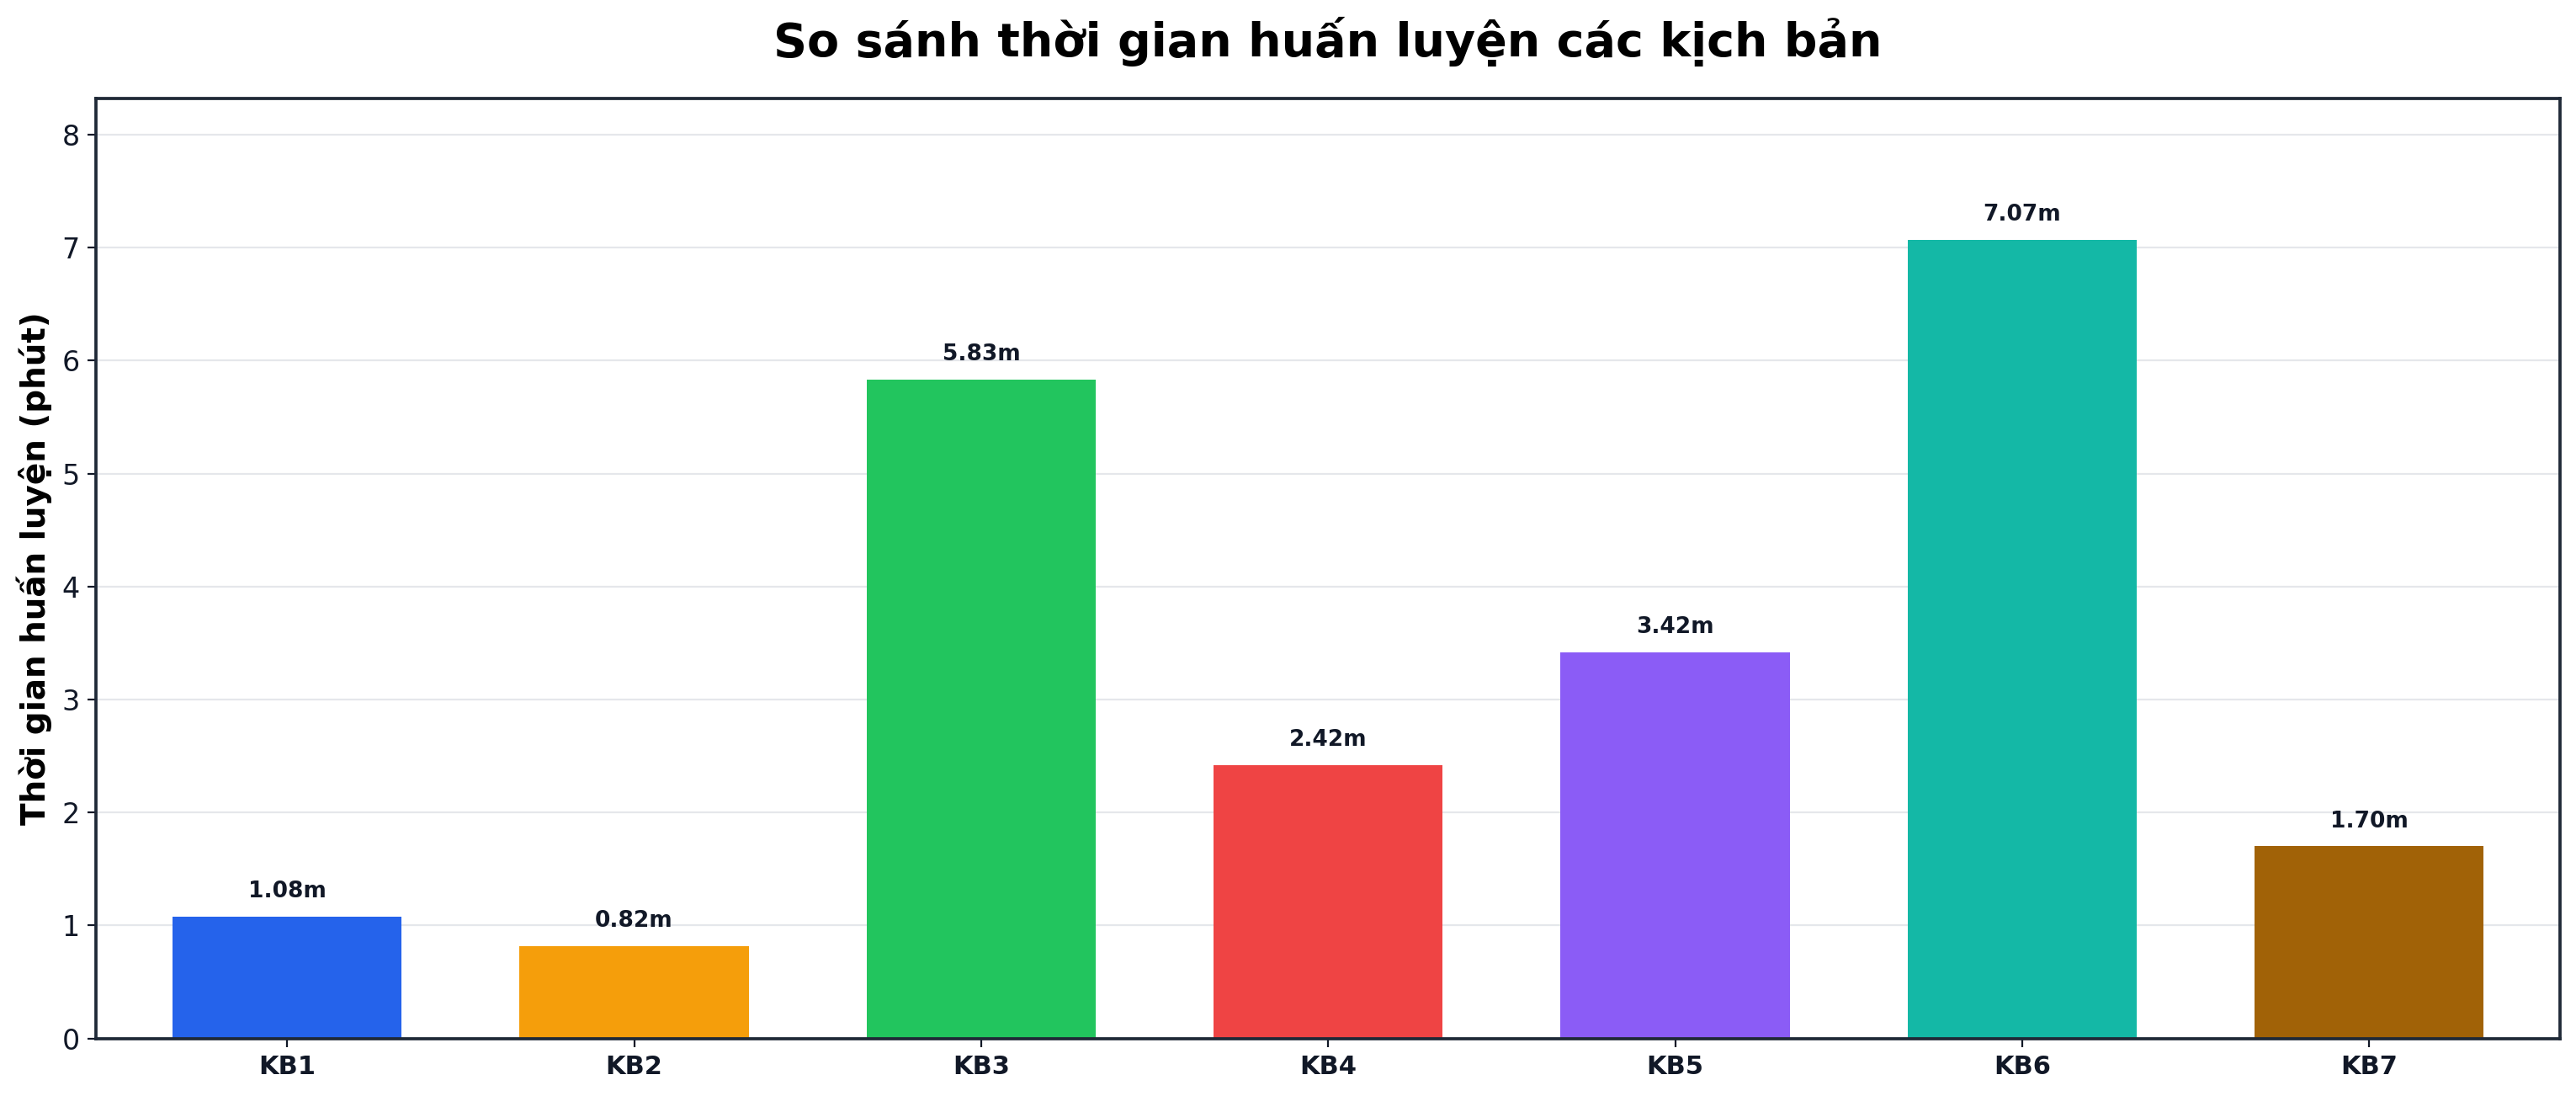
\includegraphics[width=\fairfigurewidth]{acc-loss/metric_training_time.png}
    \caption{Training time of the scenarios} 
\end{figure}

Training time differs substantially across architectures. T-LSTM and TCN have the highest training times, at 7.07 and 5.83 minutes, respectively. PatchTST, LSTM, and GraphSAGE require 3.42, 2.42, and 1.70 minutes, respectively; XGBoost and LightGBM require 0.82 and 1.08 minutes. These results reflect the trade-off between the training cost of sequential models and the speed of boosted-tree models in the experimental environment used.

\subsection{Test results}

\subsubsection{Accuracy}
\begin{figure}[H]
    \centering
    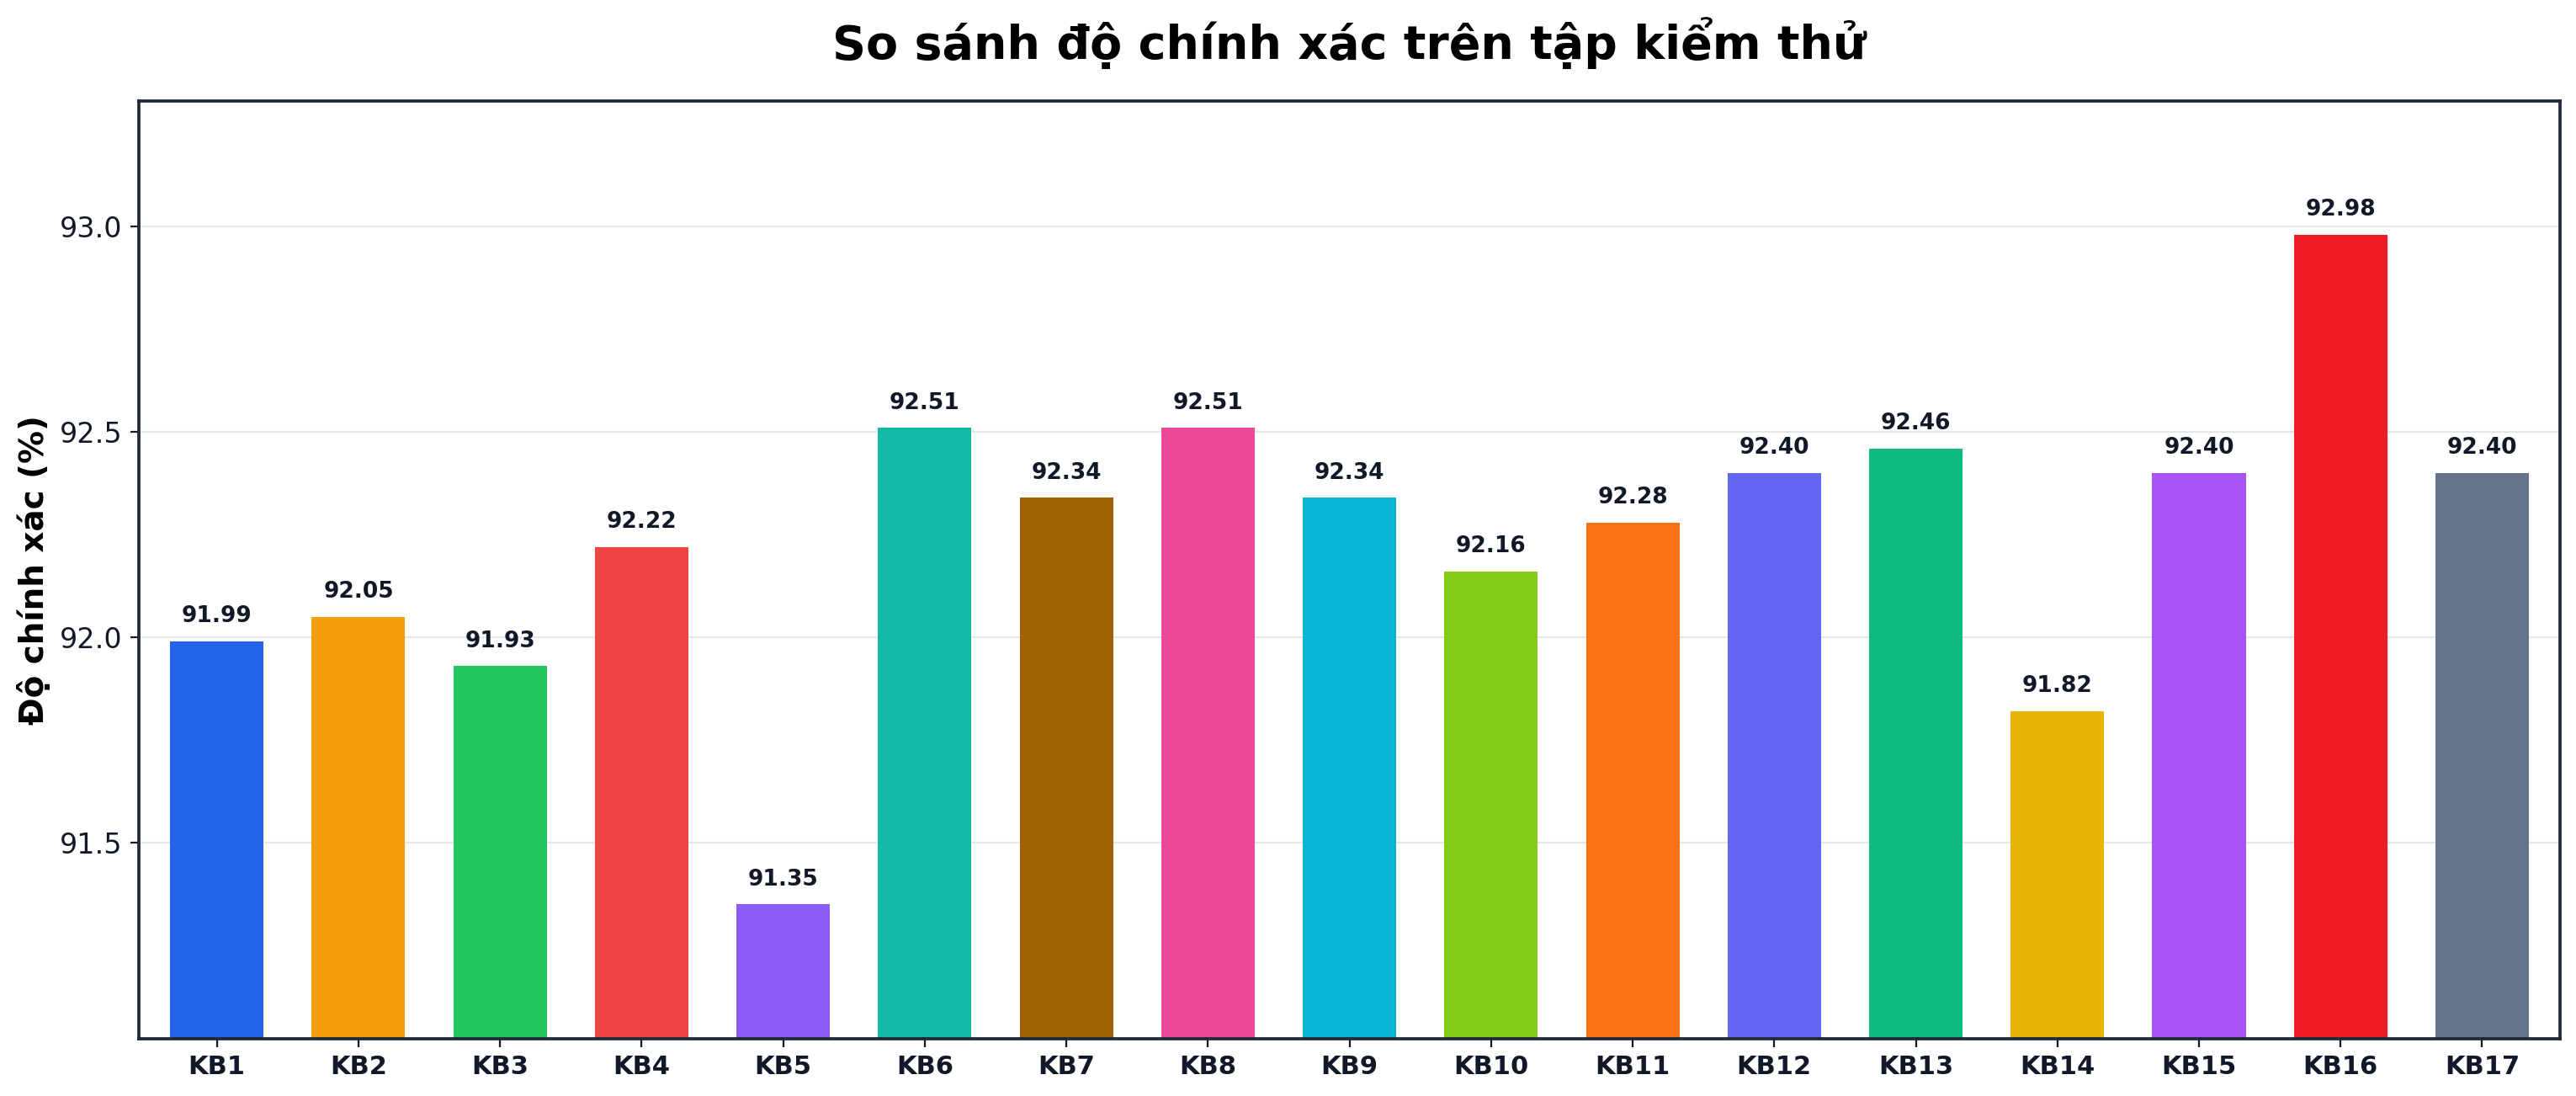
\includegraphics[width=\fairfigurewidth]{acc-loss/metric_accuracy_test_scenarios.png}
    \caption{Accuracy chart on the test set} 
    \label{tab:acc-test}
\end{figure}
Experimental results show that the Accuracy of the 17 models and fusion scenarios on the test set ranges from 91.35\% to 92.98\%. Overall, all models exceed 91\%, indicating relatively stable corporate credit-rating classification. Among individual models, T-LSTM achieves the highest result at 92.51\%, followed by GraphSAGE at 92.34\% and LSTM at 92.22\%. Tabular machine-learning models such as LightGBM and XGBoost also perform well, reaching 91.99\% and 92.05\%, respectively. Within the Fuzzy Ensemble group, FI-TTX achieves the highest Accuracy at 92.51\%, while FR-TTLPXL reaches 92.46\%, showing that fuzzy fusion methods maintain stable performance. Within the Dynamic Model Fusion group, DMF-TG achieves the best result in the entire chart, with 92.98\%. This result indicates that dynamic fusion among models can effectively exploit complementary information, particularly when combining a time-series model and a graph model.

\subsubsection{Confusion matrix}

\begingroup
\renewcommand{\arraystretch}{1.2}
\setlength{\tabcolsep}{4pt}
\begin{longtable}{>{\centering\arraybackslash}m{0.31\textwidth}
                   >{\centering\arraybackslash}m{0.31\textwidth}
                   >{\centering\arraybackslash}m{0.31\textwidth}}
\caption{Confusion matrices of the scenarios on the test set}
\label{tab:confusion_matrices}\\

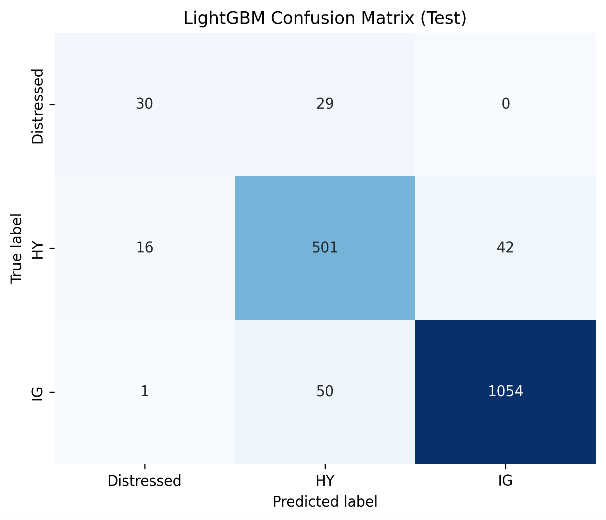
\includegraphics[width=0.95\linewidth]{acc-loss/confusion_lightgbm.png} &
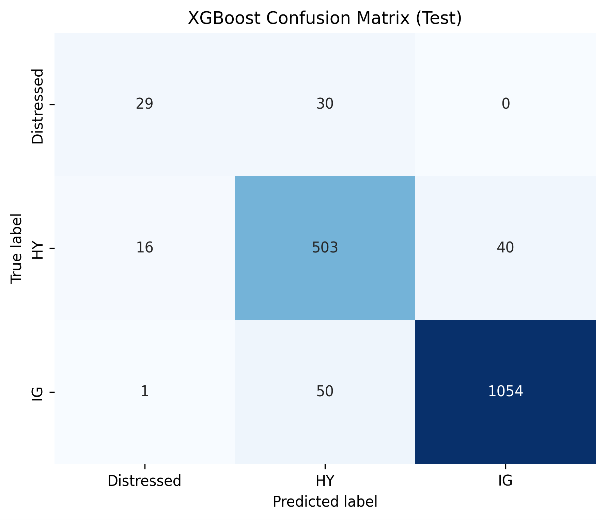
\includegraphics[width=0.95\linewidth]{acc-loss/confusion_xgboost.png} &
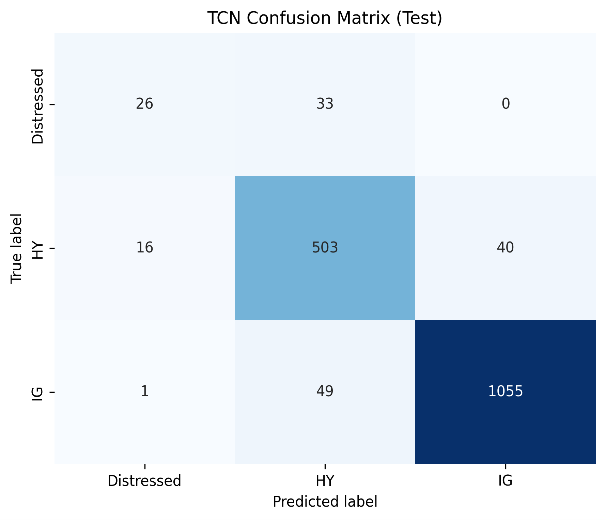
\includegraphics[width=0.95\linewidth]{acc-loss/confusion_tcn.png} \\


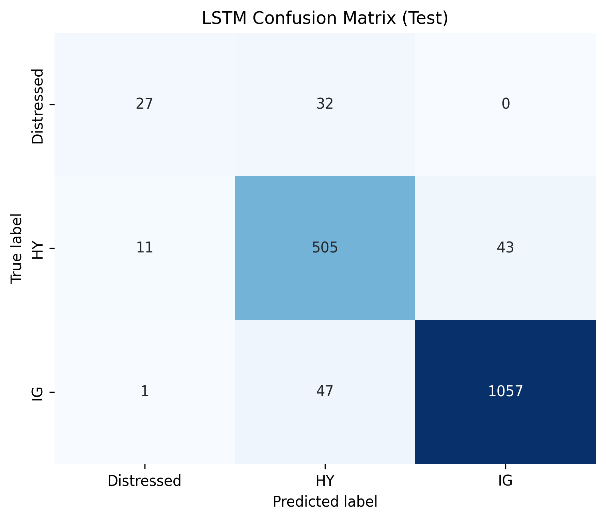
\includegraphics[width=0.95\linewidth]{acc-loss/confusion_lstm.png} &
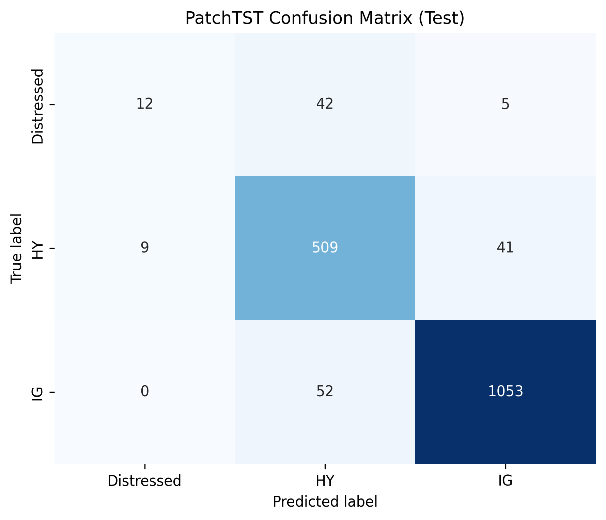
\includegraphics[width=0.95\linewidth]{acc-loss/confusion_patchtst.png} &
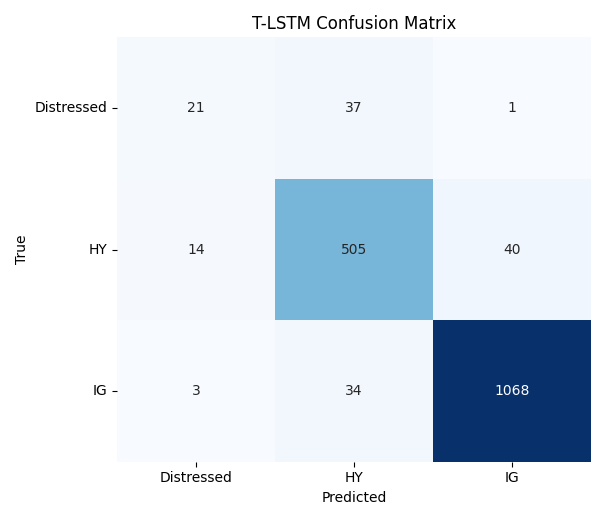
\includegraphics[width=0.95\linewidth]{acc-loss/confusion_tlstm.png} \\


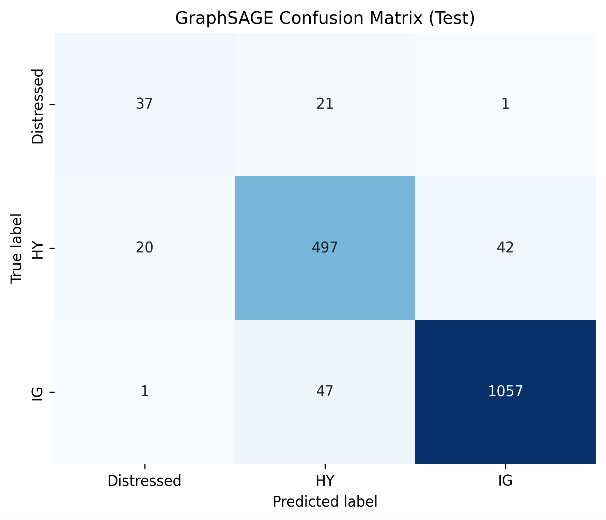
\includegraphics[width=0.95\linewidth]{acc-loss/confusion_graphsage.png} & 
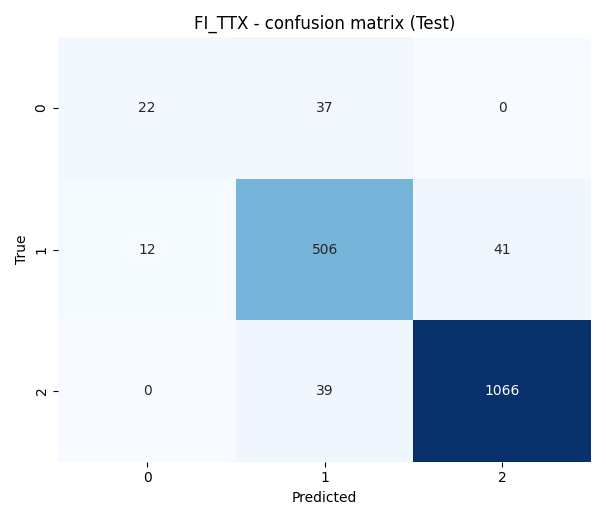
\includegraphics[width=0.95\linewidth]{acc-loss/confusion_fi_ttx.png} &
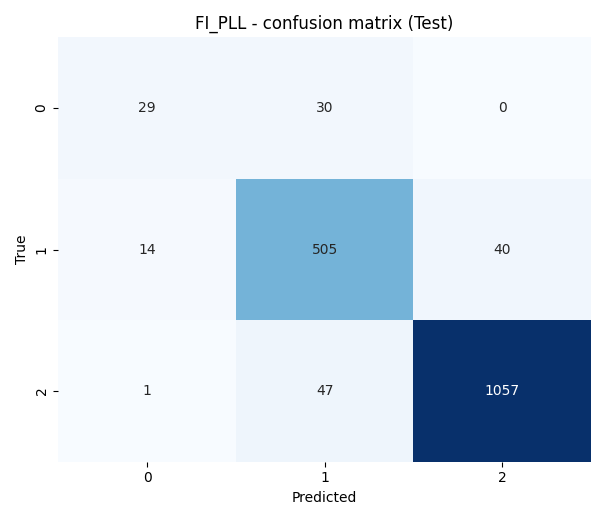
\includegraphics[width=0.95\linewidth]{acc-loss/confusion_fi_pll.png} \\


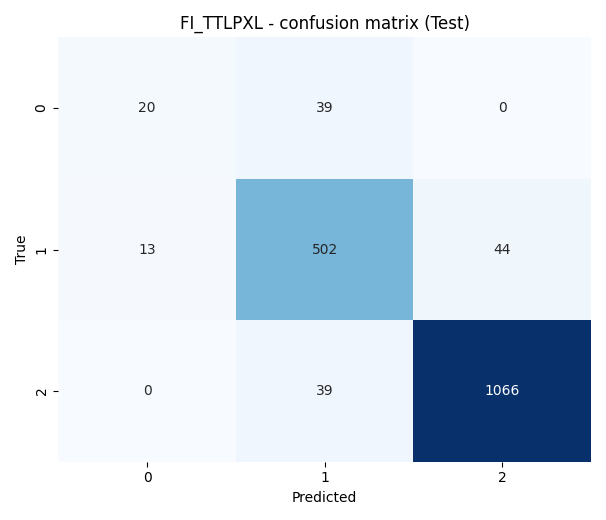
\includegraphics[width=0.95\linewidth]{acc-loss/confusion_fi_ttlpxl.png} & 
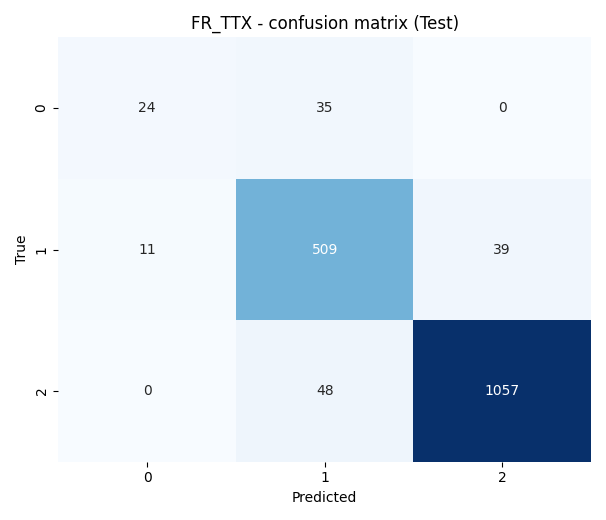
\includegraphics[width=0.95\linewidth]{acc-loss/confusion_fr_ttx.png} &
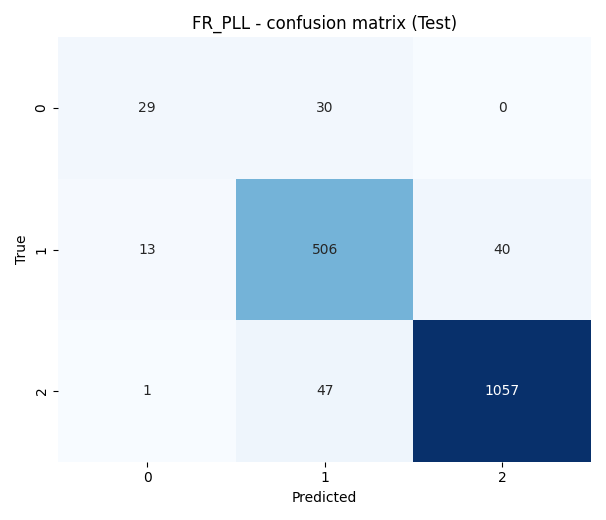
\includegraphics[width=0.95\linewidth]{acc-loss/confusion_fr_pll.png} \\


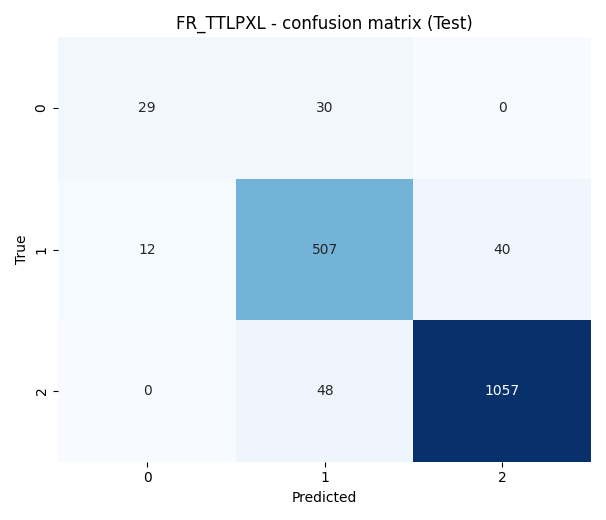
\includegraphics[width=0.95\linewidth]{acc-loss/confusion_fr_ttlpxl.png} &
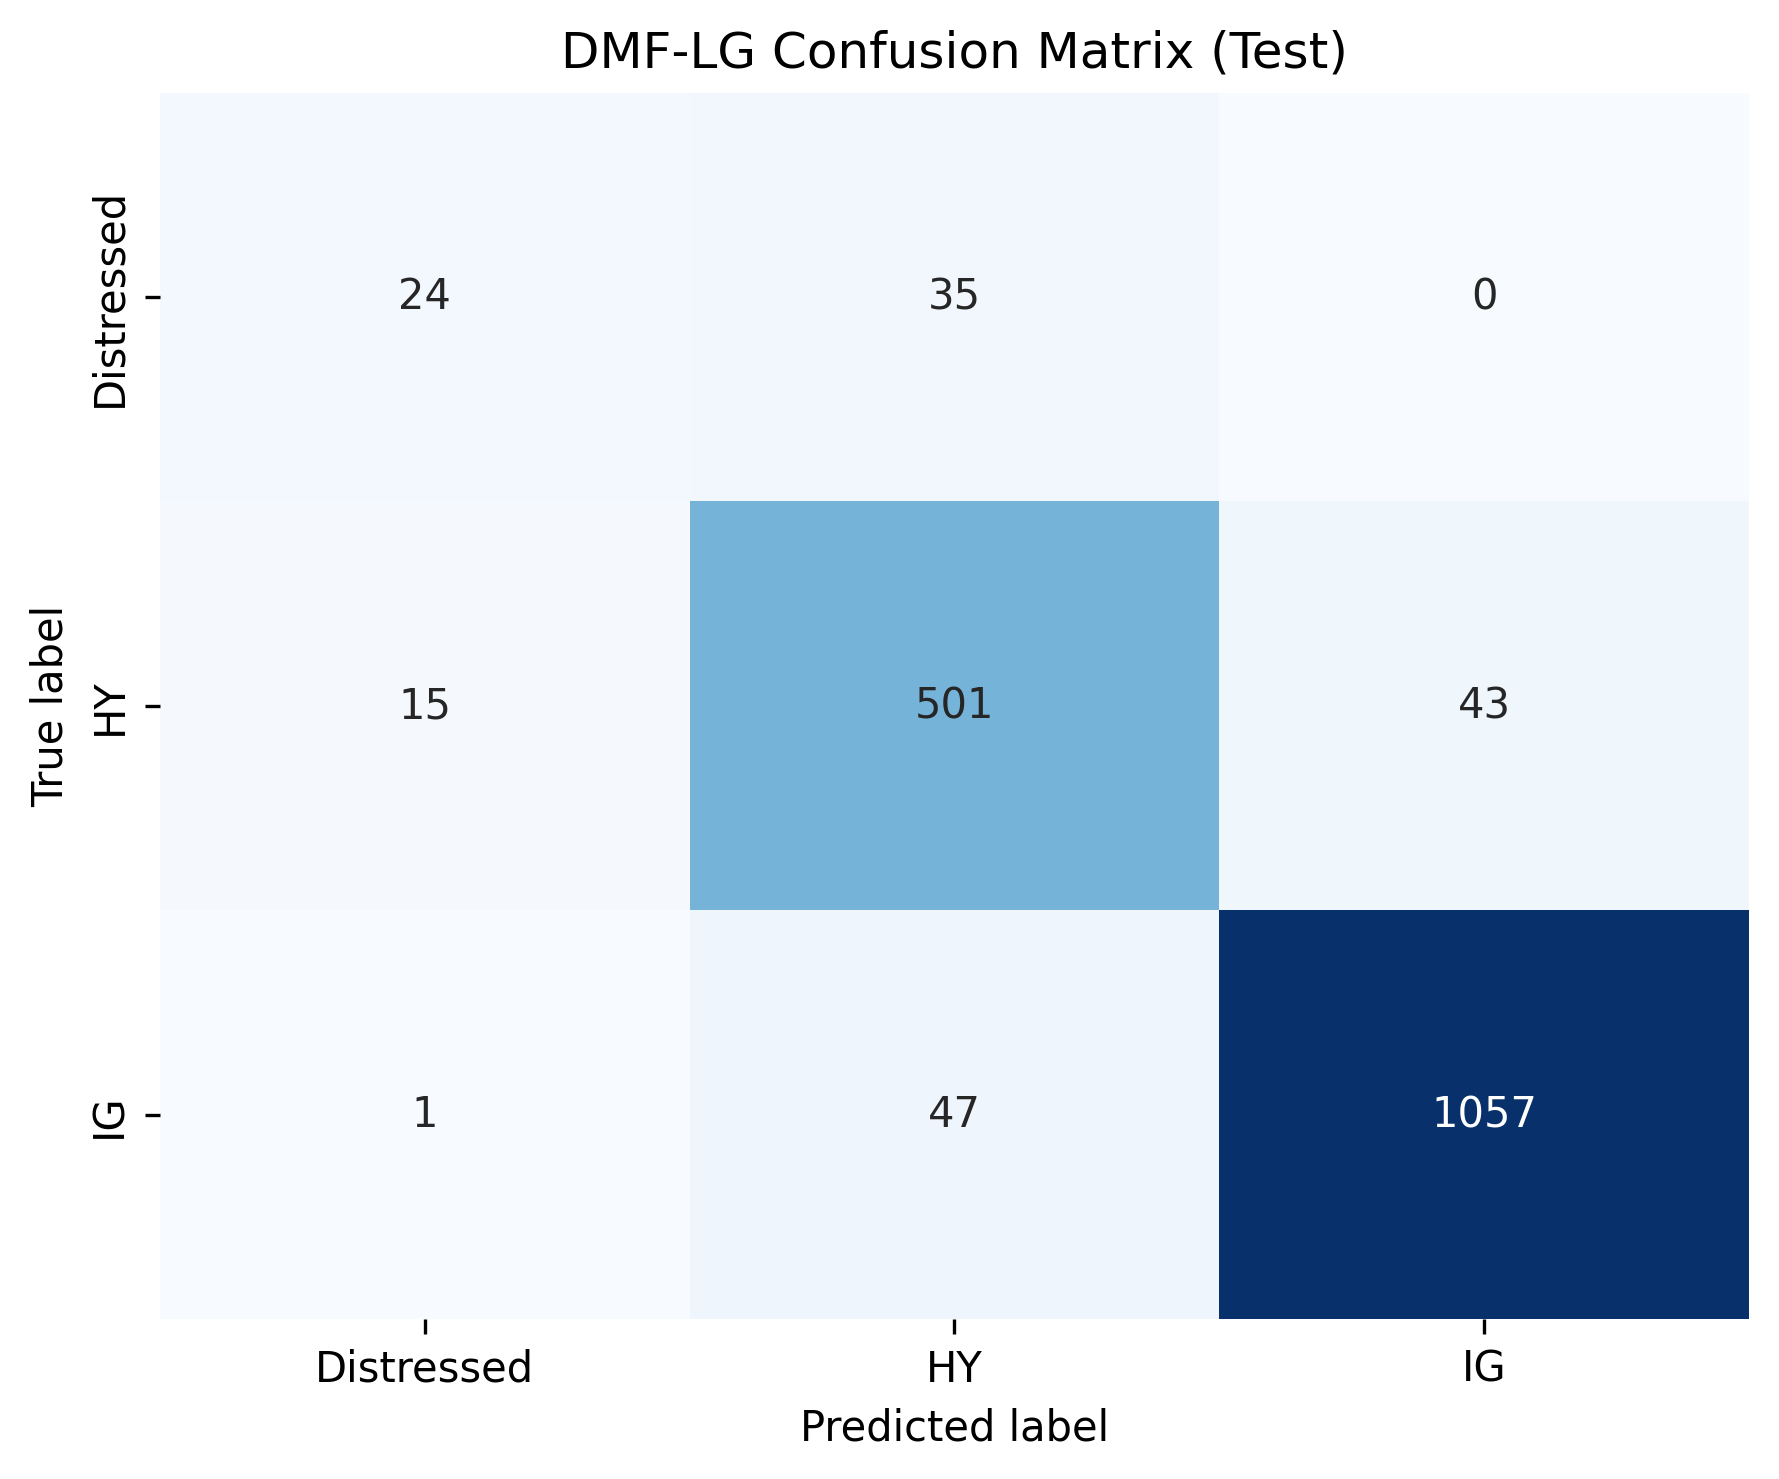
\includegraphics[width=0.95\linewidth]{acc-loss/confusion_dmf_lstm_graphsage.png} & 
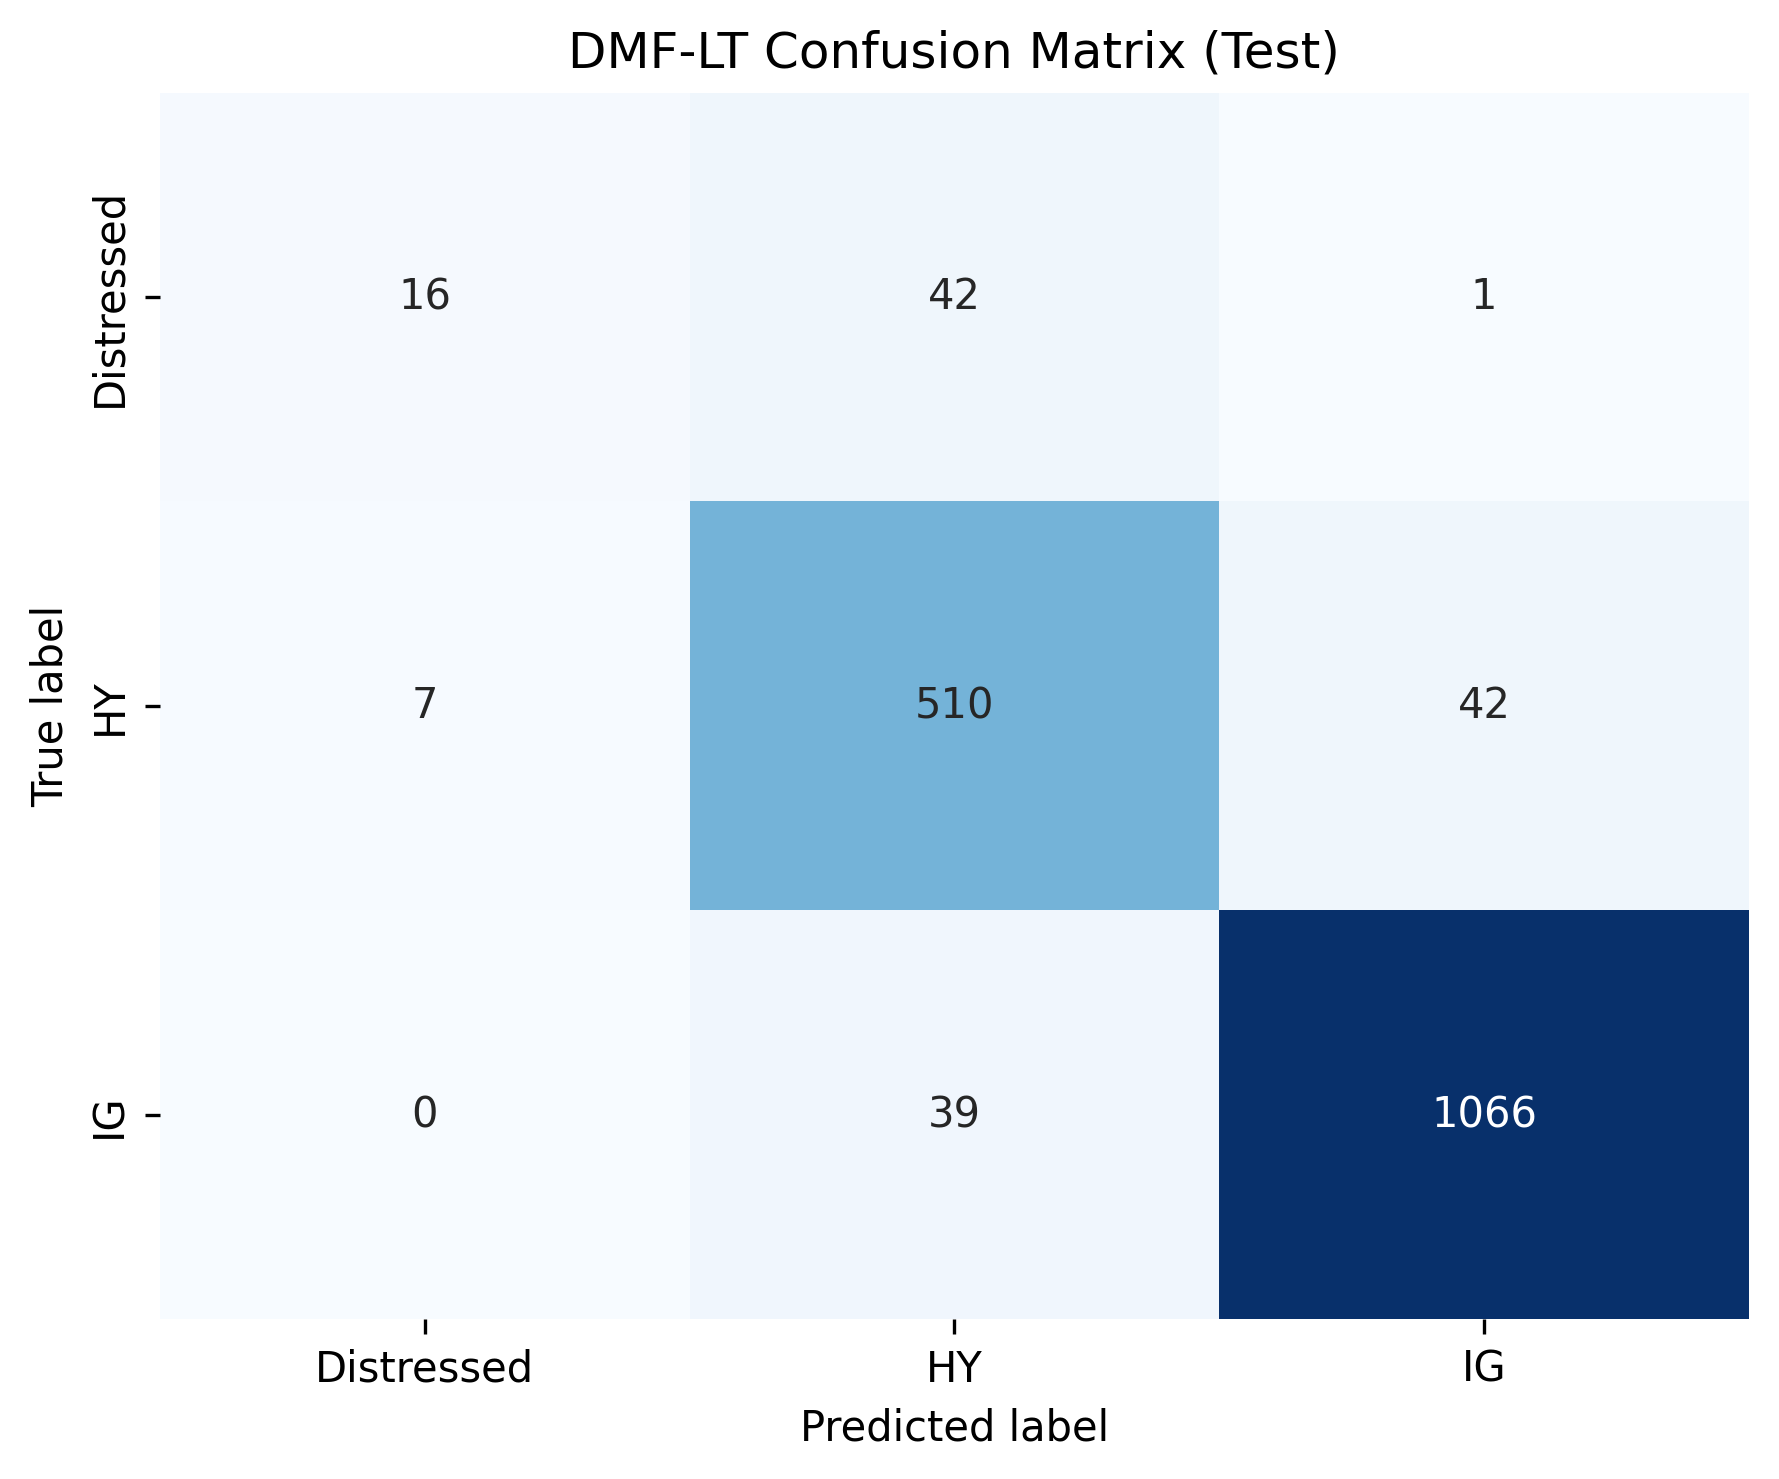
\includegraphics[width=0.95\linewidth]{acc-loss/confusion_dmf_lstm_tlstm.png} \\

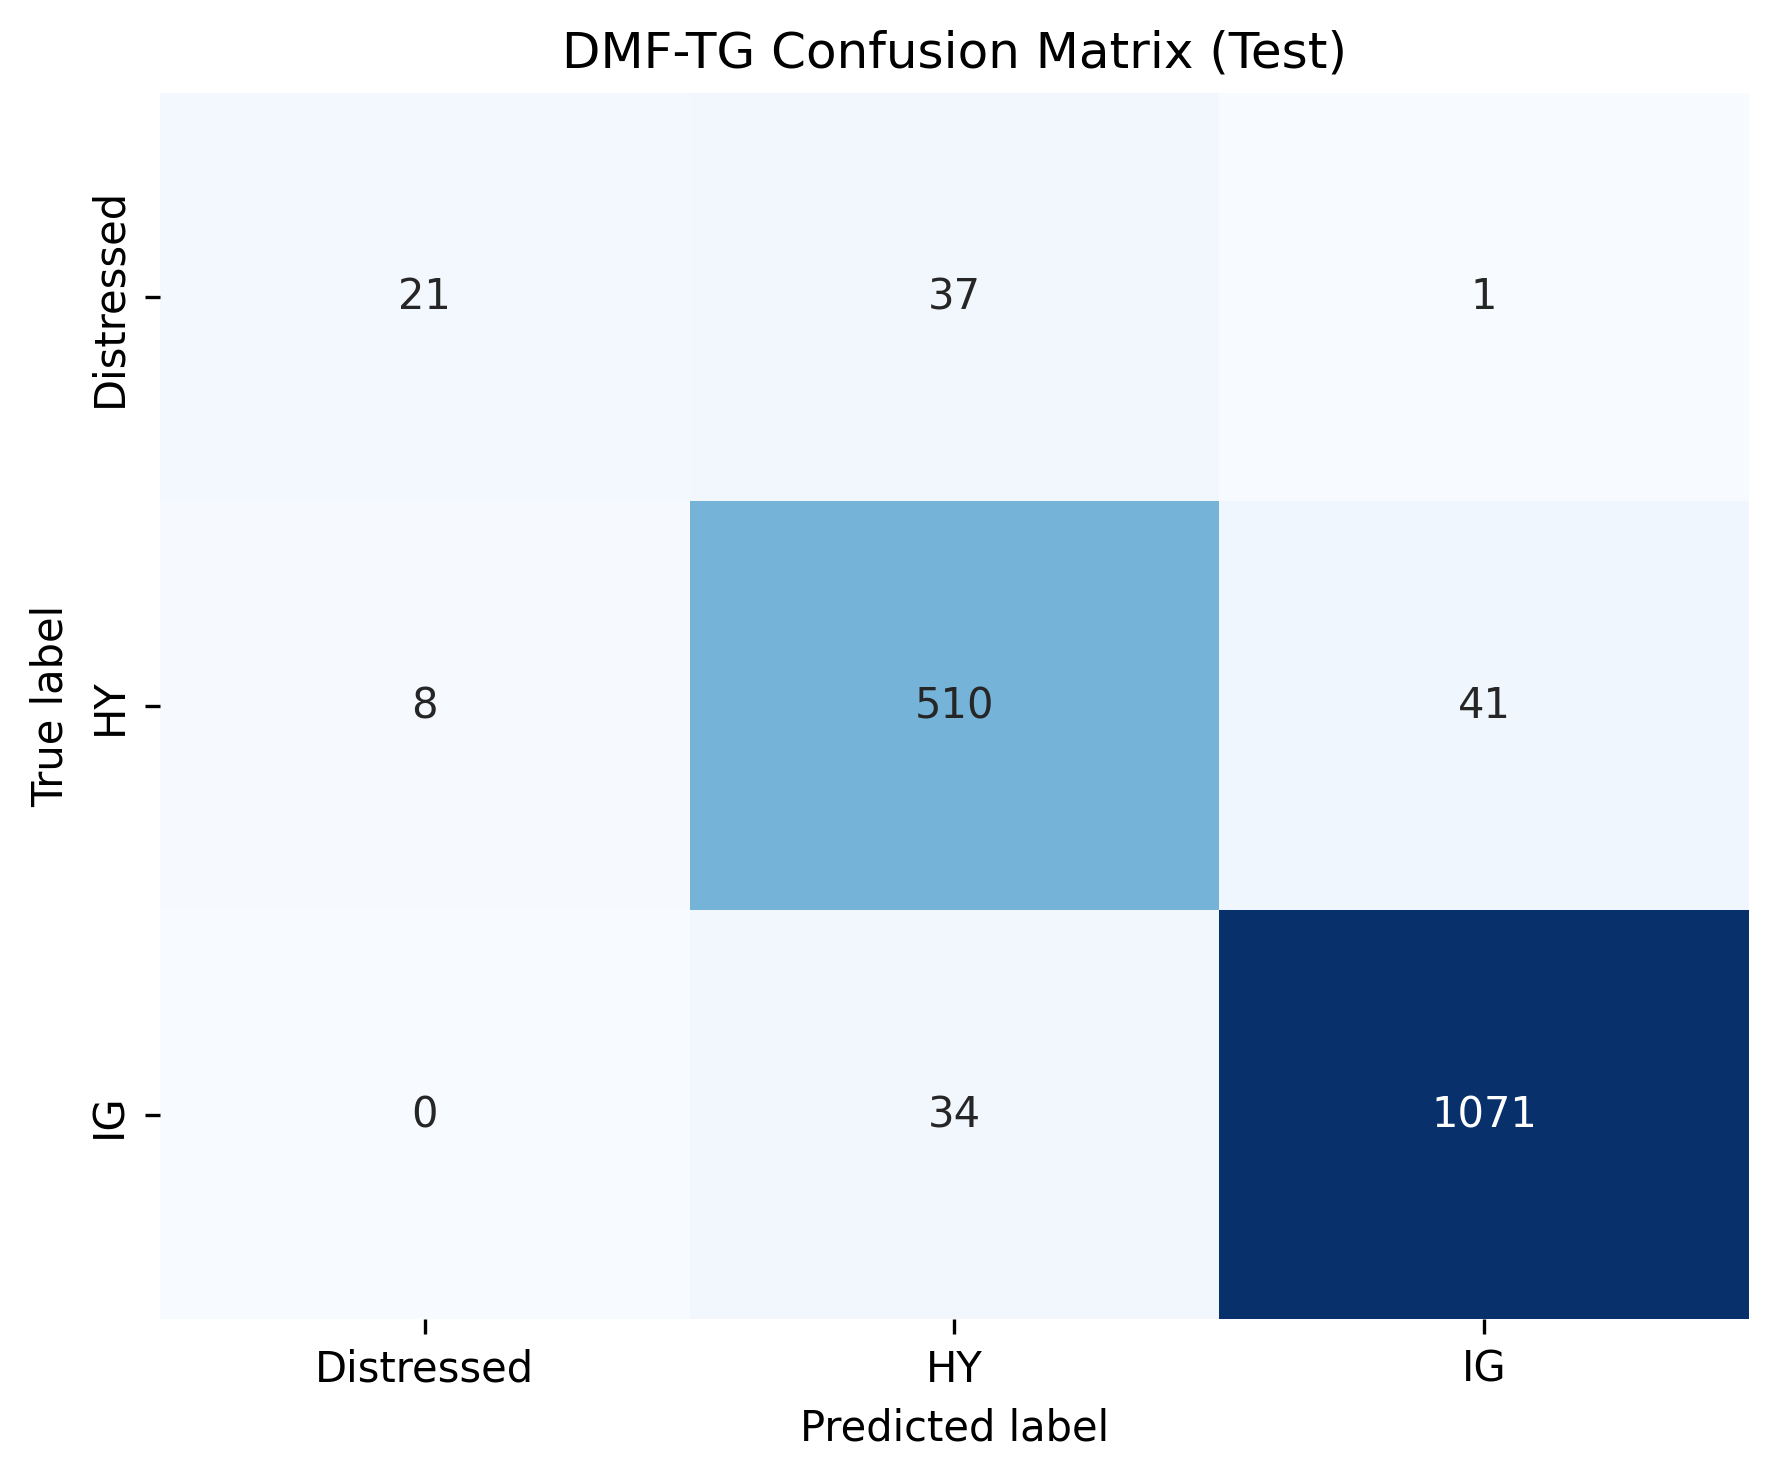
\includegraphics[width=0.95\linewidth]{acc-loss/confusion_dmf_tlstm_graphsage.png} &
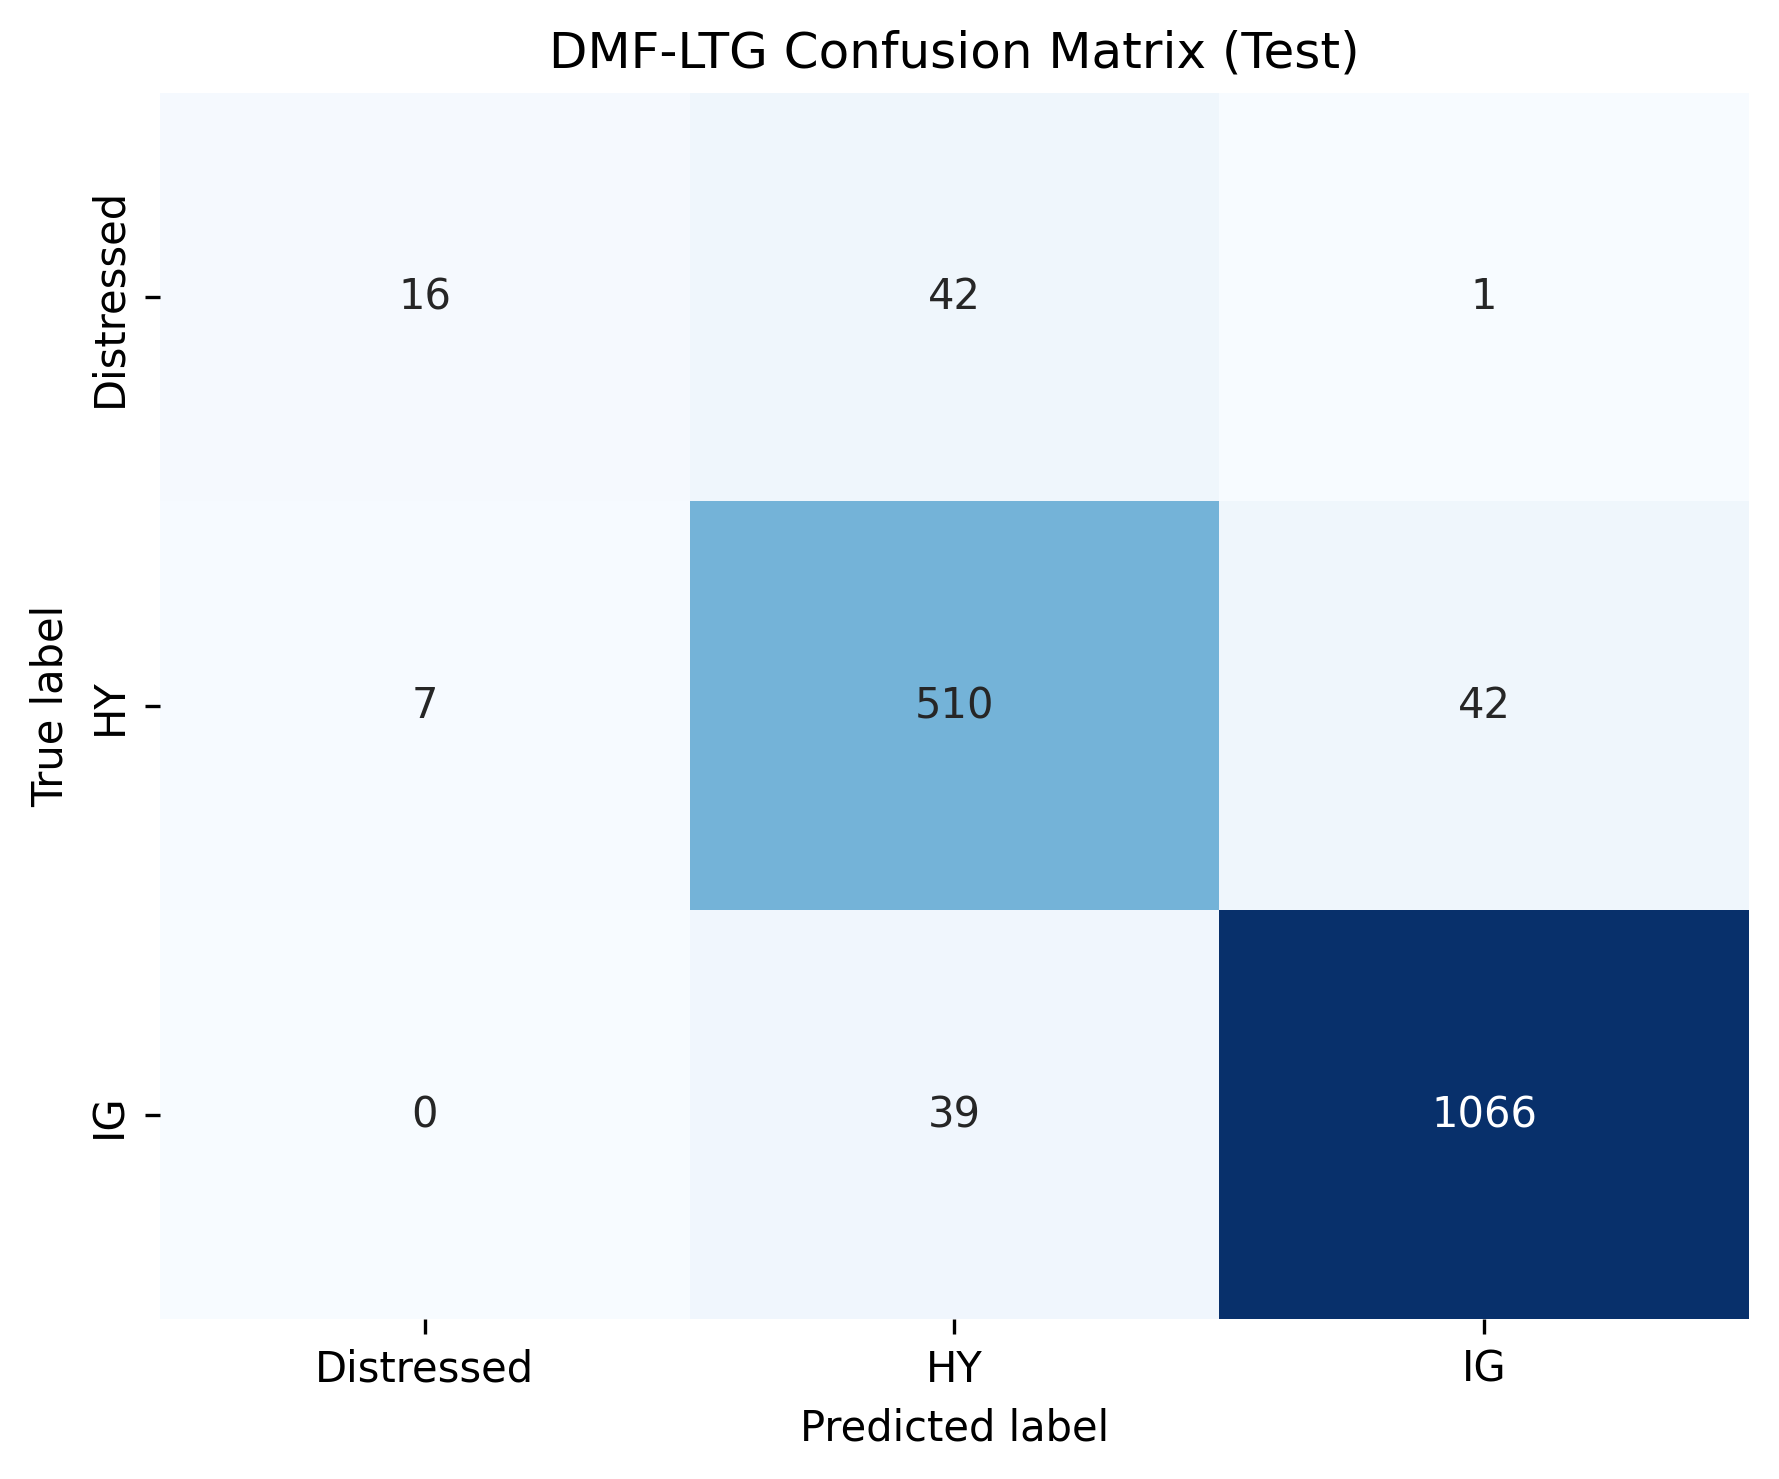
\includegraphics[width=0.95\linewidth]{acc-loss/confusion_dmf_lstm_tlstm_graphsage.png} & \\
\end{longtable}
\endgroup

The confusion matrices on the test set show that the models generally classify the HY and IG classes well.
Among them, IG is the most stably identified class, with a high number of correct predictions in most scenarios.
This indicates that firms with strong credit quality tend to have clearer financial characteristics.
By contrast, Distressed is the most difficult class for all models to identify.
The most common error is that Distressed samples are misclassified as HY, reflecting the fact that the boundary between these two groups is not fully clear.
However, the number of Distressed samples directly misclassified as IG is very low, indicating that the models still distinguish well between two distant risk levels.
Among individual models, GraphSAGE has an advantage for the Distressed class because it correctly predicts more high-risk samples than other models.
T-LSTM performs well for the IG class, showing its ability to learn time-series features of stable firms.
Fuzzy Ensemble scenarios help maintain stable results for HY and IG but do not clearly improve Distressed-class recognition.
Within the DMF group, DMF-TG is the most prominent scenario, achieving the highest number of correctly predicted IG samples and strong overall performance.
The DMF group shows an advantage in improving overall Accuracy, especially for HY and IG.
However, if the objective is early detection of high-risk firms, the ability to identify the Distressed class still needs further improvement.

\subsubsection{Precision of the scenarios}

\begin{figure}[H]
\centering
\setupfairsubfigures
\begin{subfigure}{\fairfigurewidth}
    \centering
    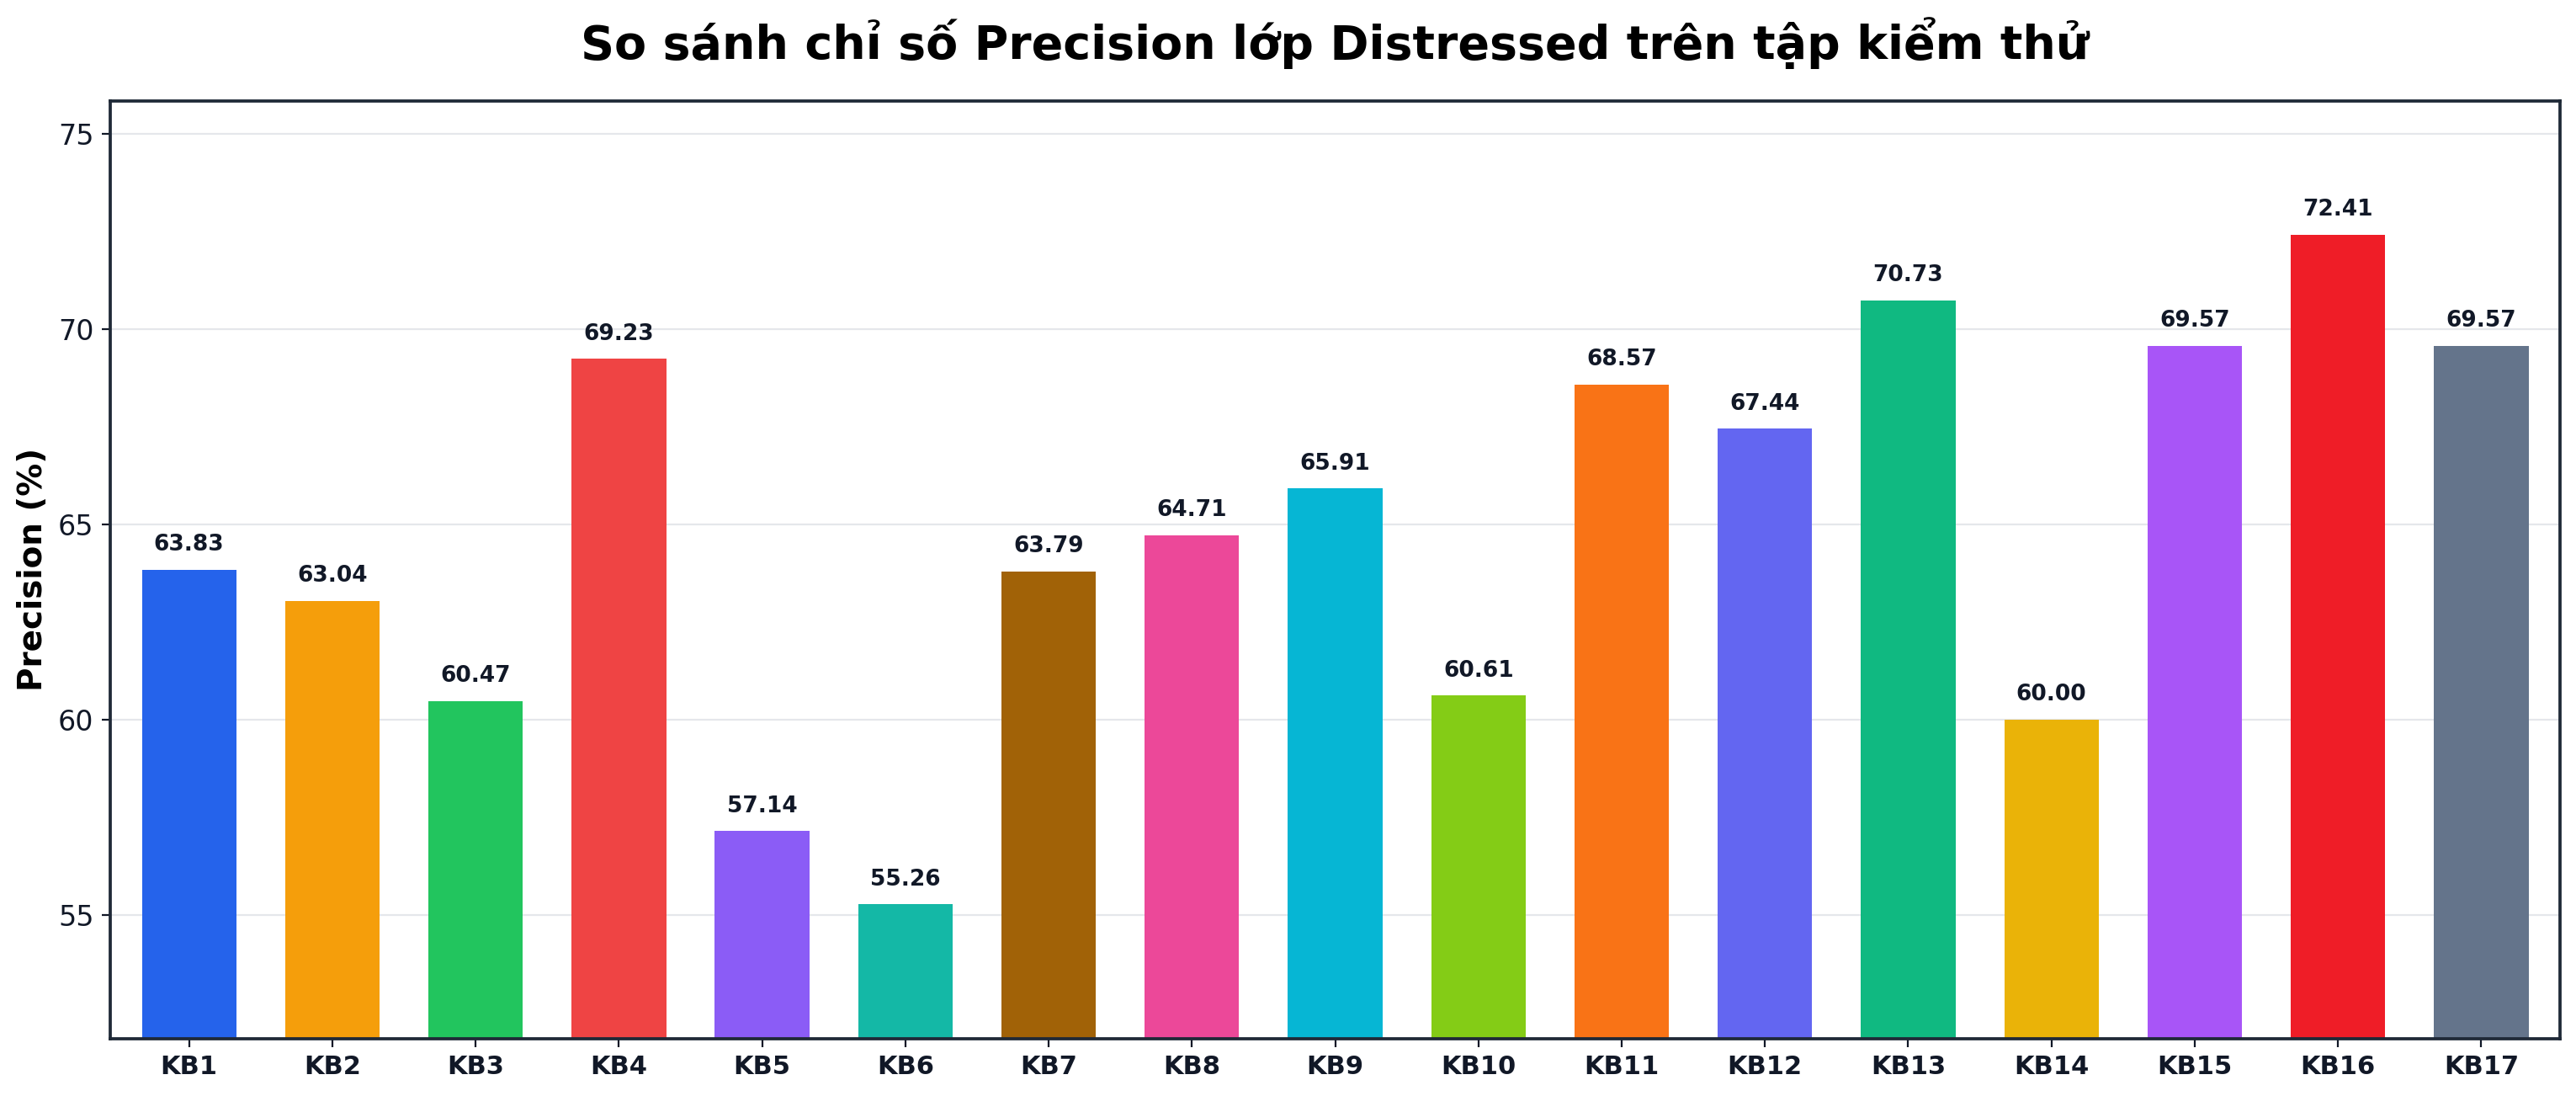
\includegraphics[width=\textwidth]{acc-loss/metric_precision_distressed_test.png}
    \caption{Precision of the Distressed class}
    \label{fig:precision_distressed}
\end{subfigure}
\end{figure}

\begin{figure}[H]
\ContinuedFloat
\centering
\begin{subfigure}{\fairfigurewidth}
    \centering
    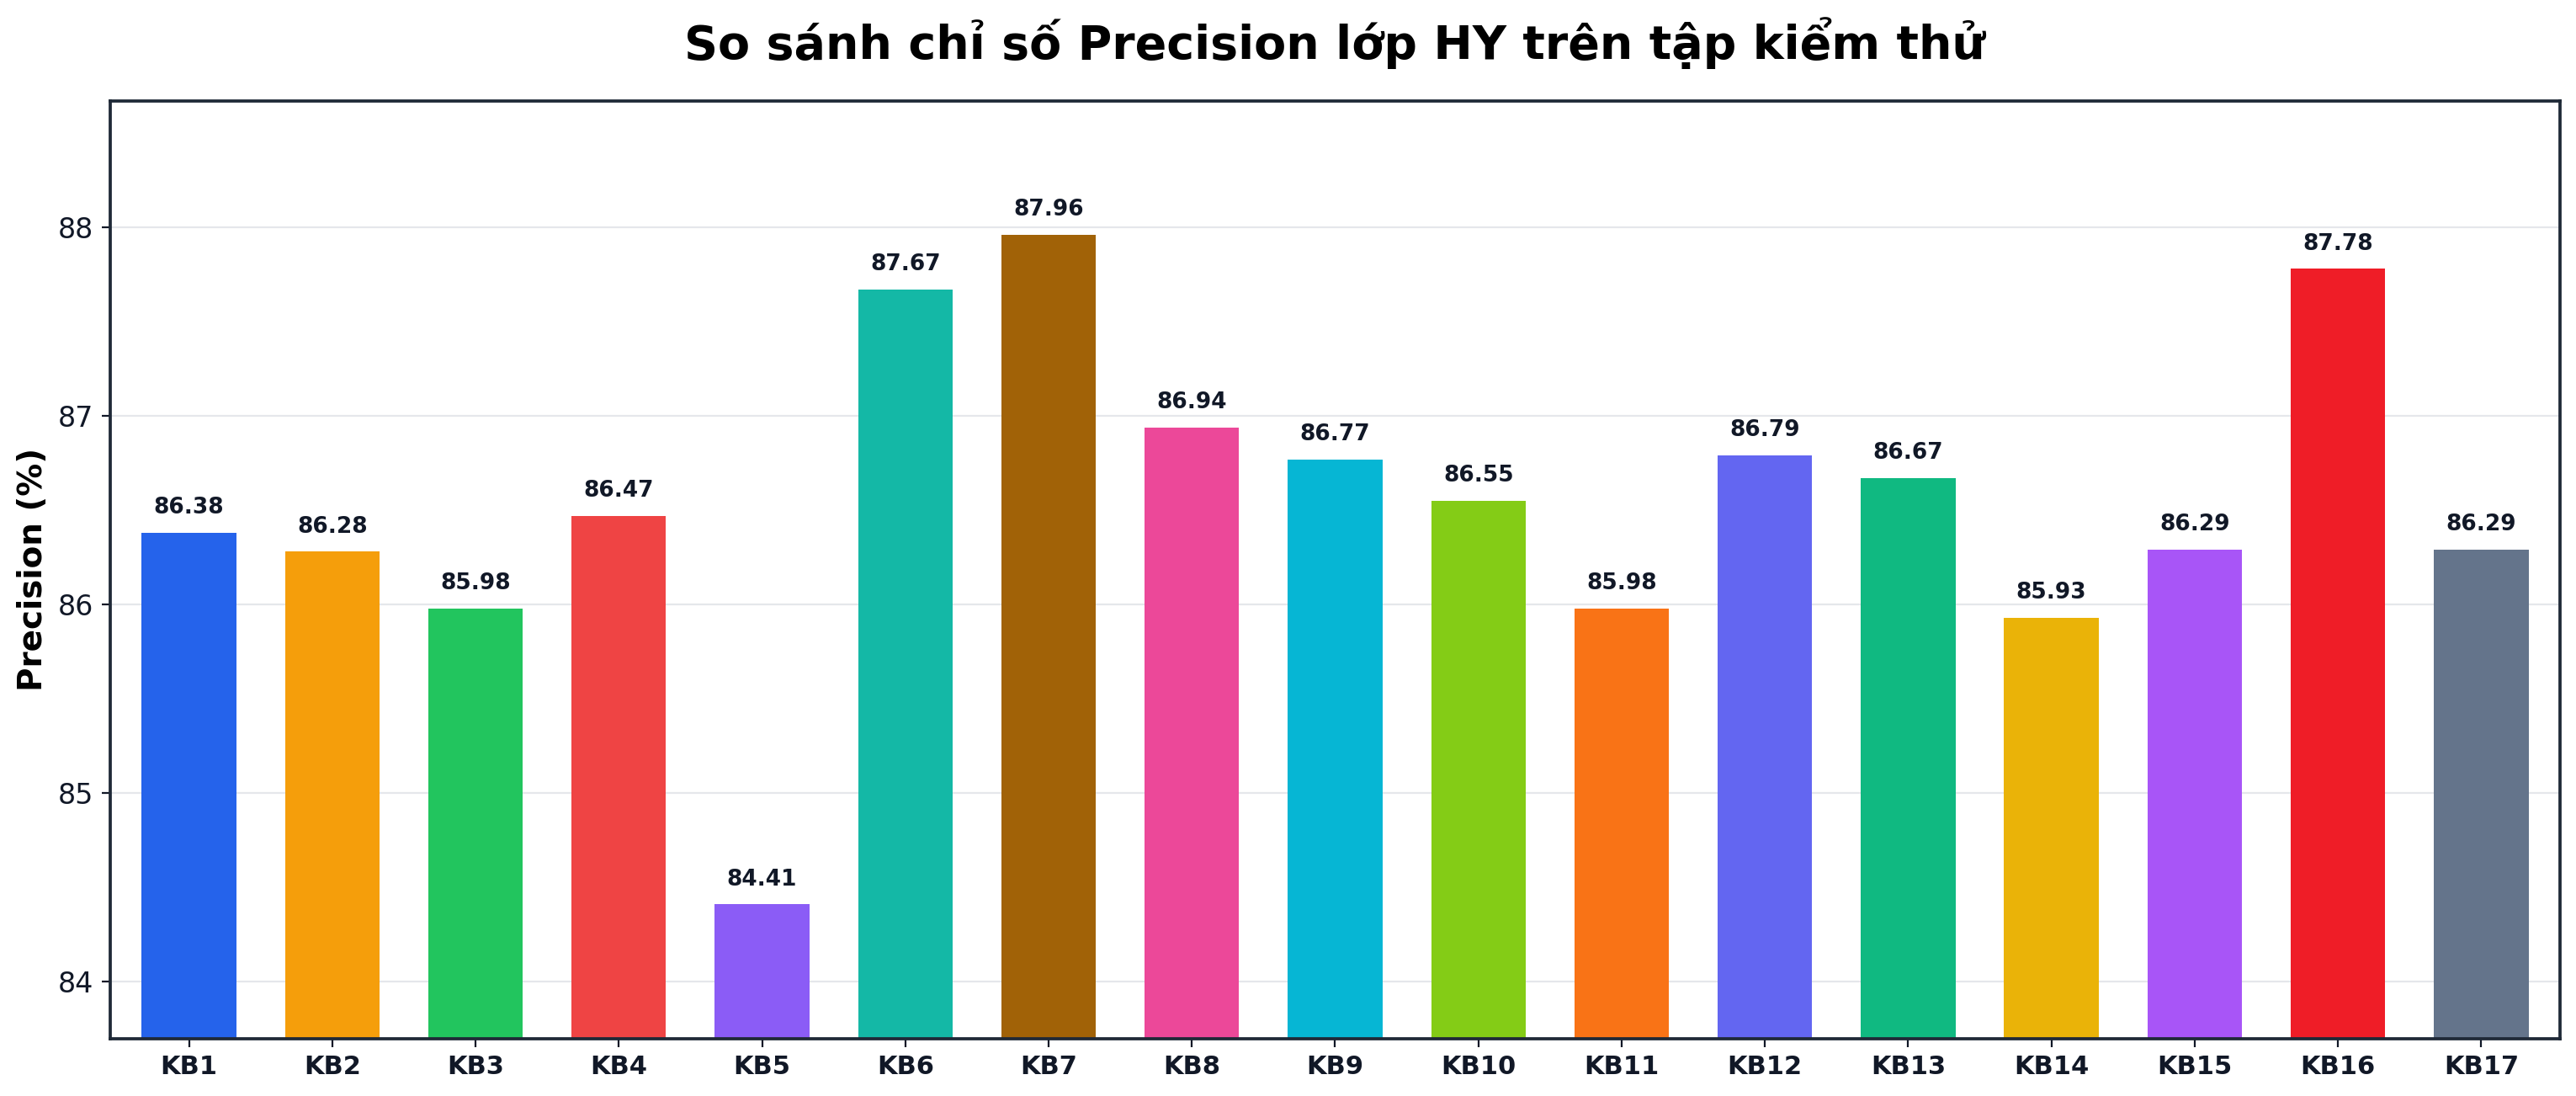
\includegraphics[width=\textwidth]{acc-loss/metric_precision_hy_test.png}
    \caption{Precision of the HY (High Yield) class}
    \label{fig:precision_hy}
\end{subfigure}

\end{figure}

\begin{figure}[H]
\ContinuedFloat
\centering
\begin{subfigure}{\fairfigurewidth}
    \centering
    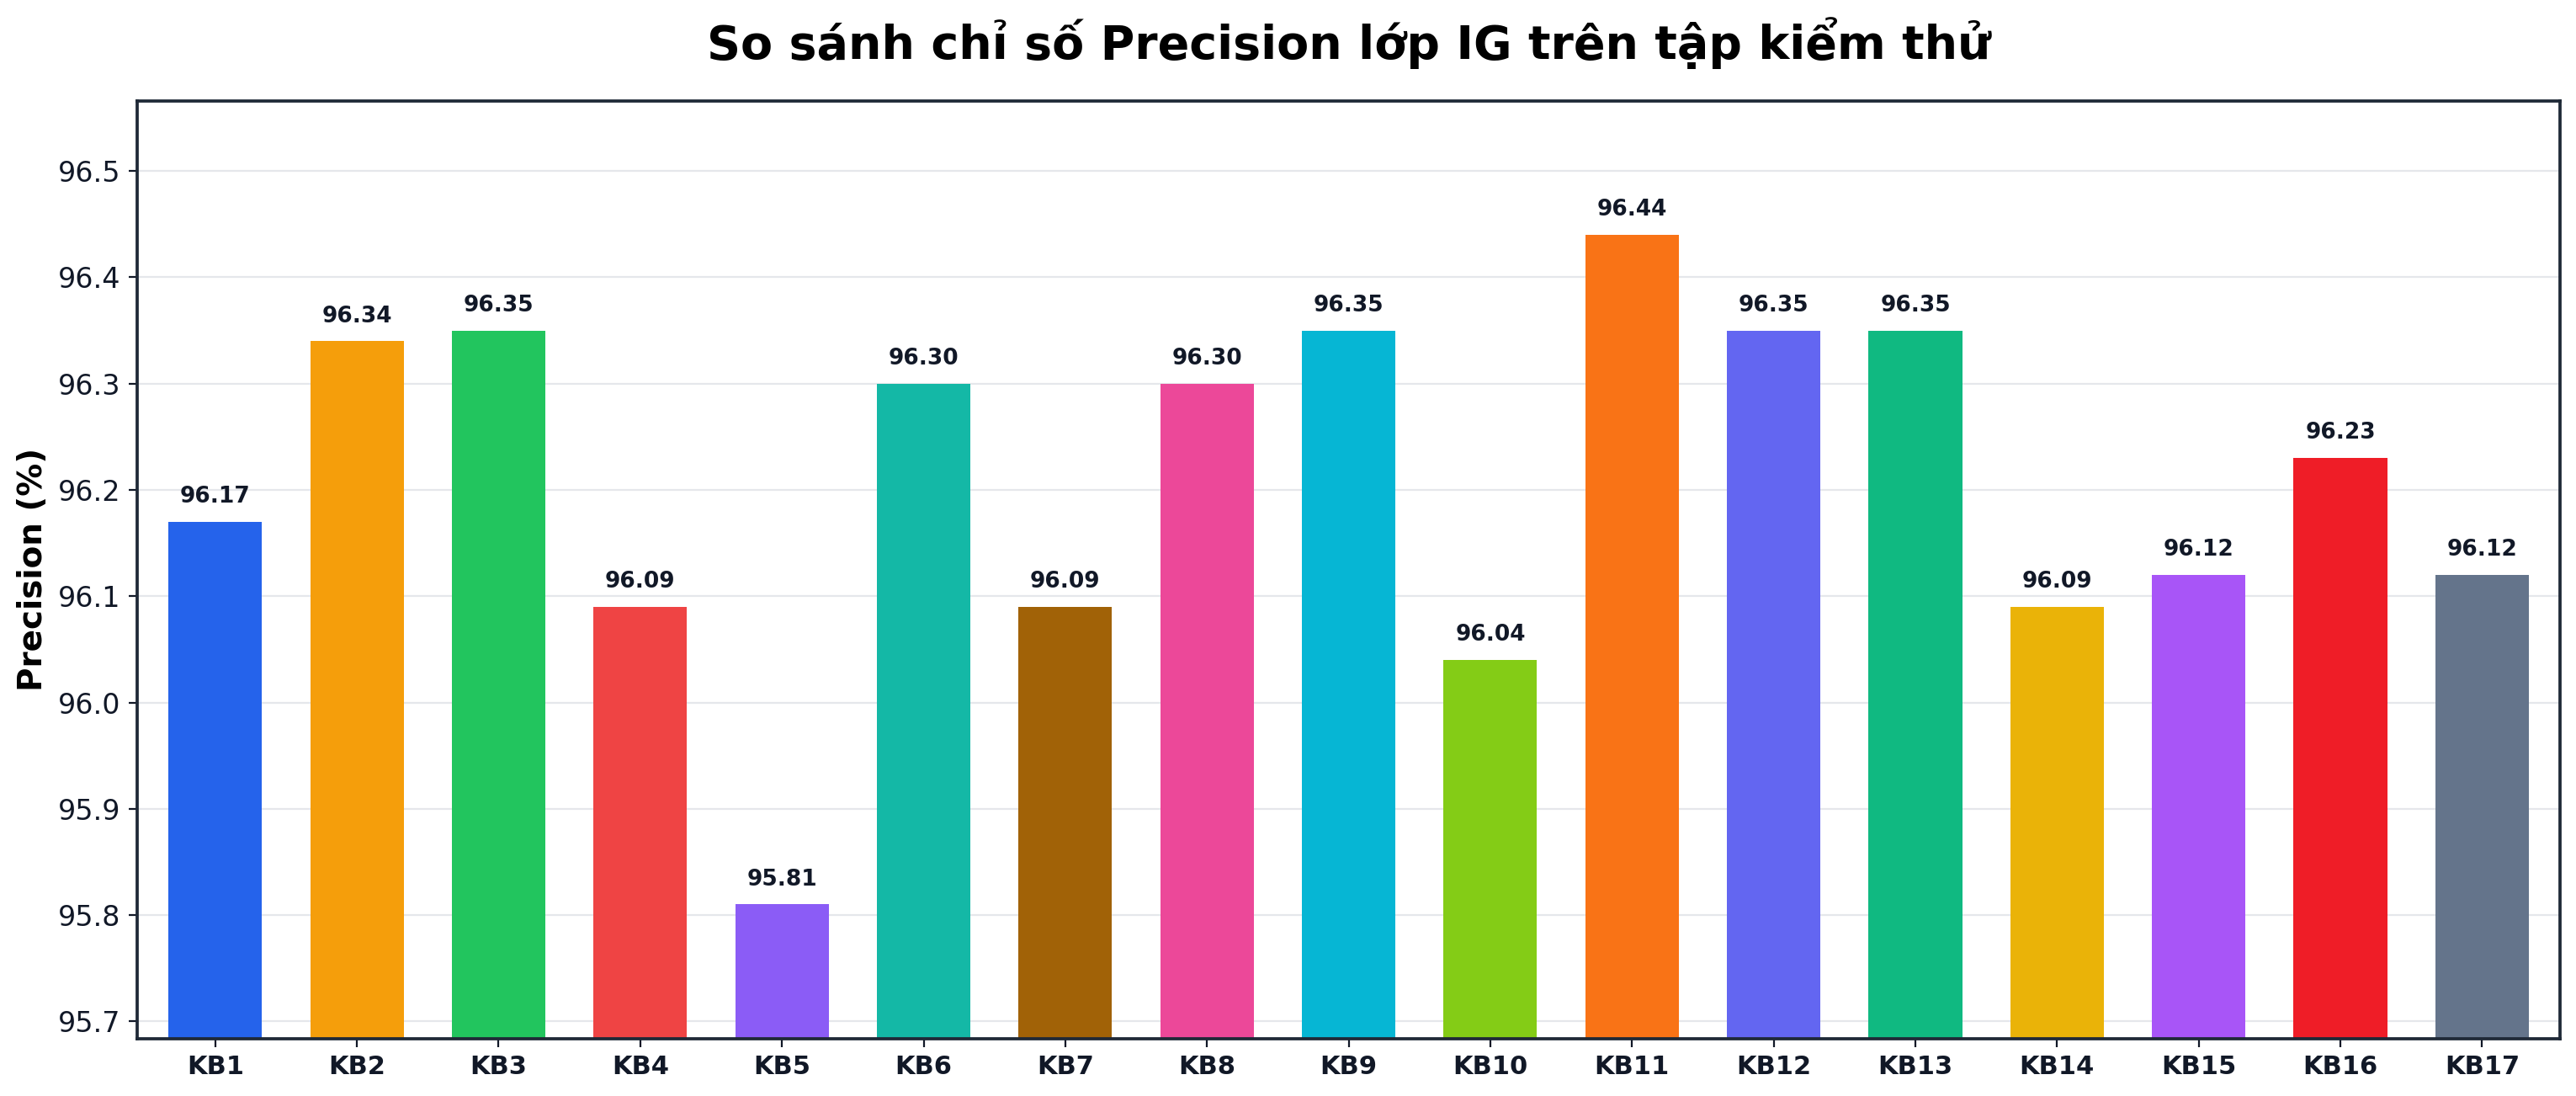
\includegraphics[width=\textwidth]{acc-loss/metric_precision_ig_test.png}
    \caption{Precision of the IG (Investment Grade) class}
    \label{fig:precision_ig}
\end{subfigure}
\caption{Precision of the Distressed (a), HY (b), and IG (c) classes on the test set}
\label{fig:precision_classes}
\end{figure}

Precision results on the test set show that prediction effectiveness differs across the three credit-rating classes.
The IG class achieves the highest and most stable Precision, mainly around 96\%, indicating strong recognition of firms with high credit quality.
The HY class also shows relatively consistent results, ranging from 84.41\% to 87.96\%. GraphSAGE achieves the highest Precision for HY at 87.96\%, followed by DMF-TG and T-LSTM. In contrast, Distressed is the most difficult class to classify because of its small sample size and ambiguous boundary with HY.
Among individual models, LSTM achieves the highest Precision for Distressed at 69.23\%. Within the Fuzzy Ensemble group, FR-TTLPXL obtains the best Distressed-class result at 70.73\%. Notably, DMF-TG achieves the highest Distressed-class Precision in the entire chart at 72.41\%. This indicates that dynamically combining T-LSTM and GraphSAGE improves the recognition of high-risk firms. Overall, DMF-TG is the most prominent scenario because it improves Precision for Distressed while maintaining strong performance for HY and IG.

\subsubsection{Recall of the scenarios}
\begin{figure}[H]
\centering
\setupfairsubfigures
\begin{subfigure}{\fairfigurewidth}
    \centering
    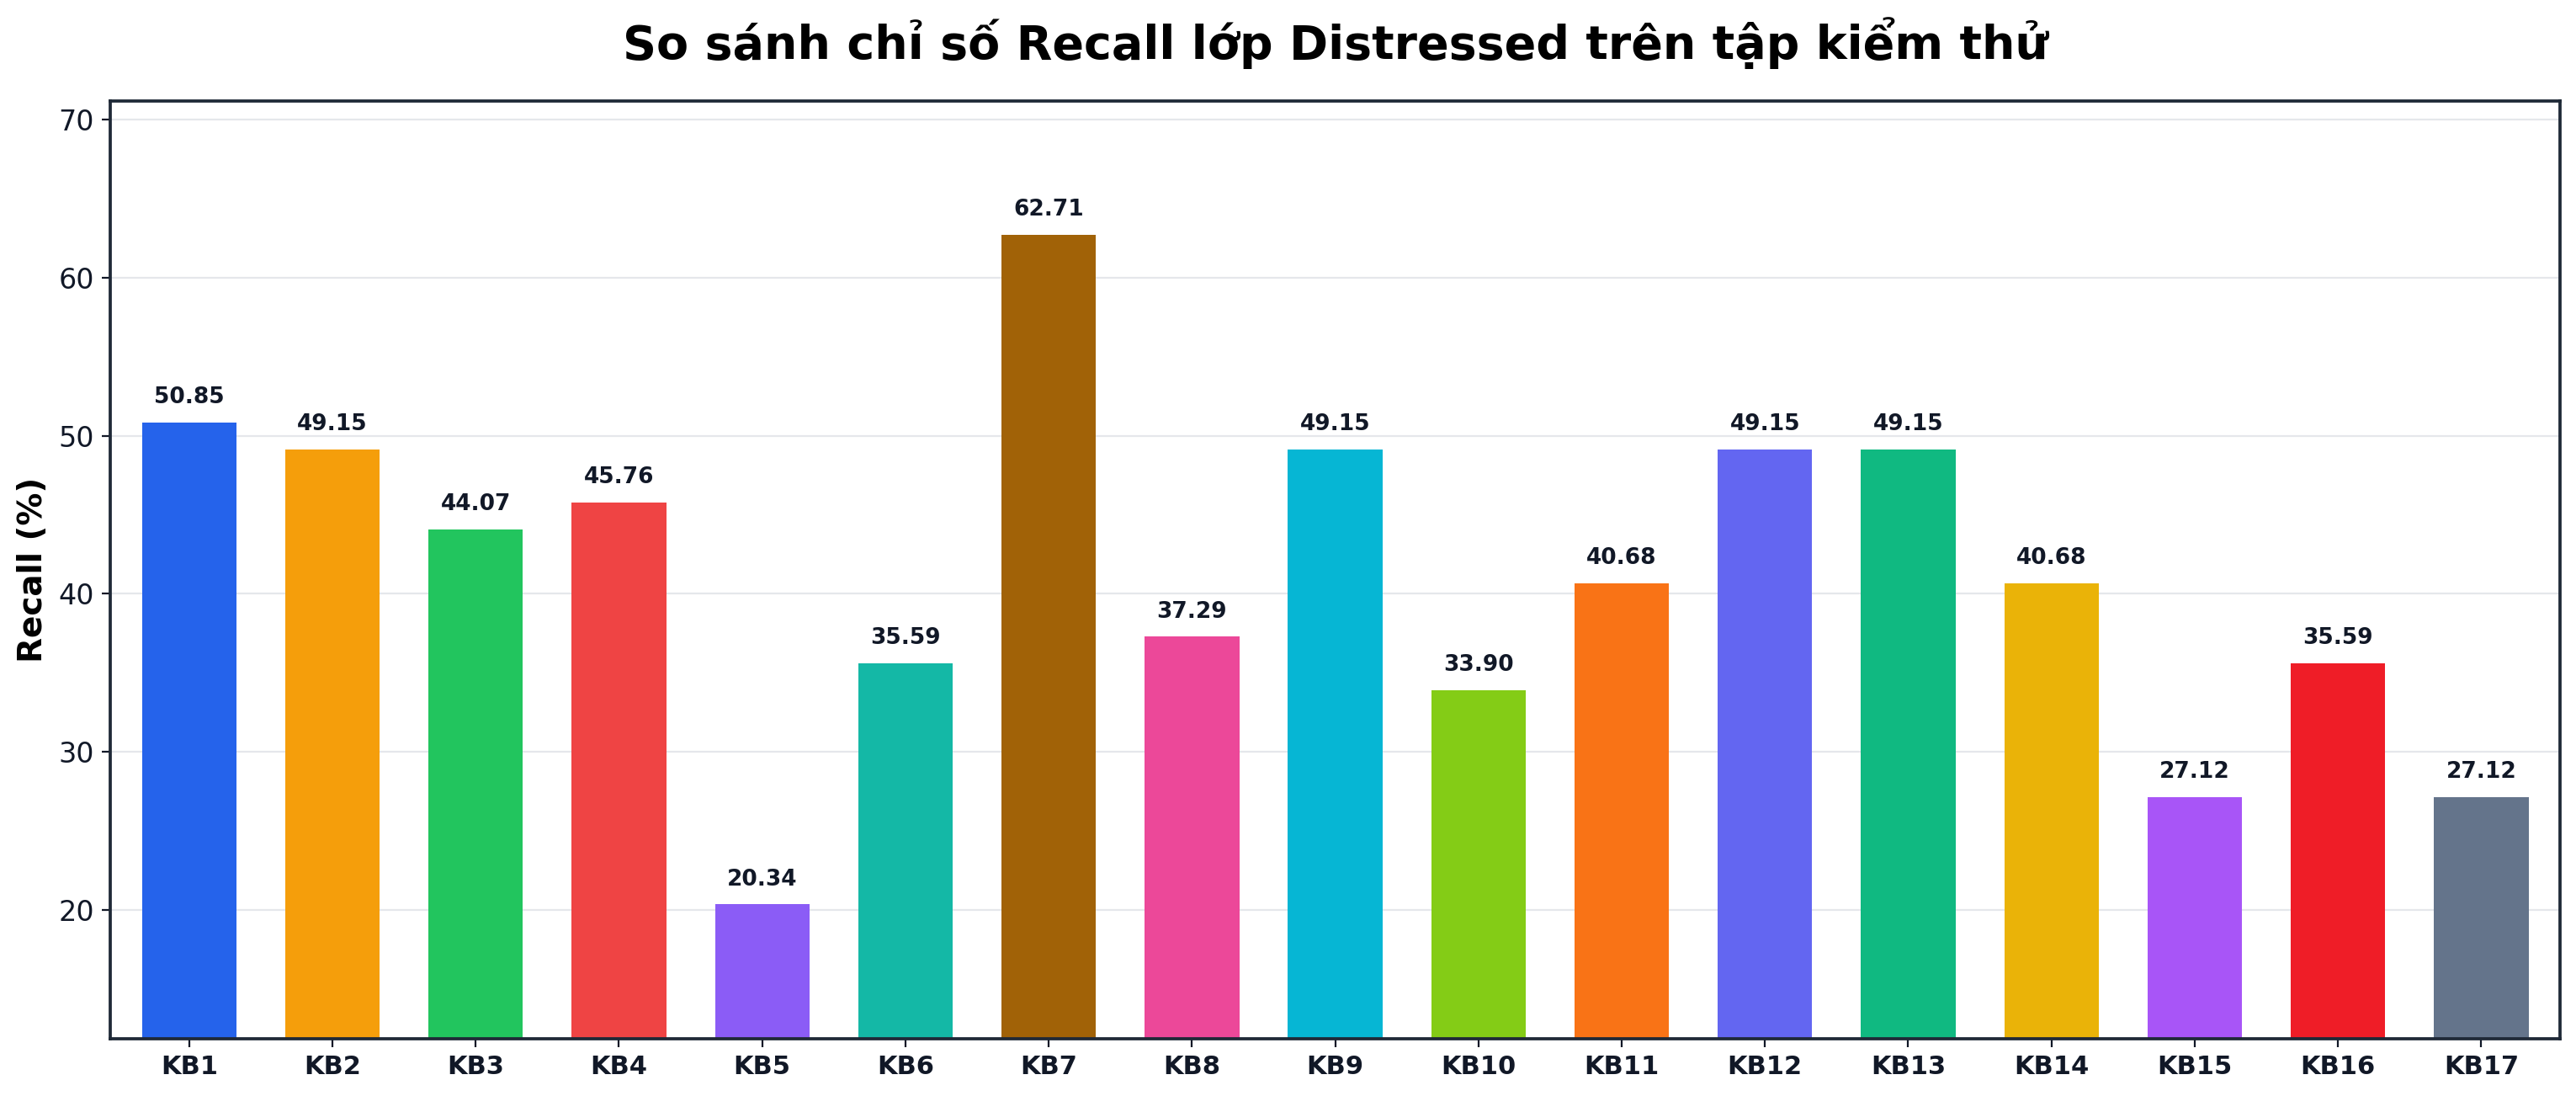
\includegraphics[width=\textwidth]{acc-loss/metric_recall_distressed_test.png}
    \caption{Recall of the Distressed class}
    \label{fig:Recall_distressed}
\end{subfigure}
\end{figure}

\begin{figure}[H]
\ContinuedFloat
\centering
\begin{subfigure}{\fairfigurewidth}
    \centering
    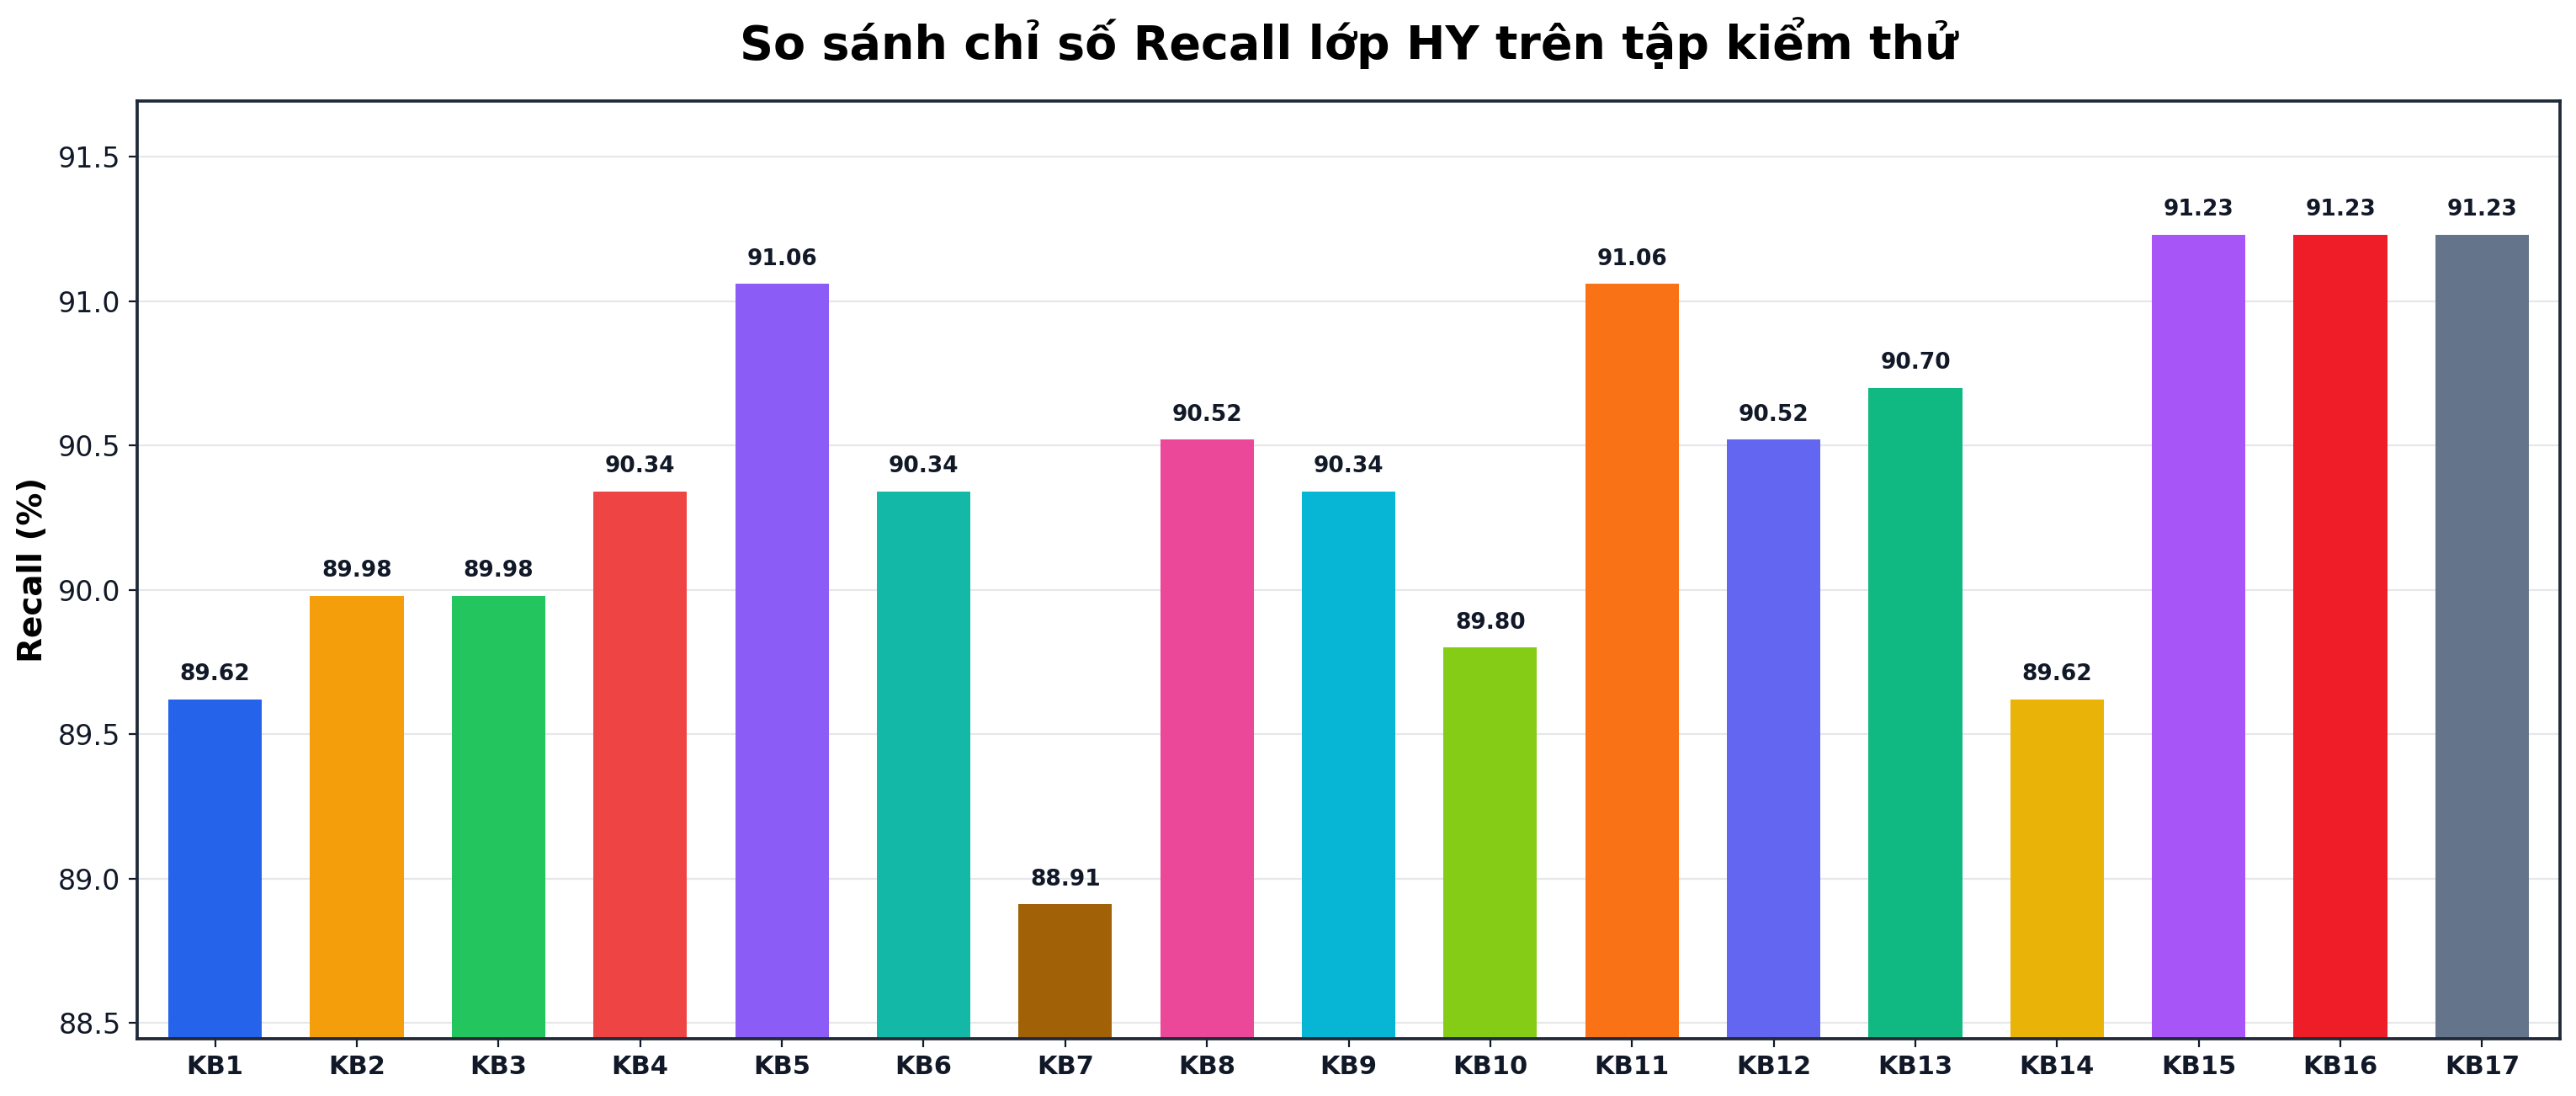
\includegraphics[width=\textwidth]{acc-loss/metric_recall_hy_test.png}
    \caption{Recall of the HY (High Yield) class}
    \label{fig:Recall_hy}
\end{subfigure}
\end{figure}

\begin{figure}[H]
\ContinuedFloat
\centering
\begin{subfigure}{\fairfigurewidth}
    \centering
    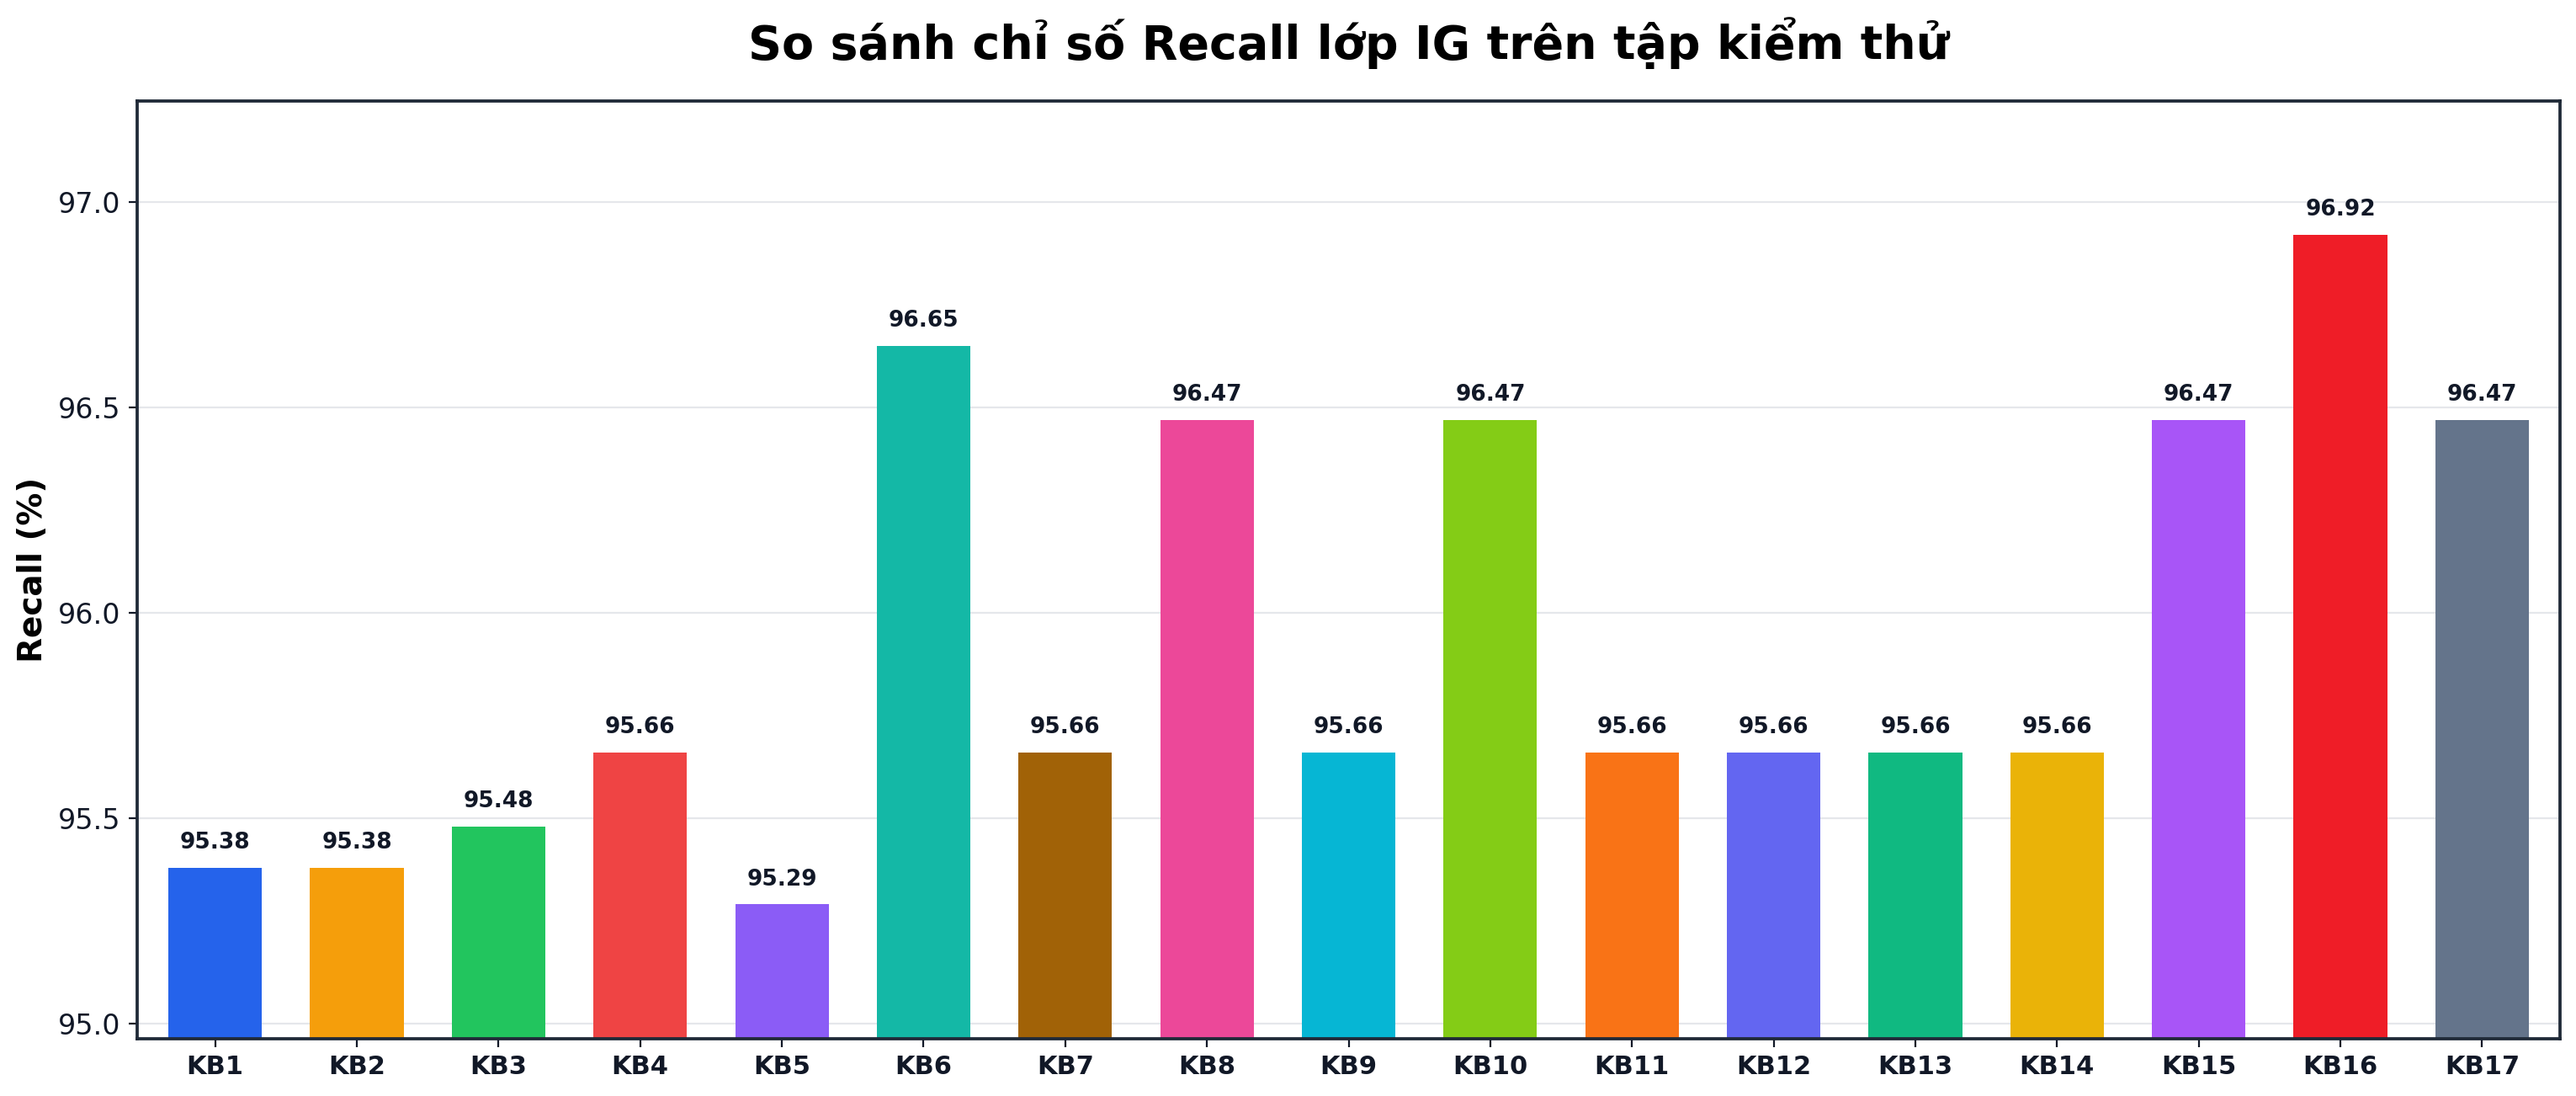
\includegraphics[width=\textwidth]{acc-loss/metric_recall_ig_test.png}
    \caption{Recall of the IG (Investment Grade) class}
    \label{fig:Recall_ig}
\end{subfigure}
\caption{Recall of the Distressed (a), HY (b), and IG (c) classes on the test set}
\label{fig:Recall_classes}
\end{figure}
Recall indicates the ability to identify all samples belonging to each credit-rating class.
The results show that Distressed is the most difficult class to identify and has large variation across models.
GraphSAGE achieves the highest Recall for Distressed at 62.71\%, indicating an advantage in detecting high-risk firms.
Fuzzy Ensemble scenarios provide relatively stable improvement but do not surpass GraphSAGE for this class.
The DMF group is not particularly prominent in covering the Distressed class.
For HY, model Recall is fairly stable, mainly within the 89\%--91\% range. DMF-LT, DMF-TG, and DMF-LTG achieve the highest HY Recall at 91.23\%. For IG, most models achieve high Recall, indicating strong recognition of firms with good credit quality.
DMF-TG achieves the highest IG Recall at 96.92\%.
Overall, GraphSAGE is more suitable when prioritizing Distressed-class detection, whereas DMF-TG is prominent for HY and IG.

\subsubsection{F1-score of the scenarios}
\begin{figure}[H]
\centering
\setupfairsubfigures
\begin{subfigure}{\fairfigurewidth}
    \centering
    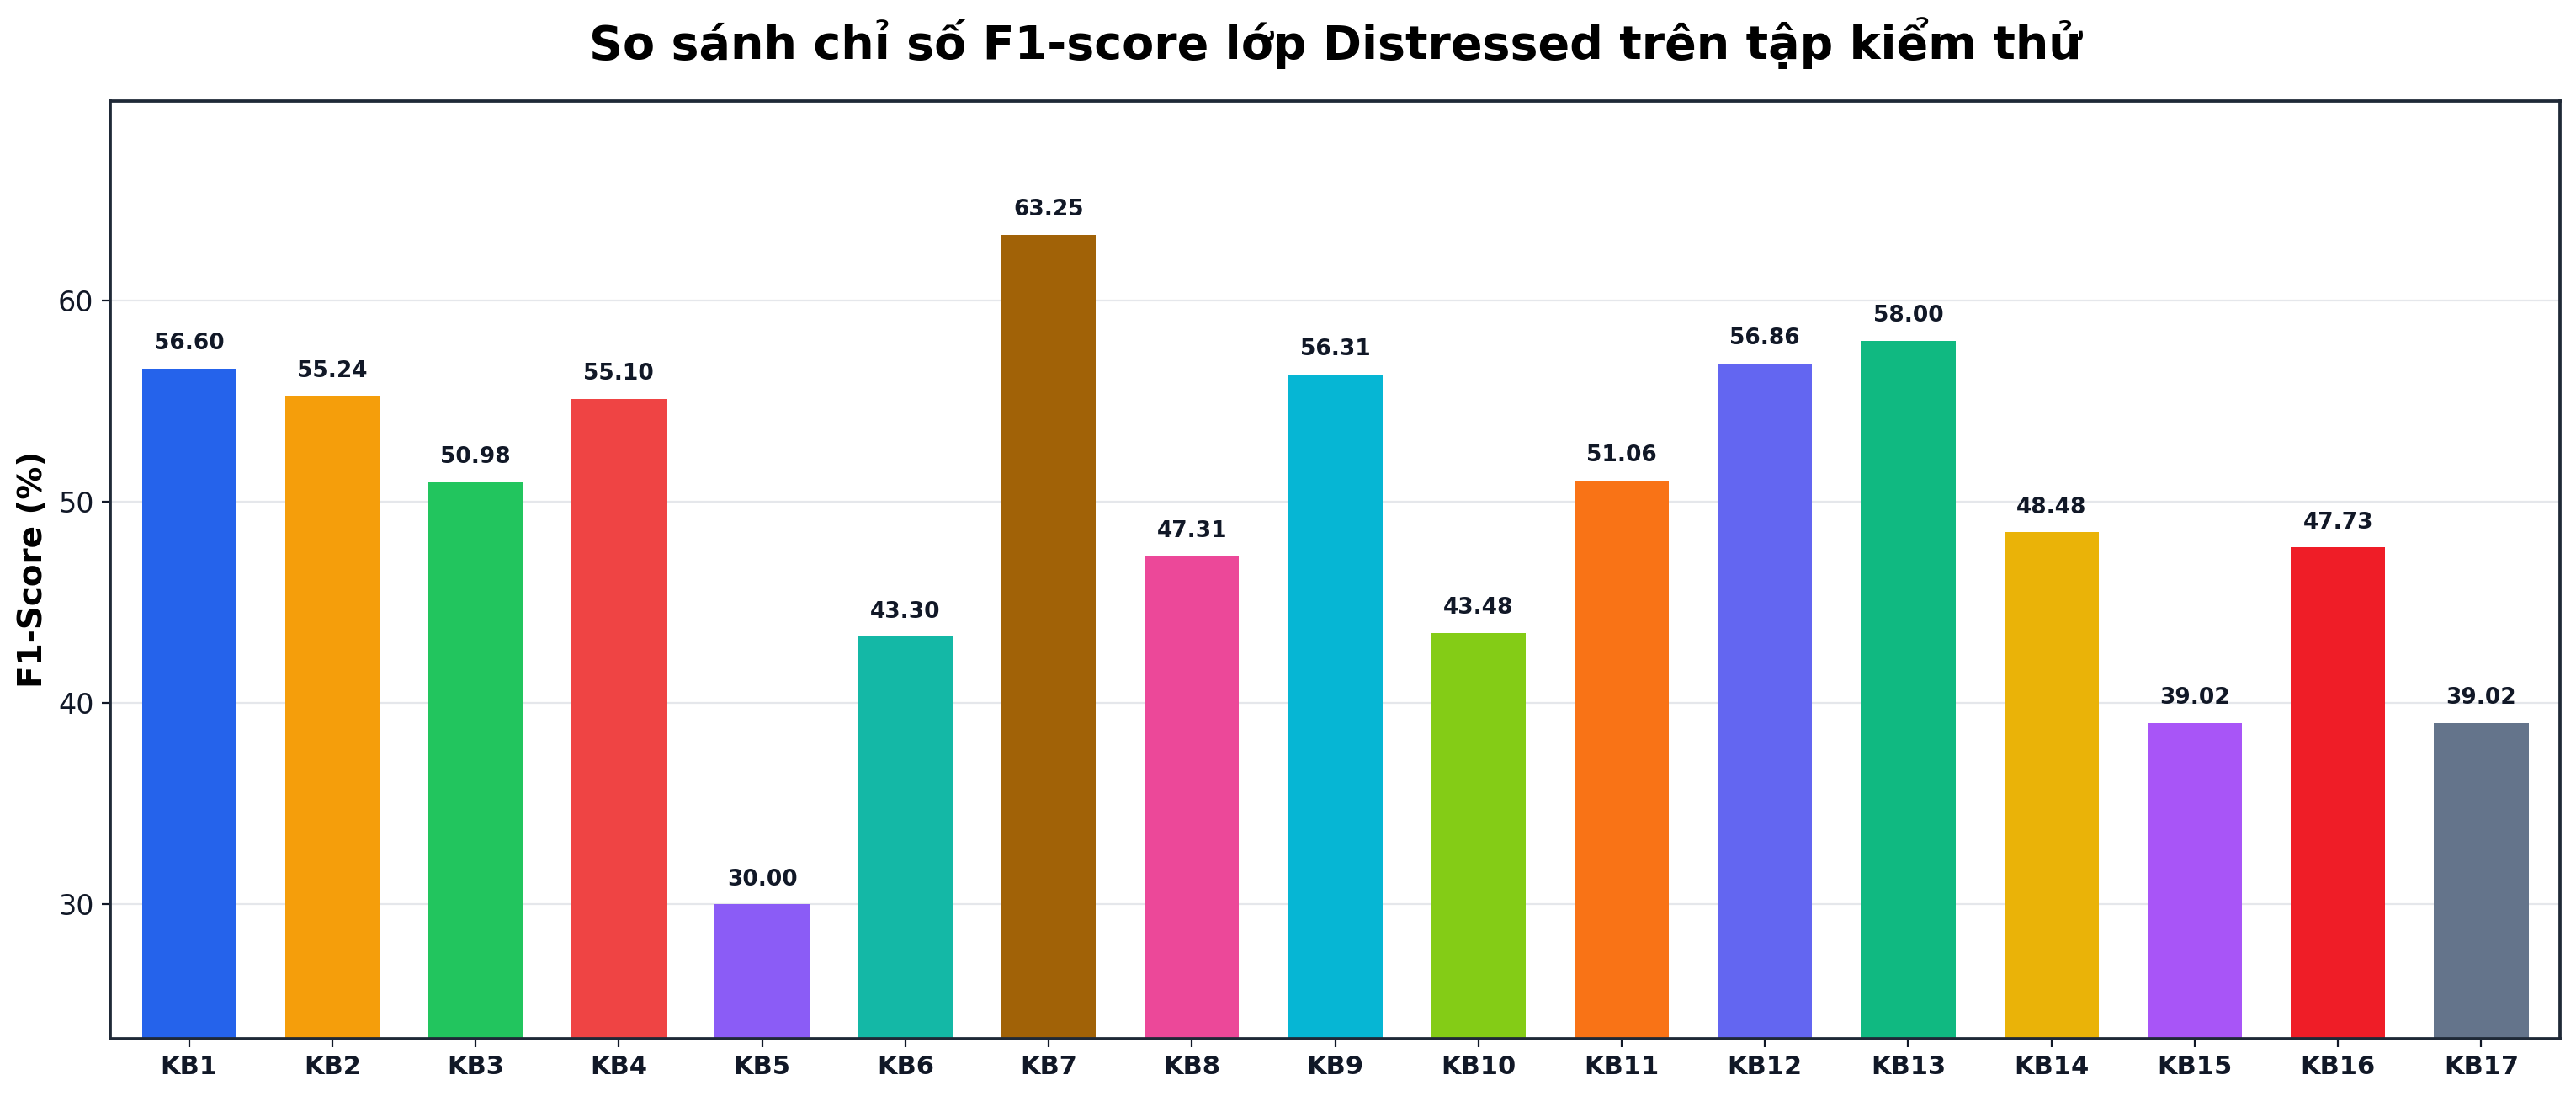
\includegraphics[width=\textwidth]{acc-loss/metric_f1_distressed_test.png}
    \caption{F1-score of the Distressed class}
    \label{fig:F1-Score_distressed}
\end{subfigure}
\end{figure}

\begin{figure}[H]
\ContinuedFloat
\centering
\begin{subfigure}{\fairfigurewidth}
    \centering
    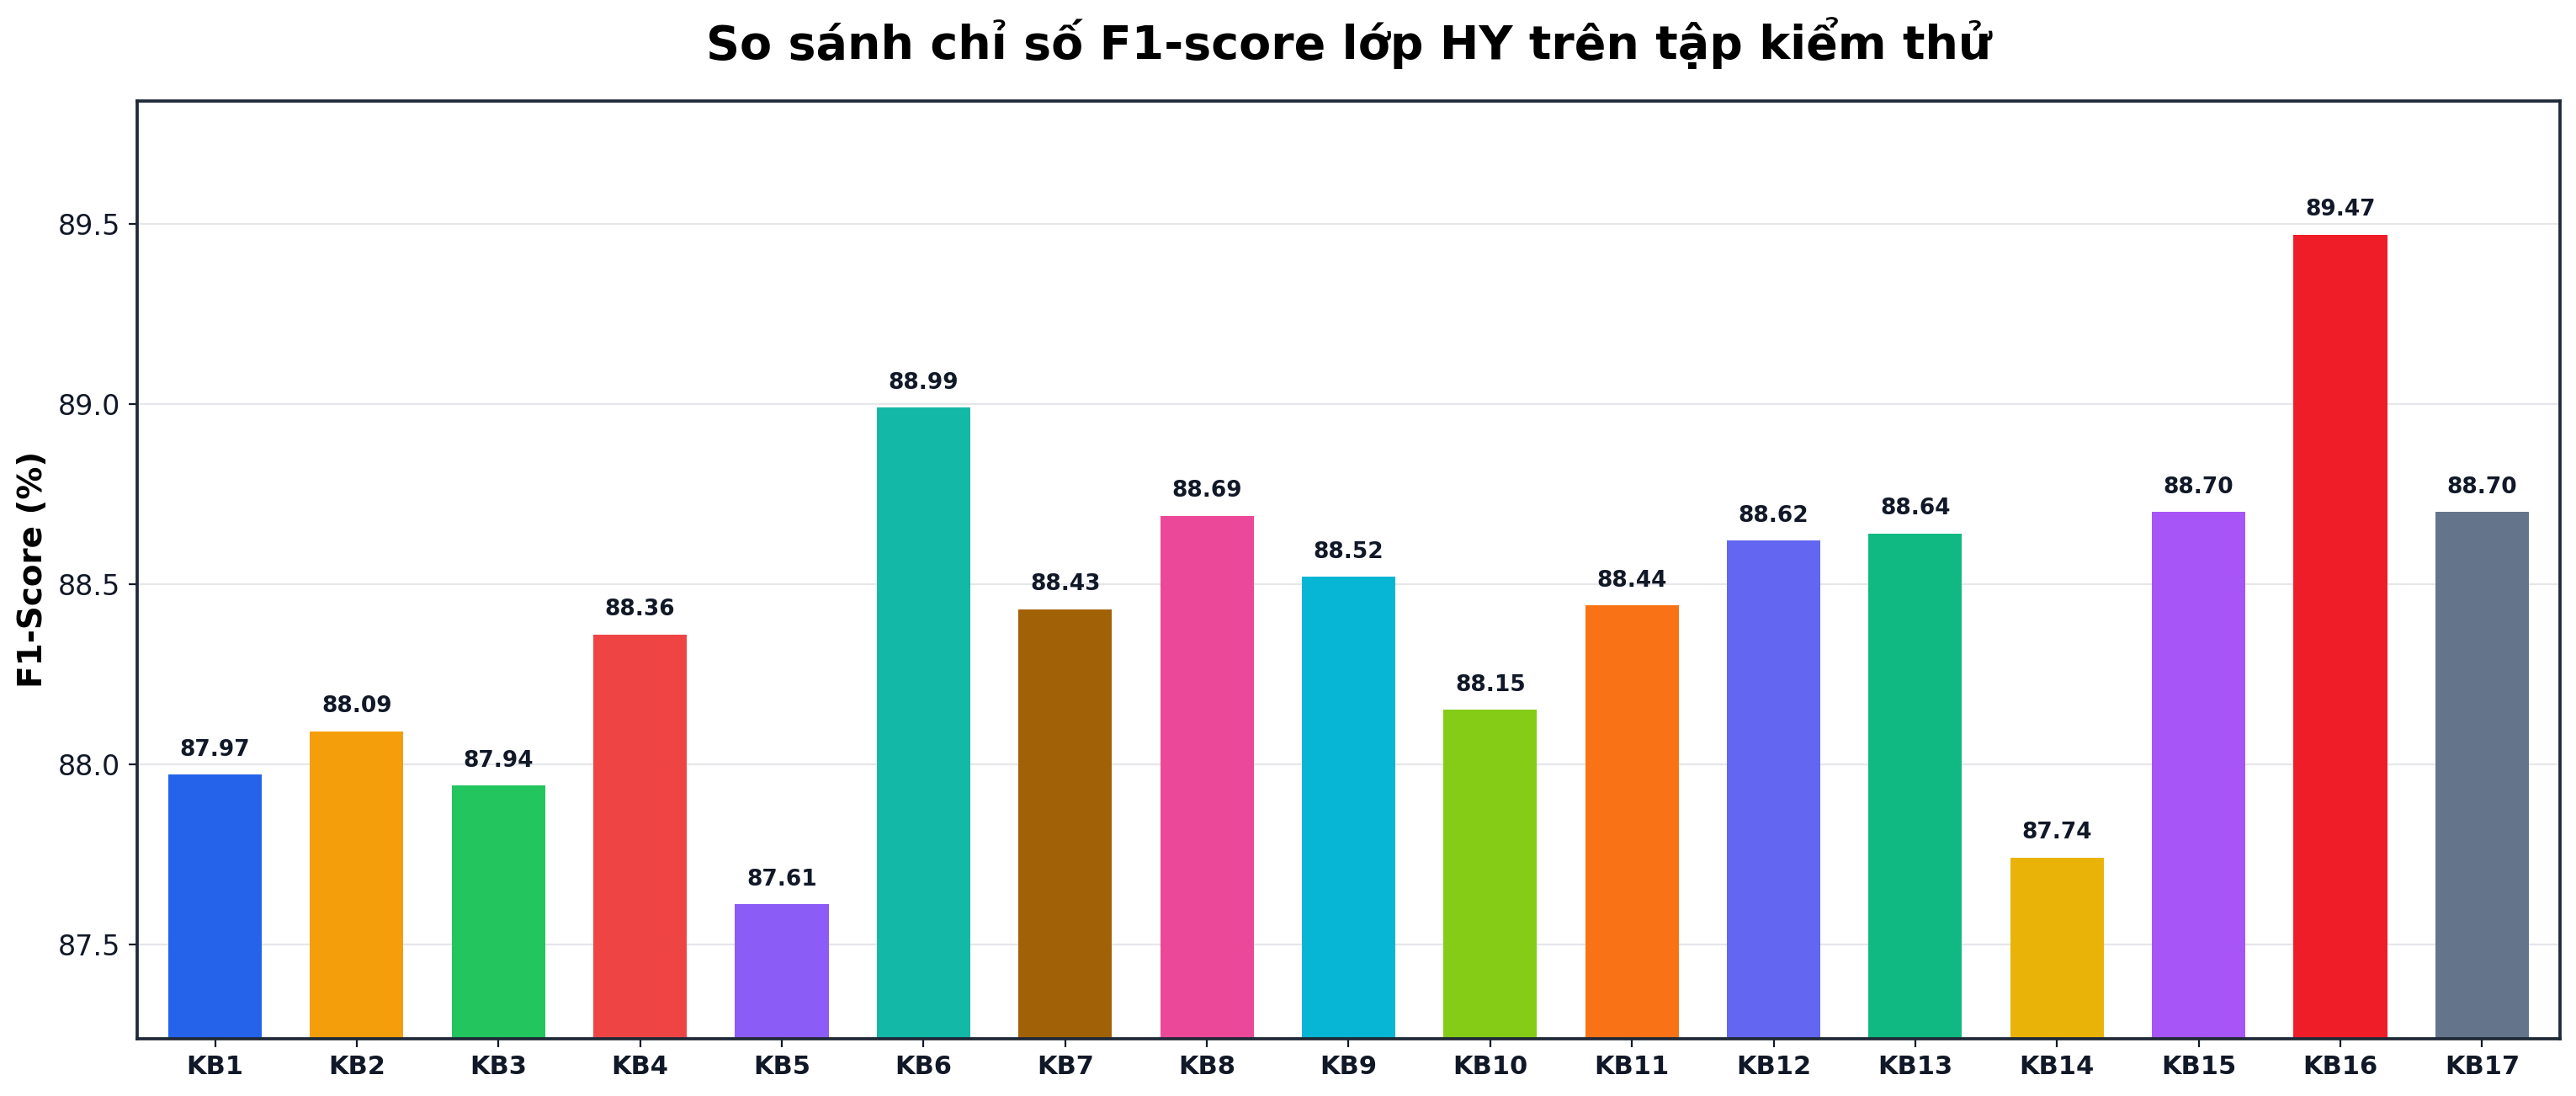
\includegraphics[width=\textwidth]{acc-loss/metric_f1_hy_test.png}
    \caption{F1-score of the HY (High Yield) class}
    \label{fig:F1-Score_hy}
\end{subfigure}
\end{figure}

\begin{figure}[H]
\ContinuedFloat
\centering
\begin{subfigure}{\fairfigurewidth}
    \centering
    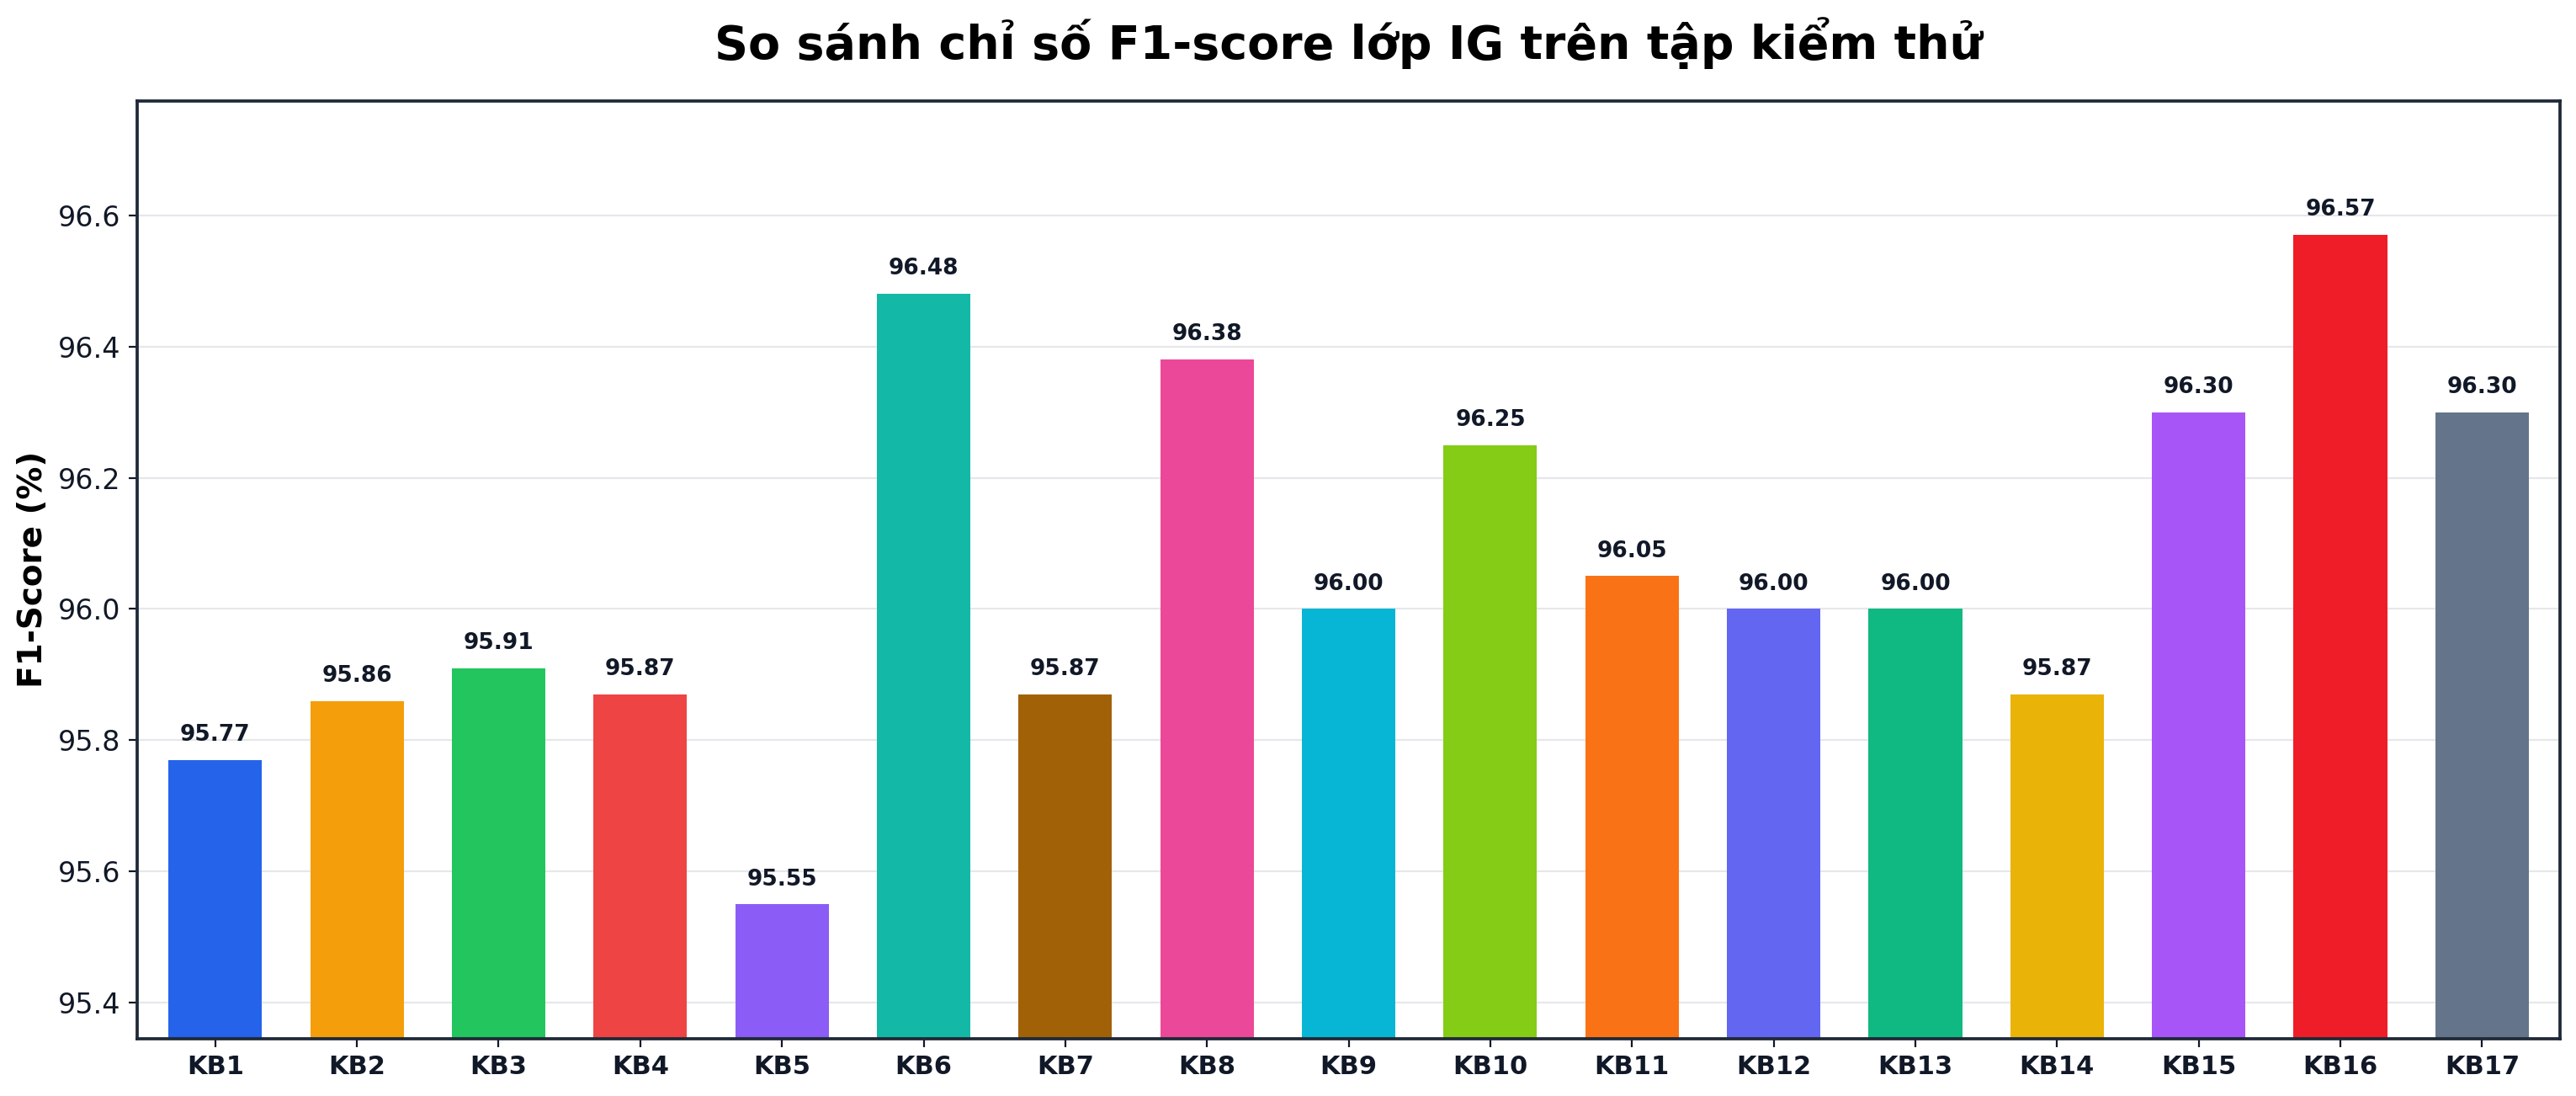
\includegraphics[width=\textwidth]{acc-loss/metric_f1_ig_test.png}
    \caption{F1-score of the IG (Investment Grade) class}
    \label{fig:F1-Score_ig}
\end{subfigure}
\caption{F1-score of the Distressed (a), HY (b), and IG (c) classes on the test set}
\label{fig:F1-Score_classes}
\end{figure}
F1-score reflects the balance between Precision and Recall for each credit-rating class. The results show that Distressed has the largest variation across models. GraphSAGE achieves the highest F1-score for Distressed at 63.25\%, indicating its advantage in identifying high-risk firms. LightGBM, XGBoost, and LSTM also achieve relatively good results, whereas PatchTST has the lowest F1-score for this class. In the Fuzzy Ensemble group, FR-TTLPXL obtains the best result for Distressed at 58.00\%. The DMF scenarios are not particularly prominent for Distressed, showing that detecting the high-risk group remains challenging. For HY, model F1-scores are fairly stable, mainly around 88\%--89\%. DMF-TG achieves the highest HY F1-score at 89.47\%.
For IG, most models achieve high F1-scores, with DMF-TG again leading at 96.57\%. Overall, GraphSAGE is more suitable when the Distressed class is prioritized, whereas DMF-TG is prominent for HY and IG.



\subsubsection{AUC-ROC of the scenarios}

\begin{figure}[H]
\centering
\setupfairsubfigures
\begin{subfigure}{\fairfigurewidth}
    \centering
    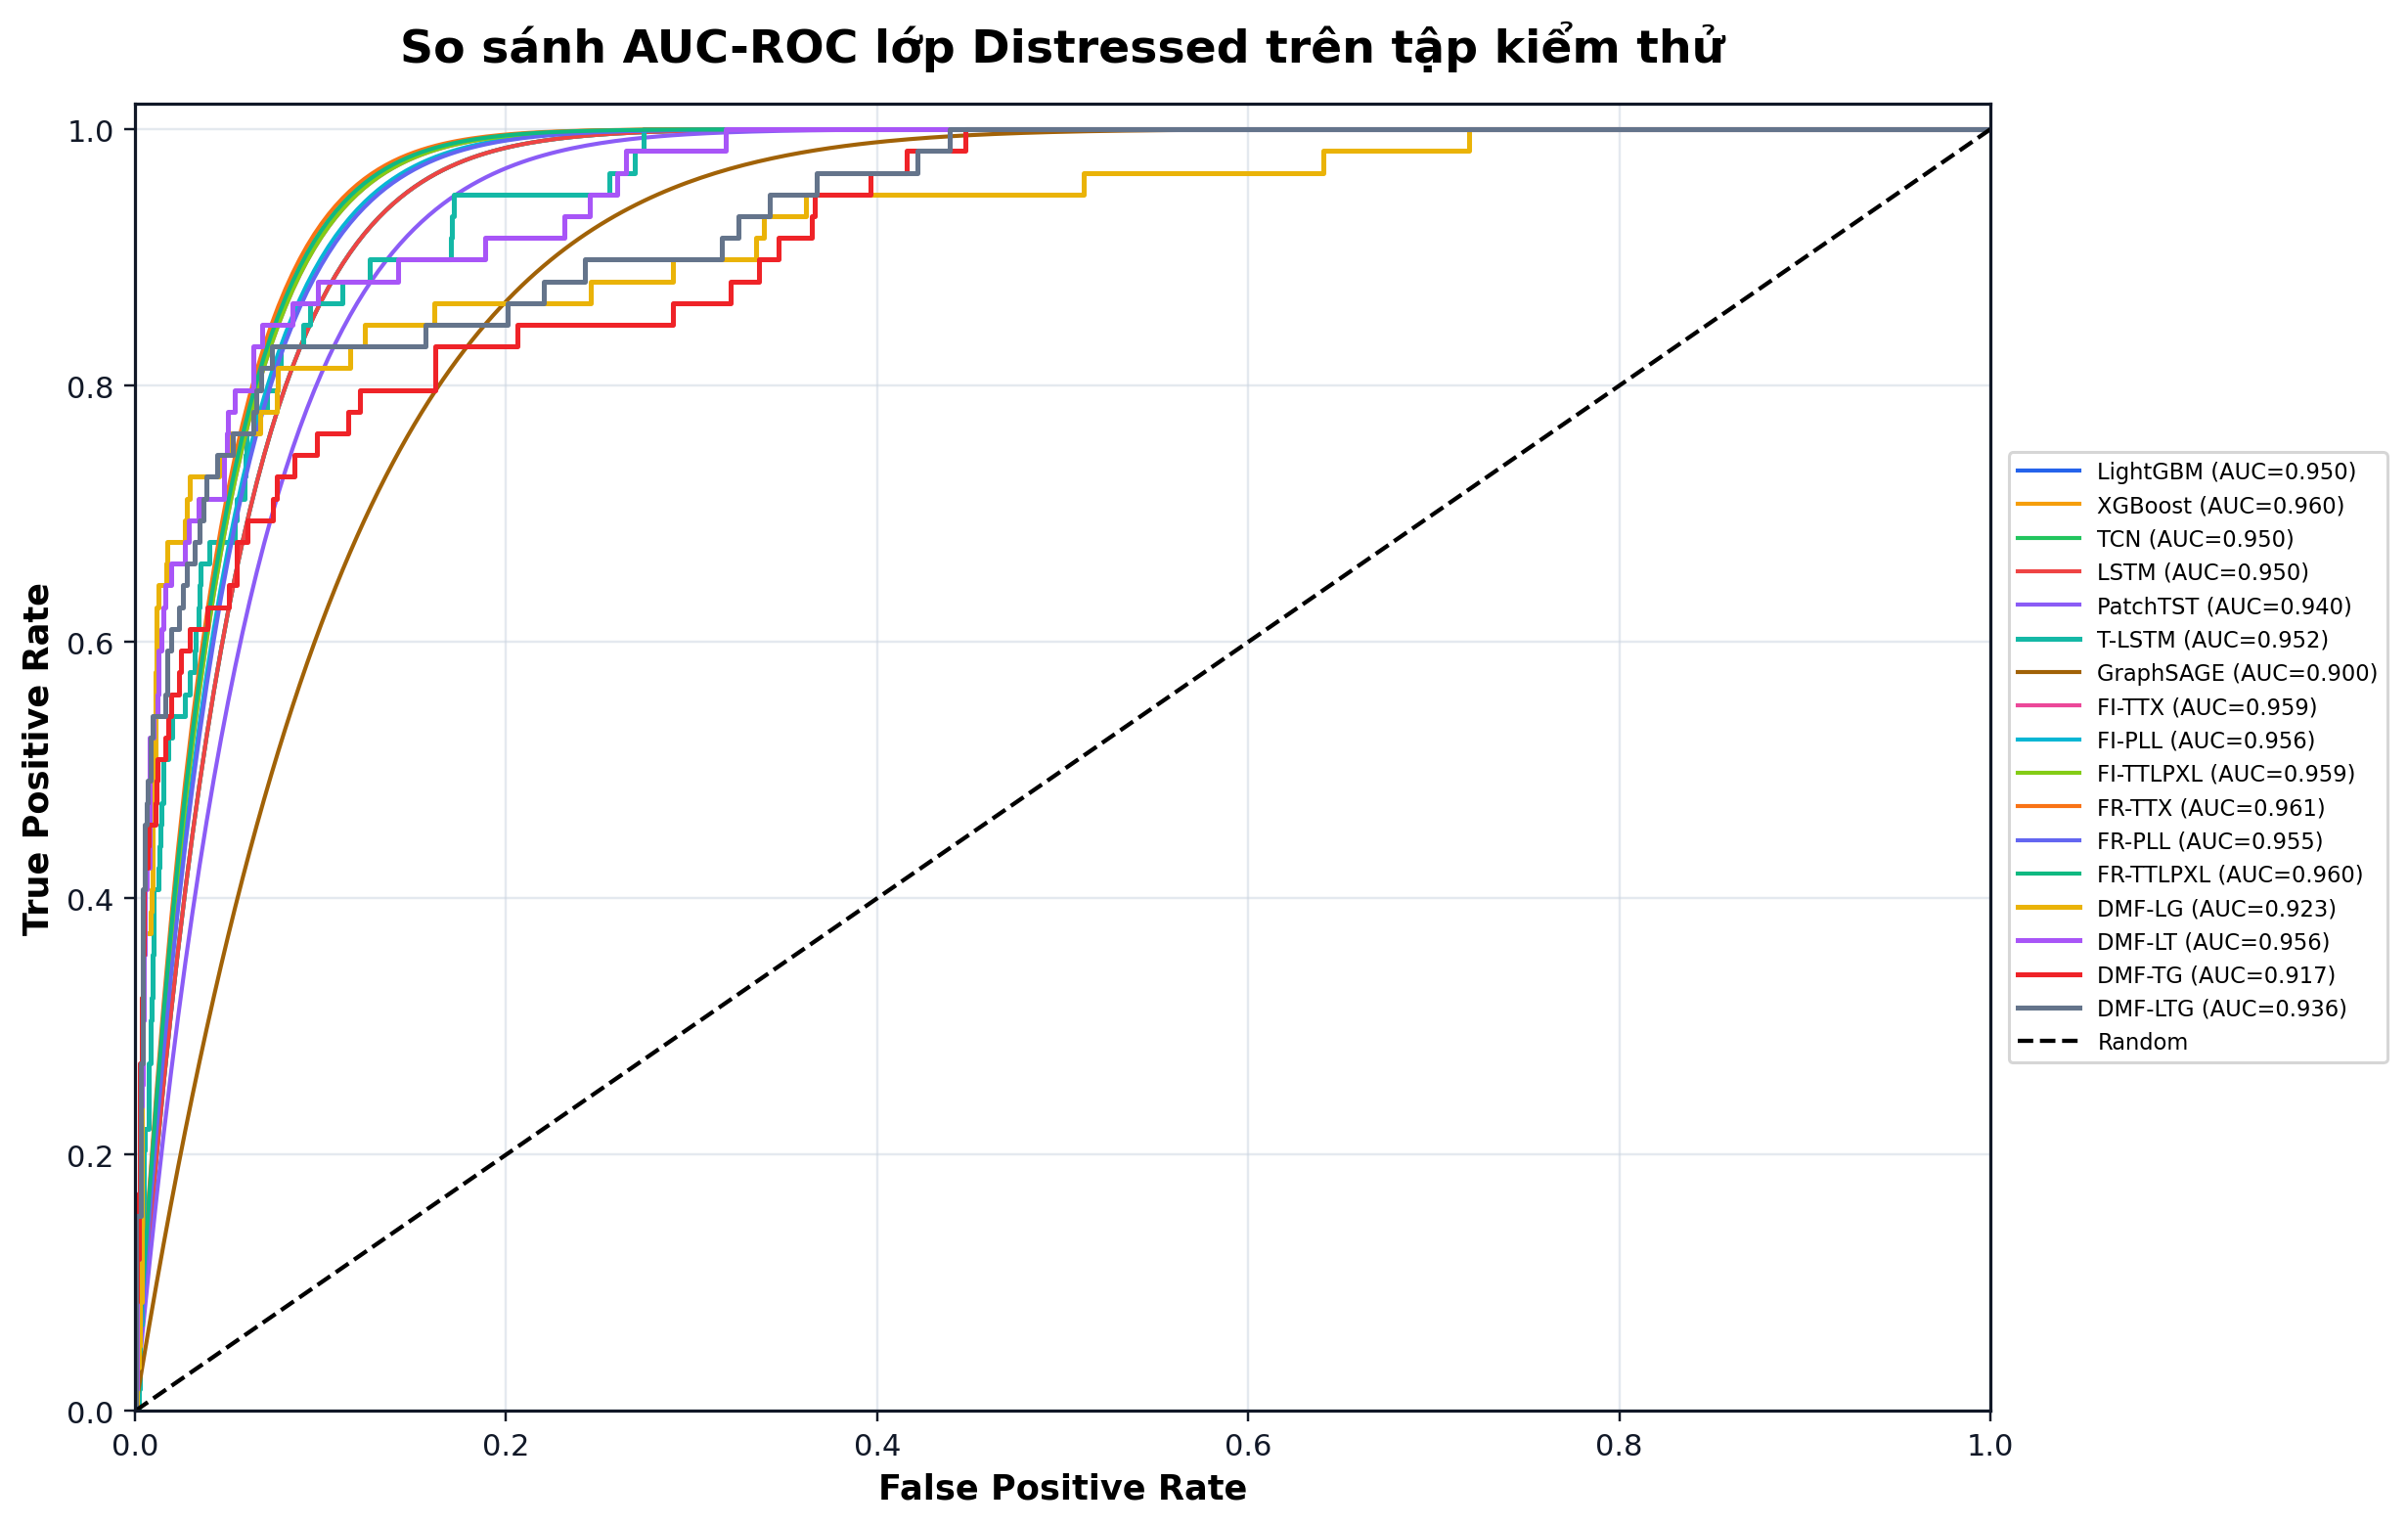
\includegraphics[width=\textwidth]{acc-loss/roc_distressed_17_models.png}
    \caption{ROC curves for the Distressed class}
    \label{fig:AUC-ROC_distressed}
\end{subfigure}
\end{figure}

\begin{figure}[H]
\ContinuedFloat
\centering
\begin{subfigure}{\fairfigurewidth}
    \centering
    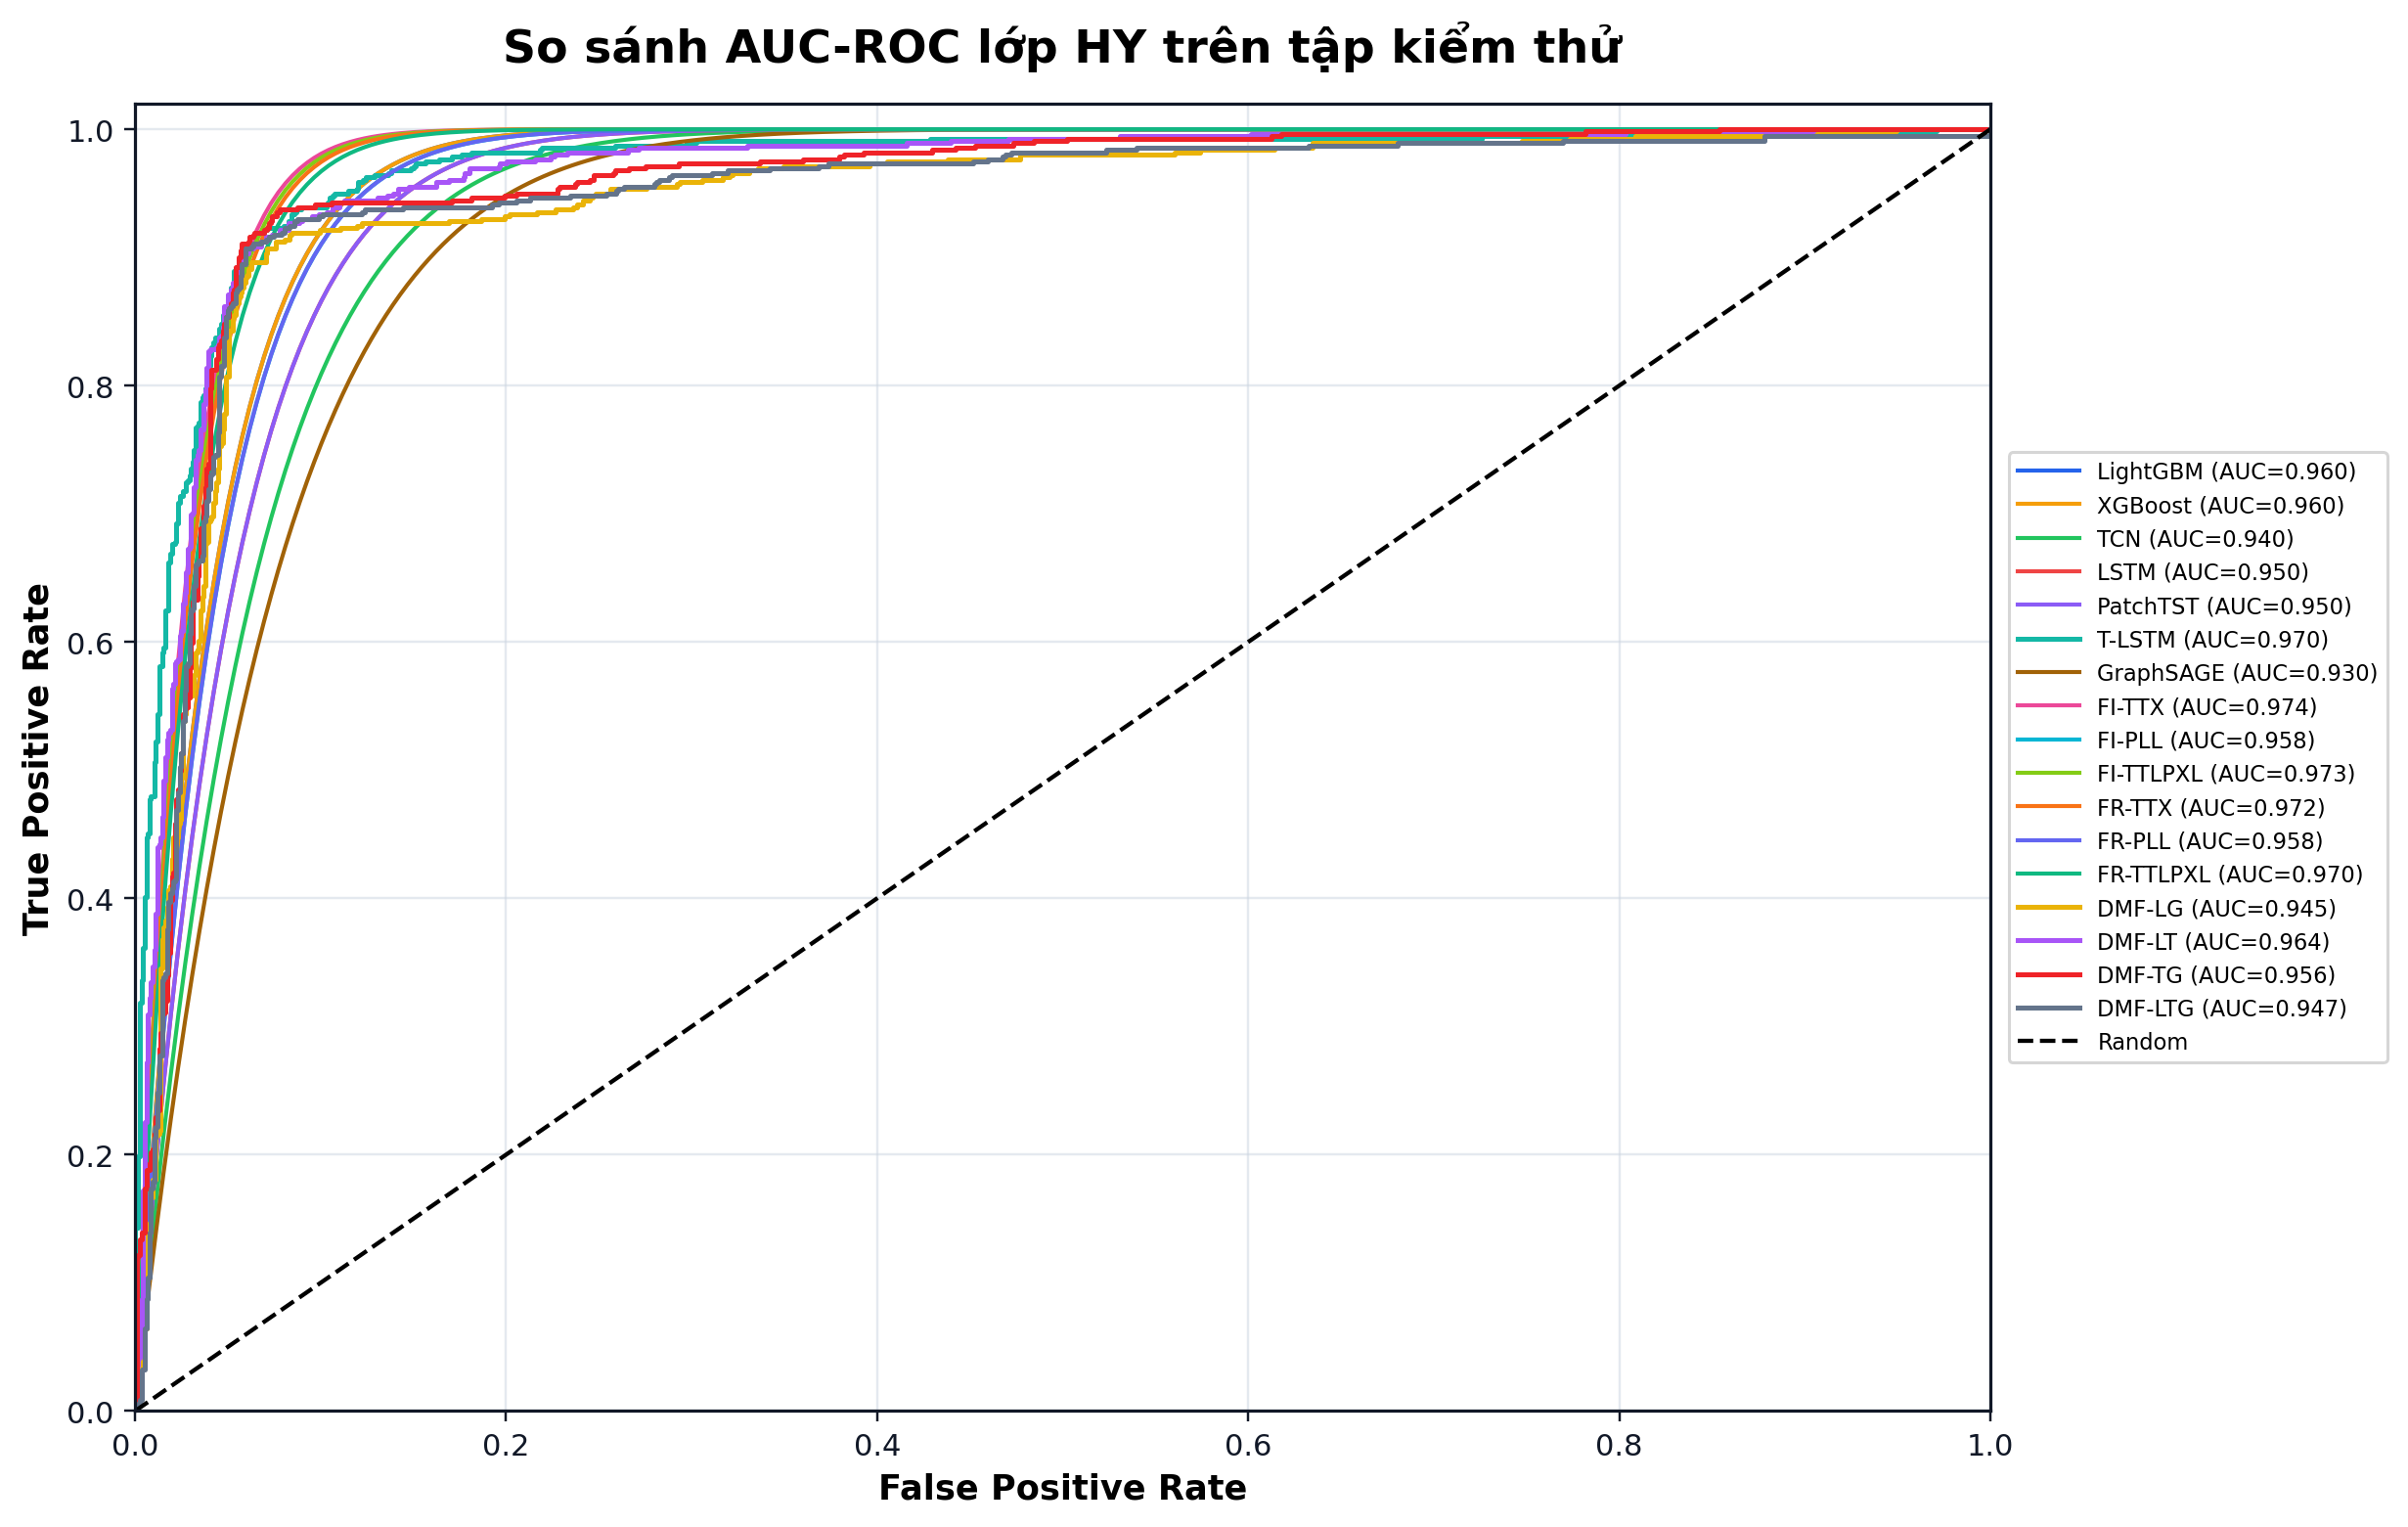
\includegraphics[width=\textwidth]{acc-loss/roc_hy_17_models.png}
    \caption{ROC curves for the HY (High Yield) class}
    \label{fig:AUC-ROC_hy}
\end{subfigure}
\end{figure}

\begin{figure}[H]
\ContinuedFloat
\centering
\begin{subfigure}{\fairfigurewidth}
    \centering
    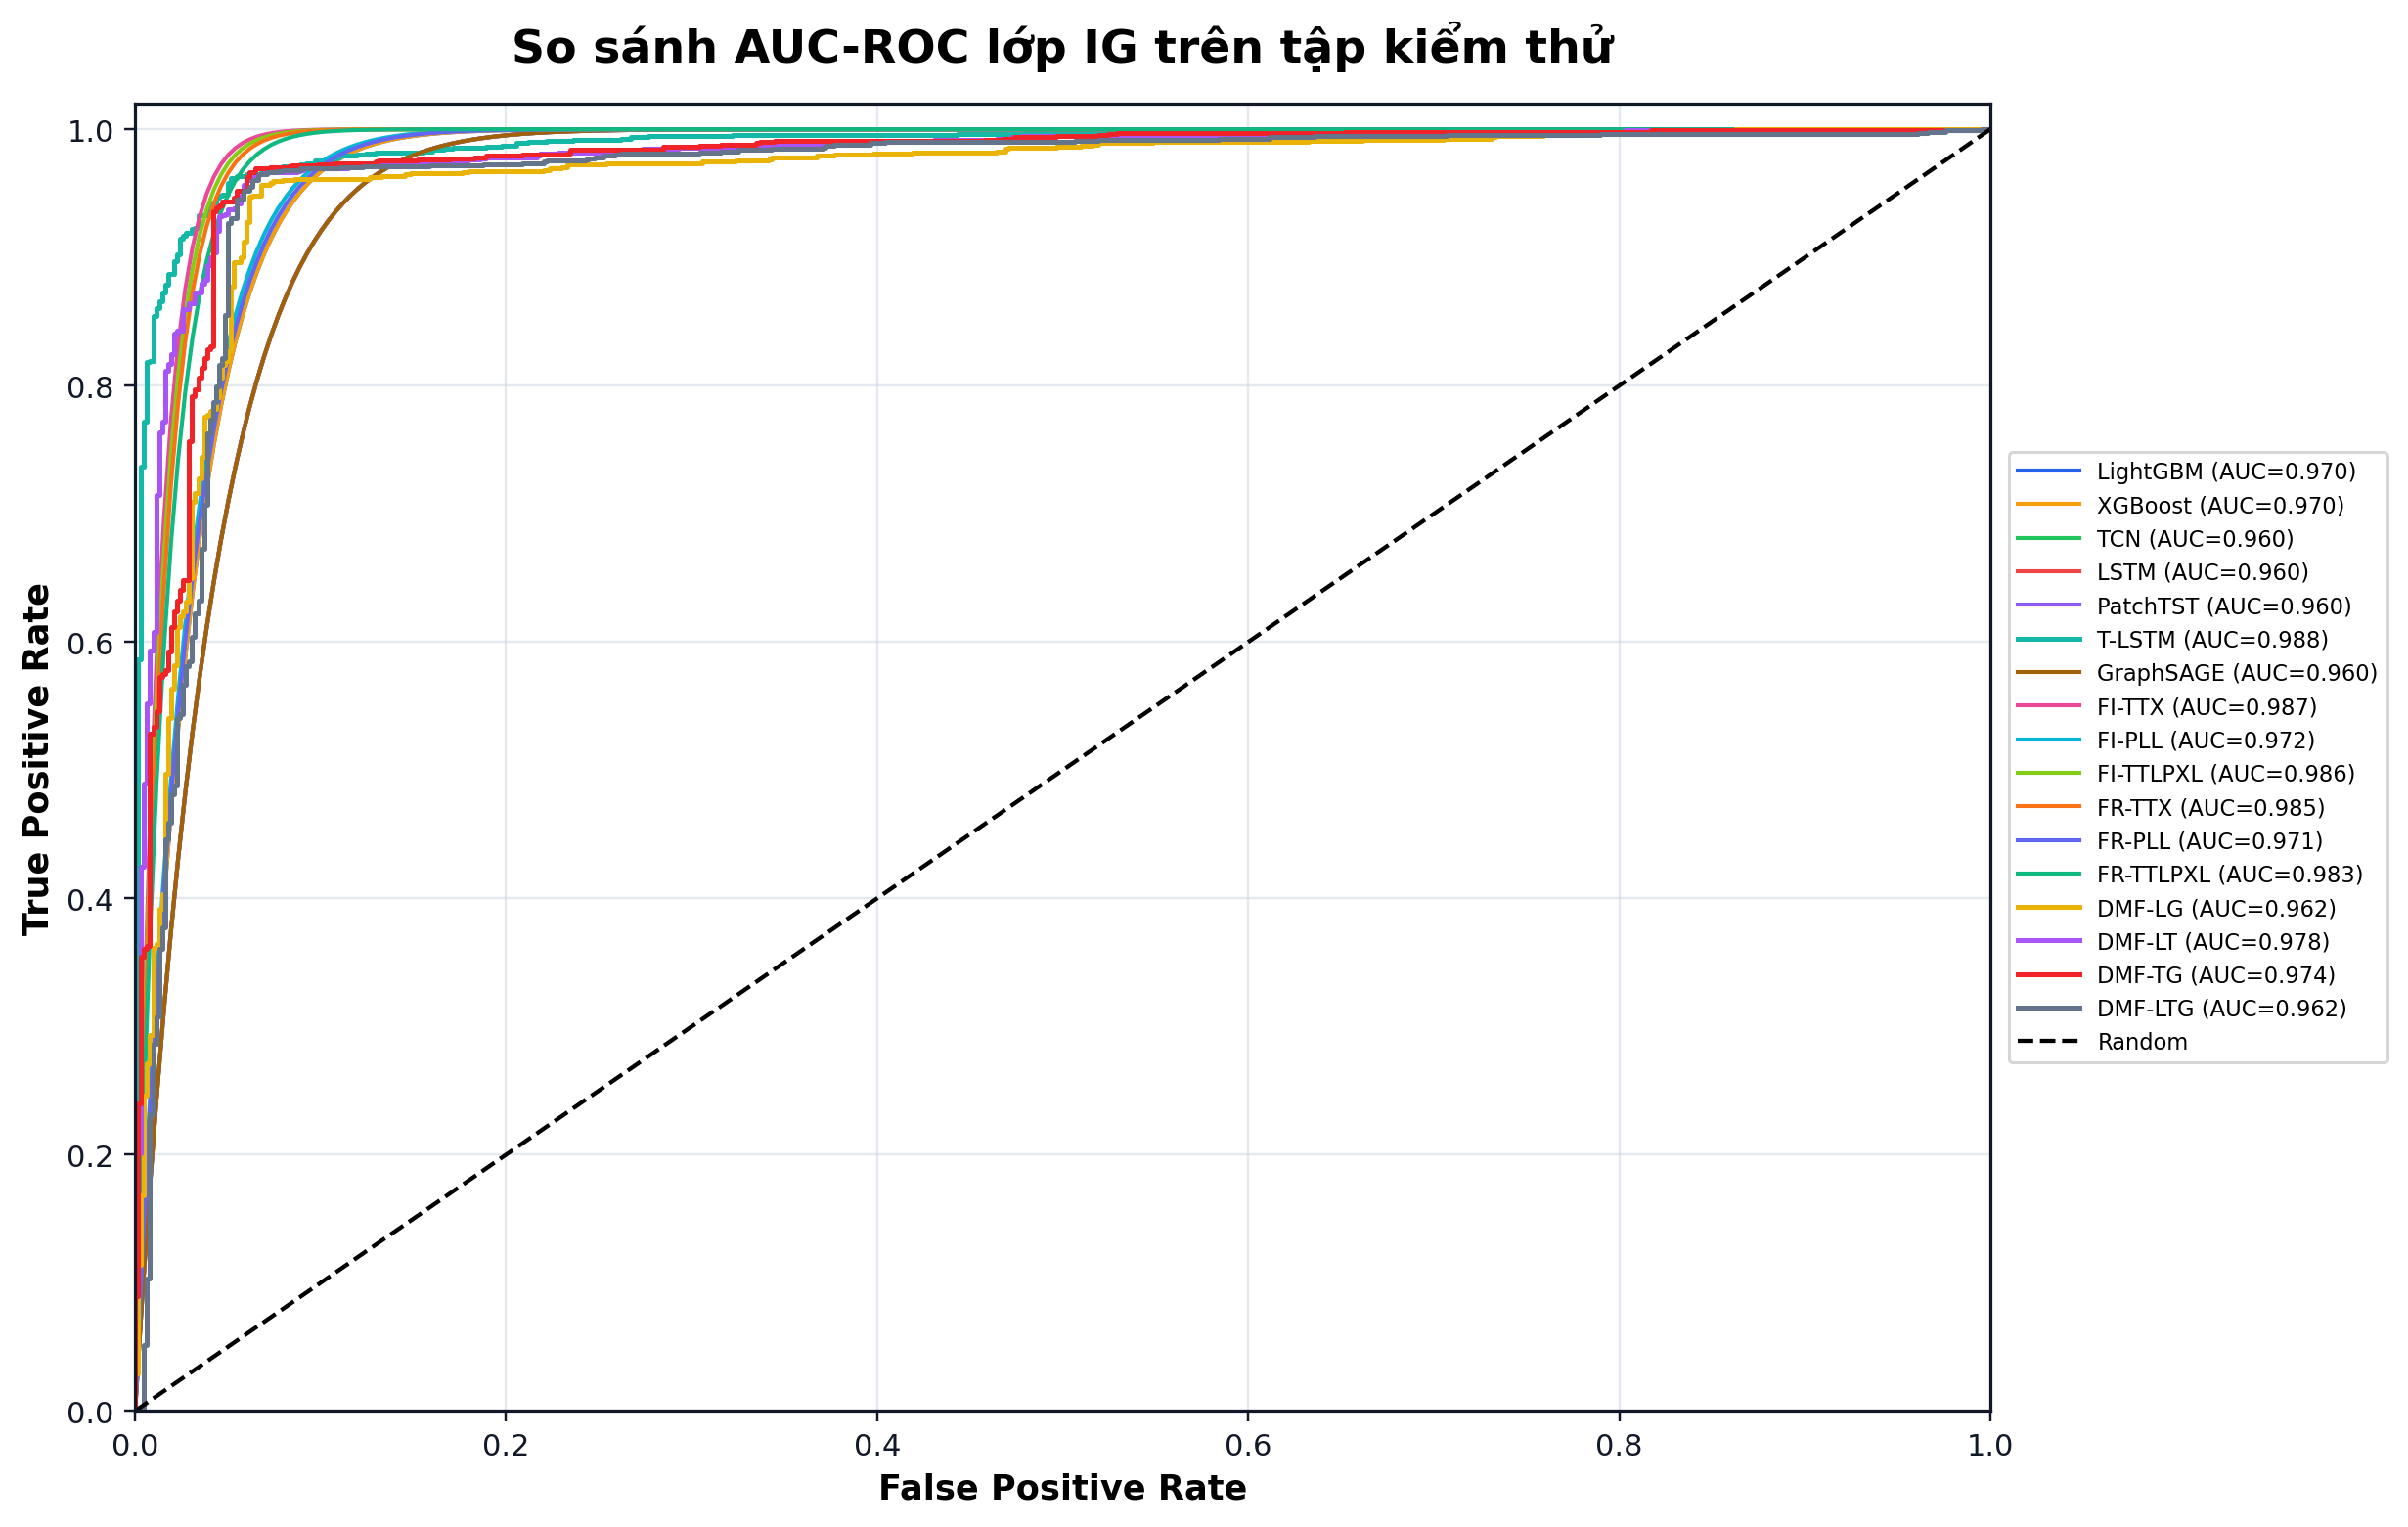
\includegraphics[width=\textwidth]{acc-loss/roc_ig_17_models.png}
    \caption{ROC curves for the IG (Investment Grade) class}
    \label{fig:AUC-ROC_ig}
\end{subfigure}
\caption{AUC-ROC of the Distressed (a), HY (b), and IG (c) classes on the test set}
\label{fig:AUC-ROC_classes}
\end{figure}

The three ROC charts show that most models have curves far from the random diagonal, demonstrating good discrimination between each rating class and the remaining classes. For Distressed, FR-TTX obtains the highest AUC at 96.1\%, followed by XGBoost and FR-TTLPXL, both at 96\%. For HY, FI-TTX achieves the best result with an AUC of 97.4\%, indicating the effectiveness of Fuzzy Ensemble in distinguishing the medium-risk group. For IG, T-LSTM achieves the highest AUC at 98.8\%, reflecting very strong recognition of firms with high credit quality. Overall, Fuzzy Ensemble scenarios such as FI-TTX, FR-TTX, and FI-TTLPXL achieve strong AUC values across several classes, whereas DMF has high overall Accuracy but is not the best model in class-specific AUC.

\subsubsection{Inference time}
\begin{figure}[H]
    \centering
    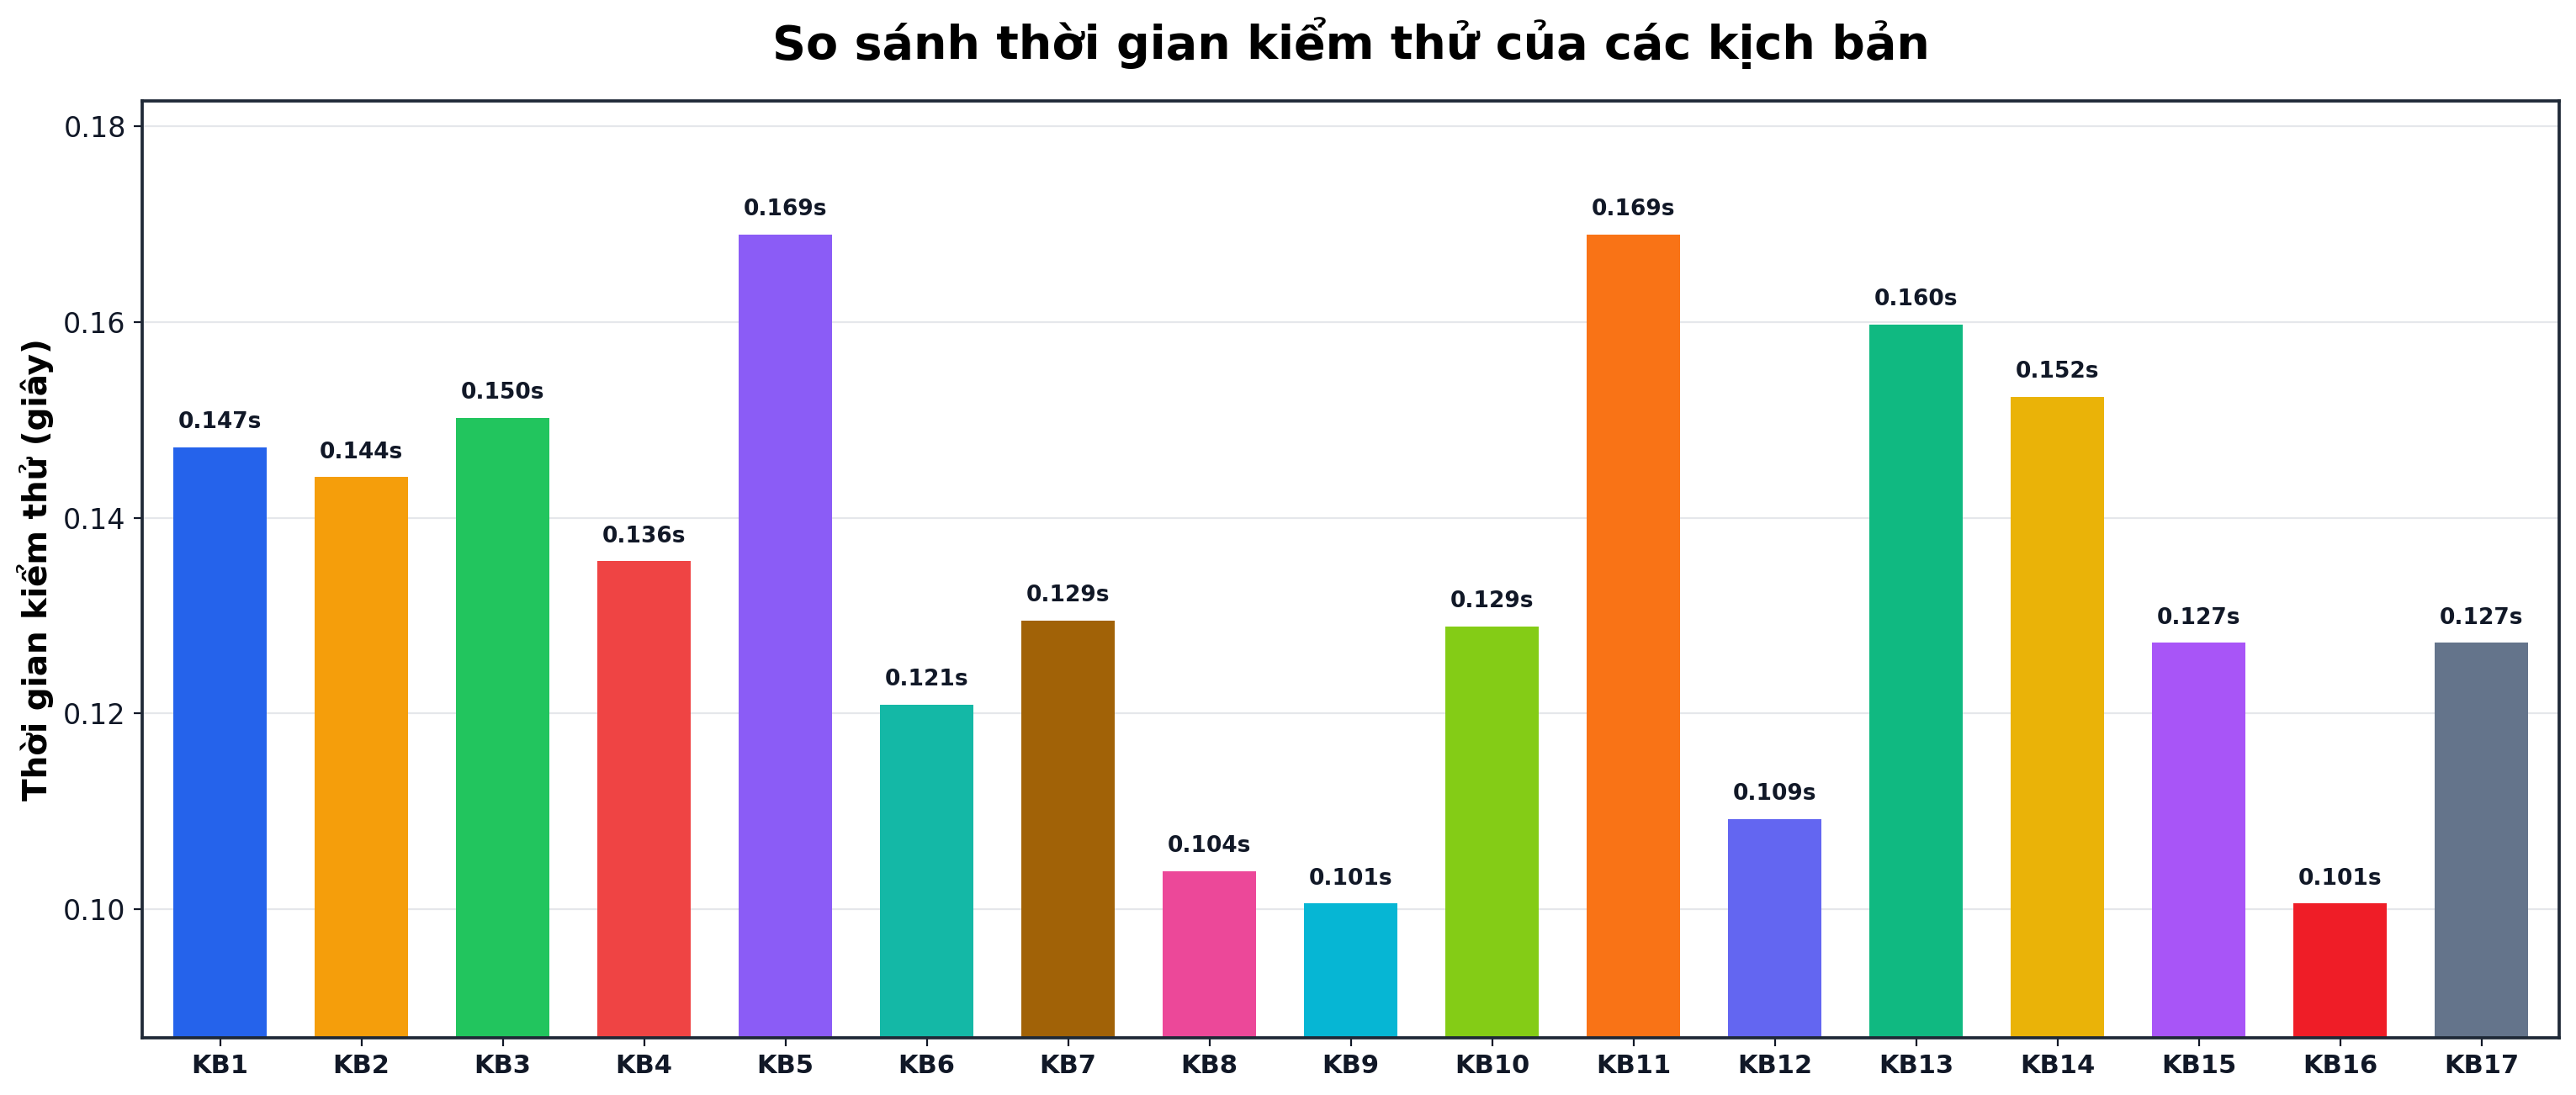
\includegraphics[width=\fairfigurewidth]{acc-loss/metric_inference_time_test_scenarios.png}
    \caption{Inference time of the scenarios}
\end{figure}
Test results show that the inference time of the 17 models and fusion scenarios is very low, ranging from 0.101 seconds to 0.169 seconds. This demonstrates that the models can predict quickly and are suitable for practical deployment requirements. Among individual models, T-LSTM achieves the lowest inference time at 0.121 seconds, whereas PatchTST has the highest time at 0.169 seconds. The remaining models, including GraphSAGE, LSTM, LightGBM, XGBoost, and TCN, have relatively stable inference times. For the Fuzzy Ensemble group, FI-PLL and FI-TTX provide fast inference, reaching 0.101 seconds and 0.104 seconds, respectively. Within the Dynamic Model Fusion group, DMF-TG achieves the lowest inference time at 0.101 seconds. 
\subsubsection{XAI explanation results}
\paragraph{GradientSHAP}
GradientSHAP is used to measure the contribution of each financial indicator to the model's predicted probability. This method is implemented directly on the trained model and does not use a surrogate model. Sequential financial features are reduced by taking the mean over the time window, after which GradientSHAP estimates the contribution of each variable through multiple samples between the instance to be explained and the background set.

\xairesultfigure{GradientSHAP results for Scenario 1}{gradientshap-scenario-1}{acc-loss/xai_shap_lightgbm.png}

Figure 4.10 presents the explanation results for the LightGBM model using GradientSHAP. The horizontal axis represents the mean absolute contribution value \(\mathrm{mean}\left(\left|\mathrm{GradientSHAP\ attribution}\right|\right)\), while the vertical axis lists the input financial indicators. Longer bars indicate that the corresponding feature has a larger influence on the model's predicted probability.
The results show that Pretax Profit Margin, Operating Profit Margin, Debt Equity Ratio, and Current Ratio are the most influential features. This indicates that the LightGBM model mainly relies on profitability, leverage, and liquidity to make credit-rating decisions. Indicators such as Ebit Margin, Operating Cashflow PS, and Net Profit Margin also contribute considerably, reflecting the role of profit and cash flow in assessing corporate financial health. Conversely, features such as Asset Turnover, Gross Profit Margin, and ROE have lower influence in this scenario.
This also provides a basis for analogous comparisons with the remaining scenarios to determine whether other models focus on the same important groups of financial indicators.


\xairesultfigure{GradientSHAP results for Scenario 2}{gradientshap-scenario-2}{acc-loss/xai_shap_xgboost.png}

\xairesultfigure{GradientSHAP results for Scenario 3}{gradientshap-scenario-3}{acc-loss/xai_shap_tcn.png}

\xairesultfigure{GradientSHAP results for Scenario 4}{gradientshap-scenario-4}{acc-loss/xai_shap_lstm.png}

\xairesultfigure{GradientSHAP results for Scenario 5}{gradientshap-scenario-5}{acc-loss/xai_shap_patchtst.png}

\xairesultfigure{GradientSHAP results for Scenario 6}{gradientshap-scenario-6}{acc-loss/xai_shap_tlstm.png}

\xairesultfigure{GradientSHAP results for Scenario 7}{gradientshap-scenario-7}{acc-loss/xai_shap_graphsage.png}

\xairesultfigure{GradientSHAP results for Scenario 8}{gradientshap-scenario-8}{acc-loss/xai_shap_fi_ttx.png}

\xairesultfigure{GradientSHAP results for Scenario 9}{gradientshap-scenario-9}{acc-loss/xai_shap_fi_pll.png}

\xairesultfigure{GradientSHAP results for Scenario 10}{gradientshap-scenario-10}{acc-loss/xai_shap_fi_ttlpxl.png}

\xairesultfigure{GradientSHAP results for Scenario 11}{gradientshap-scenario-11}{acc-loss/xai_shap_fr_ttx.png}

\xairesultfigure{GradientSHAP results for Scenario 12}{gradientshap-scenario-12}{acc-loss/xai_shap_fr_pll.png}

\xairesultfigure{GradientSHAP results for Scenario 13}{gradientshap-scenario-13}{acc-loss/xai_shap_fr_ttlpxl.png}

\xairesultfigure{GradientSHAP results for Scenario 14}{gradientshap-scenario-14}{acc-loss/xai_shap_dmf_lstm_graphsage.png}

\xairesultfigure{GradientSHAP results for Scenario 15}{gradientshap-scenario-15}{acc-loss/xai_shap_dmf_lstm_tlstm.png}

\xairesultfigure{GradientSHAP results for Scenario 16}{gradientshap-scenario-16}{acc-loss/xai_shap_dmf_tlstm_graphsage.png}

\xairesultfigure{GradientSHAP results for Scenario 17}{gradientshap-scenario-17}{acc-loss/xai_shap_dmf_lstm_tlstm_graphsage.png}

GradientSHAP records large contributions from features in the profitability, leverage, and liquidity groups. Pretax Profit Margin and Operating Profit Margin often appear among the highest-contribution features. Debt-to-Equity Ratio and Current Ratio are also used by many models when distinguishing risk groups. T-LSTM and GraphSAGE further distribute contributions to ROA, ROE, Asset Turnover, and cash-flow variables. For DMF/DCS, the prominent features include Pretax Profit Margin, Operating Profit Margin, Debt-to-Equity Ratio, and Current Ratio. These results are consistent with the commonly considered roles of profitability, leverage, and liquidity in credit analysis; they support interpretation of model behavior but do not establish causal relationships.

\paragraph{LIME}
LIME is used as a model-agnostic local explanation method. In this study, after a model produces a credit-rating prediction for a specific firm, LIME generates many perturbed samples around the original sample by slightly changing financial-feature values. These perturbed samples are then fed into the trained model to observe changes in predicted probabilities. 

\xairesultfigure{LIME results for Scenario 1}{lime-scenario-1}{acc-loss/xai_lime_lightgbm.png}

Figure 28 presents the local explanation results produced by LIME for a test sample in the LightGBM scenario. In the LIME chart, orange indicates features that support the class being explained, whereas blue indicates features that reduce the likelihood of that class. Bar length indicates each feature's influence on the local prediction.
For the IG class, features such as Pretax Profit Margin and ROE have positive effects, increasing the predicted probability of IG. Conversely, some variables such as Asset Turnover and Free Cashflow PS have opposite effects, although their influence is not large enough to change the final prediction. LIME is applied similarly to the remaining scenarios.



\xairesultfigure{LIME results for Scenario 2}{lime-scenario-2}{acc-loss/xai_lime_xgboost.png}

\xairesultfigure{LIME results for Scenario 3}{lime-scenario-3}{acc-loss/xai_lime_tcn.png}

\xairesultfigure{LIME results for Scenario 4}{lime-scenario-4}{acc-loss/xai_lime_lstm.png}

\xairesultfigure{LIME results for Scenario 5}{lime-scenario-5}{acc-loss/xai_lime_patchtst.png}

\xairesultfigure{LIME results for Scenario 6}{lime-scenario-6}{acc-loss/xai_lime_tlstm.png}

\xairesultfigure{LIME results for Scenario 7}{lime-scenario-7}{acc-loss/xai_lime_graphsage.png}

\xairesultfigure{LIME results for Scenario 8}{lime-scenario-8}{acc-loss/xai_lime_fi_ttx.png}

\xairesultfigure{LIME results for Scenario 9}{lime-scenario-9}{acc-loss/xai_lime_fi_pll.png}

\xairesultfigure{LIME results for Scenario 10}{lime-scenario-10}{acc-loss/xai_lime_fi_ttlpxl.png}

\xairesultfigure{LIME results for Scenario 11}{lime-scenario-11}{acc-loss/xai_lime_fr_ttx.png}

\xairesultfigure{LIME results for Scenario 12}{lime-scenario-12}{acc-loss/xai_lime_fr_pll.png}

\xairesultfigure{LIME results for Scenario 13}{lime-scenario-13}{acc-loss/xai_lime_fr_ttlpxl.png}

\xairesultfigure{LIME results for Scenario 14}{lime-scenario-14}{acc-loss/xai_lime_dmf_lstm_graphsage.png}

\xairesultfigure{LIME results for Scenario 15}{lime-scenario-15}{acc-loss/xai_lime_dmf_lstm_tlstm.png}

\xairesultfigure{LIME results for Scenario 16}{lime-scenario-16}{acc-loss/xai_lime_dmf_tlstm_graphsage.png}

\xairesultfigure{LIME results for Scenario 17}{lime-scenario-17}{acc-loss/xai_lime_dmf_lstm_tlstm_graphsage.png}
GradientSHAP and LIME provide two complementary levels of interpretation. GradientSHAP describes feature contributions across many observations, whereas LIME locally approximates model behavior around a specific prediction. The two methods help trace the financial indicators associated with predictions, thereby supporting system transparency. However, explanation results depend on the background sample, perturbation sampling strategy, and configuration of each method.
\subsection{Comparison and discussion}

\begingroup
\centering
\setlength{\tabcolsep}{4pt}
\renewcommand{\arraystretch}{1.05}
\begin{longtable}{c l c c c c}
\caption{Comparison of scenarios on the test dataset}
\label{tab:test_scenarios_comparison}\\
\hline
\textbf{Scenario} & \textbf{Scenario name} & \textbf{Accuracy (\%)} & \textbf{Precision (\%)} & \textbf{Recall (\%)} & \textbf{F1-score (\%)} \\
\hline
\endfirsthead
\caption[]{Comparison of scenarios on the test dataset (continued)}\\
\hline
\textbf{Scenario} & \textbf{Scenario name} & \textbf{Accuracy (\%)} & \textbf{Precision (\%)} & \textbf{Recall (\%)} & \textbf{F1-score (\%)} \\
\hline
\endhead
\hline
\multicolumn{6}{r}{\fairsmallfont Continued on the next page}\\
\endfoot
\hline
\endlastfoot
1  & LightGBM   & 91.99 & 91.88 & 91.99 & 91.90 \\
2  & XGBoost    & 92.05 & 91.94 & 92.05 & 91.95 \\
3  & TCN        & 91.93 & 91.76 & 91.93 & 91.78 \\
4  & LSTM       & 92.22 & 92.05 & 92.22 & 92.04 \\
5  & PatchTST   & 91.35 & 90.79 & 91.35 & 90.73 \\
6  & T-LSTM     & 92.51 & 92.10 & 92.51 & 92.23 \\
7  & GraphSAGE  & 92.34 & 92.35 & 92.34 & 92.34 \\
8  & FI-TTX     & 92.51 & 92.18 & 92.51 & 92.21 \\
9  & FI-PLL     & 92.34 & 92.20 & 92.34 & 92.22 \\
10 & FI-TTLPXL  & 92.16 & 91.75 & 92.16 & 91.82 \\
11 & FR-TTX     & 92.28 & 92.09 & 92.28 & 92.04 \\
12 & FR-PLL     & 92.40 & 92.26 & 92.40 & 92.27 \\
13 & FR-TTLPXL  & 92.46 & 92.33 & 92.46 & 92.31 \\
14 & DMF-LG     & 91.82	& 91.56	& 91.82 & 91.61 \\
15 & DMF-LT     & 92.40	& 92.02	& 92.40	& 91.87 \\
16 & DMF-TG     & \textbf{92.98} & \textbf{92.67} & \textbf{92.98} & \textbf{92.60} \\
17 & DMF-LTG    & 92.40	& 92.02	& 92.40	& 91.87 \\

\end{longtable}
\endgroup
Table~\ref{tab:test_scenarios_comparison} shows that all 17 scenarios achieve stable performance on the test set, with Accuracy ranging from 91.35\% to 92.98\%. Among individual models, T-LSTM achieves the best result, with Accuracy of 92.51\% and F1-score of 92.23\%, followed by GraphSAGE with an F1-score of 92.34\%. Fuzzy Ensemble scenarios generally maintain good performance, with FR-TTLPXL standing out at 92.46\% Accuracy and 92.31\% F1-score. In the Dynamic Model Fusion group, DMF-TG achieves the best result in the entire table, with Accuracy of 92.98\%, Precision of 92.67\%, Recall of 92.98\%, and F1-score of 92.60\%. Overall, DMF-TG is the most effective scenario, showing that dynamic fusion between T-LSTM and GraphSAGE improves corporate credit-rating classification performance.
\begingroup
\fontsize{9pt}{11pt}\selectfont
\renewcommand{\arraystretch}{1.08}
\setlength{\tabcolsep}{3pt}
\begin{longtable}{>{\raggedright\arraybackslash}p{3.0cm}
                  >{\raggedright\arraybackslash}p{5.0cm}
                  >{\raggedright\arraybackslash}p{3.2cm}
                  >{\centering\arraybackslash}p{1.8cm}}
\caption{Comparison between the proposed method and other methods}
\label{tab:comparison_proposed_method}\\
\hline
\textbf{Study} & \textbf{Dataset} & \textbf{Proposed method} & \textbf{Accuracy} \\
\hline
Liu and Kok \cite{liu_prediction_2025}
& Bureau van Dijk (BVD) data platform
& HTGNN
& 70.57\% \\

J. Darwish \cite{darwish_optimization_2025}
& National Information and Credit Evaluation, Inc. (NICE)
& Advanced feature selection
& 72.03\% \\

Morthens \cite{morthens_1989-_credit_2024}
& 318 firms for training and 112 firms unseen during training
& GRU; GRU-GCNGRU
& 75.25\%; 74.44\% \\

Mei Yang et al. \cite{yang_deep_2023}
& Compustat and Bloomberg
& HDNN
& 80.12\% \\

Sanjiv Das et al. \cite{das_credit_2023}
& Corporate Credit Rating and Synthetic Data
& GNN+Tabular
& 86.7\% \\

D. T. T. Thuy and T. L. Hai \cite{thuy_ung_2023}
& 300 Vietnamese firms over the 2017--2019 period
& XGBoost
& 87.73\% \\

Fang et al. \cite{fang_design_2025}
& Multimodal data from financial text, numerical indicators, and time series
& CNN-BiLSTM-AM
& 88\% \\

M. Kofune, K. Monden, and S. Yamanaka \cite{kofune_enhancing_2026}
& AstraManager database, provided by Quick Inc
& T-LSTM
& 89.96\% \\

\textbf{Proposed method}
& Corporate Credit Rating with Financial Ratios and Corporate Credit Rating
& DMF-TG
& 92.98\% \\
\hline
\end{longtable}
\endgroup

Table~\ref{tab:comparison_proposed_method} summarizes published results with Accuracy ranging from 70.57\% to 95\%. However, these studies use different datasets, class distributions, input features, and evaluation protocols; therefore, the values do not constitute a direct comparison. On the dataset used in the present study, DMF achieves an Accuracy of 92.98\%. The result indicates that combining T-LSTM and GraphSAGE is a promising direction for jointly exploiting temporal information and graph structure. Evaluating generalization requires additional datasets and unified experimental protocols.

\section{CONCLUSION}
This study developed a corporate credit-rating system based on machine-learning models, deep-learning models, graph models, and ensemble-learning methods. The input data were processed from financial indicators reflecting important aspects of firms, including liquidity, financial leverage, profitability, operating efficiency, and cash flow. On this basis, the system classifies firms into three credit-rating groups: Investment Grade (IG), High Yield (HY), and Distressed.

Methodologically, the study implemented several individual models, including LightGBM, XGBoost, LSTM, TCN, PatchTST, Transformer-LSTM, and GraphSAGE. In addition, it constructed model-fusion scenarios along two main directions. The first direction is Fuzzy Ensemble, including the Fuzzy Choquet Integral and Gompertz Fuzzy Ranking, to exploit the strengths of multiple component models. The second direction is Dynamic Model Fusion combined with Dynamic Classifier Selection, which allows the system to select the appropriate model for each data sample instead of using a fixed fusion rule. The models and scenarios were evaluated using Accuracy, Precision, Recall, F1-score, AUC-ROC, confusion matrix, training time, and inference time. Experimental results show that the models and fusion scenarios achieve relatively stable classification performance on the test set. Among them, the DMF-TG scenario, which combines Transformer-LSTM and GraphSAGE, obtains the best results, with Accuracy of 92.98\%, Precision of 92.67\%, Recall of 92.98\%, and F1-score of 92.60\%. This result indicates that dynamic fusion between a time-series model and a graph model can better exploit complementary information across architectures and thereby improve classification performance in corporate credit rating.

The main contribution of this study is the construction of a corporate credit-rating evaluation pipeline capable of combining multiple model types, including tabular machine-learning models, time-series deep-learning models, and graph models. In addition, the study extends ensemble-learning approaches through Fuzzy Ensemble and Dynamic Model Fusion scenarios, making the system more flexible in decision-making. Beyond predictive performance, the study integrates Explainable AI methods such as GradientSHAP and LIME to explain the influence of financial indicators on rating outcomes, thereby increasing transparency and helping users better understand the basis of model decisions.

Nevertheless, the study still has several limitations. The input data are mainly based on quantitative financial indicators and do not fully exploit nonfinancial data sources such as news, annual reports, industry data, or macroeconomic variables. The ability to identify the Distressed class remains limited because high-risk samples are fewer and the boundary between Distressed and HY is not fully clear. In addition, some deep-learning models such as T-LSTM, TCN, and PatchTST have higher training costs than tabular machine-learning models. Although XAI methods improve transparency, their explanation results mainly reflect model behavior and cannot be treated as absolute causal evidence in financial analysis.

In future work, the input data can be expanded by incorporating nonfinancial sources such as corporate news, annual reports, industry data, supply-chain information, and macroeconomic indicators. The dataset should also be updated to more recent periods to better reflect current economic conditions and market fluctuations. In addition, Distressed-class recognition should be improved through imbalance-handling techniques, class-weight adjustment, or more suitable loss functions. Further graph-model development can also incorporate inter-firm relationships such as industry affiliation, ownership, transactions, borrowing relationships, or supply chains. Finally, optimizing training time, inference time, and the application system will improve the practical deployability of the model for supporting corporate credit-risk assessment.

\bibliographystyle{IEEEtran}
\bibliography{thesis}

\end{document}
